\chapter{纤维化与 Yoneda 引理}\label{ch:fibrations-yoneda}


在本章中，我们的目标是描述由一个\trInfinityCategory{} $B$ 的\trElement{}
$b\colon 1\to B$ 所表示的反变\trFunctor{}的∞-范畴式编码；非形式地说，这一%
\trFunctor{}把 $B$ 的\trElement{} $x$ 送到定义 3.4.9 的\trMappingSpace{}
$\mathrm{Hom}_{B}(x,b)$。
由命题 3.4.10，这类\trRepresentable{}函子取值于\trDiscrete{}\trInfinityCategory，
后者在 $(\infty,1)$-\trCategory{}的诸\trInfinityCosmos{}中对应于「空间」或%
「\trInfinityGroupoid{}」。

与通常 1-\trCategory{}论的情形相比，在∞-范畴理论中，要把诸\trRepresentable{}%
函子显式地描述为诸∞-范畴之间的\trFunctor{}，是件颇有挑战性的事情。困难出现在
确立这一映射的∞-函子性上：它必须逐维地、以\trHomotopy{}相干的方式编码 $B$ 中
诸箭头的函子性作用，而这些数据即便在这个基本特例中也已繁复到难以轻易列举。
事实证明，较容易描述的是「\trElement{}范畴」的∞-范畴式类比——该范畴与映射
$x\mapsto\mathrm{Hom}_{B}(x,b)$ 相关联，并带有与之相关联的、到 $B$ 的一个投影。
事实上，我们对这个∞-范畴已然相当熟悉：它就是「右表示的」%
\trCommaInfinityCategory{} $\mathrm{Hom}_{B}(B,b)$，配上其定义域投影%
\trFunctor{} $p_{0}\colon\mathrm{Hom}_{B}(B,b)\twoheadrightarrow B$；后者在
$x\colon 1\to B$ 之上的\trFiber{}恰好复原出\trMappingSpace{}
$\mathrm{Hom}_{B}(x,b)$。

尚待说明的，是 $p_{0}\colon\mathrm{Hom}_{B}(B,b)\twoheadrightarrow B$ 在何种
意义上表达了 $B$ 中诸箭头在其诸\trFiber{}上的反变函子性作用。这一\trFunctor{}%
享有一条特殊性质：它使我们得以把取值于 $B$ 的\trNaturalTransformation{}以一种
本质唯一的方式提升为取值于 $\mathrm{Hom}_{B}(B,b)$、且余定义域已指定的%
\trNaturalTransformation。这种\trLifting{}的一个特例，定义出与%
\trHomotopyCategory{} $\mathrm{h}B$ 中一支箭头 $f\colon x\to y$ 相关联的%
\trPreComposition\trFunctor{} $f^{*}$：
\begin{center}
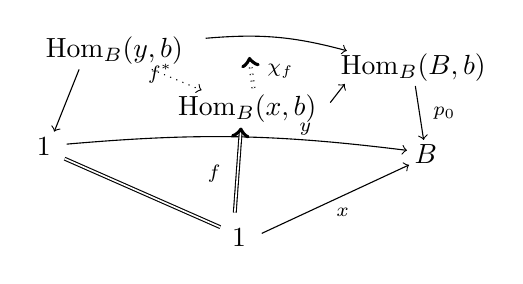
\begin{tikzpicture}[x=1.5em,y=1.5em]
  \node (Ey) at (0,3.3) {$\mathrm{Hom}_{B}(y,b)$};
  \node (E)  at (7.2,2.9) {$\mathrm{Hom}_{B}(B,b)$};
  \node (Ex) at (3.2,1.9) {$\mathrm{Hom}_{B}(x,b)$};
  \node (o1) at (-1.7,1.0) {$1$};
  \node (Bt) at (7.5,0.8) {$B$};
  \node (o2) at (3.0,-1.2) {$1$};
  \draw[->] (2.2,3.6) to[bend left=10] (5.6,3.3);
  \draw[->] (5.2,2.05) -- (5.55,2.5);
  \draw[->,dotted] (0.9,2.85) -- (2.1,2.35);
  \node at (1.1,2.75) {$\scriptstyle f^{*}$};
  \node at (1.55,3.0) {$\scriptstyle\llcorner$};
  \draw[double,->,dotted] (3.35,2.4) -- (3.25,3.15);
  \node at (4.0,2.8) {$\scriptstyle\chi_{f}$};
  \draw[->] (-0.85,2.85) -- (-1.45,1.35);
  \draw[->] (7.25,2.45) -- (7.45,1.15);
  \node at (7.95,1.8) {$\scriptstyle p_{0}$};
  \draw[->] (-1.15,1.05) to[bend left=6] (7.05,0.9);
  \node at (4.6,1.4) {$\scriptstyle y$};
  \node at (5.1,1.25) {$\scriptstyle\llcorner$};
  \draw[->] (3.55,-1.1) -- (7.1,0.55);
  \node at (5.5,-0.6) {$\scriptstyle x$};
  \draw[double] (-1.2,0.7) -- (2.55,-0.95);
  \draw[double,->] (2.9,-0.6) -- (3.05,1.45);
  \node at (2.4,0.35) {$\scriptstyle f$};
\end{tikzpicture}
\end{center}

粗略地说，一条\trIsofibration{} $p\colon E\to B$ 定义一个%
\emph{\trCartesianFibration}，恰在 $B$ 中的诸箭头以反变的函子性方式作用于其诸%
\trFiber{}之时；而定义一个\emph{\trCocartesianFibration}，则恰在这些箭头以协变的函子性
方式作用于诸\trFiber{}之时。\trFunctor{}
$p_{0}\colon\mathrm{Hom}_{B}(B,b)\twoheadrightarrow B$
便是一个\emph{\trDiscreteCartesianFibration}的例子，其诸\trFiber{}皆为%
\trDiscrete{}\trInfinityCategory。当 $b\colon X\to B$
是一个\trGeneralizedElement{}时，定义域投影\trFunctor{}
$p_{0}\colon\mathrm{Hom}_{B}(B,b)\to B$ 仍是一个\trCartesianFibration，但
失去了这一离散性。

刻画\trCartesianFibration{} $p\colon E\to B$ 的诸性质之中，有如下一条公理：
对任何以 $B$ 为余定义域的 2-\trCell{}，若其靶 1-\trCell{}的提升已指定，则存在
一个提升后的 2-\trCell{}，以 $E$ 为余定义域、以该 1-\trCell{}为靶。特别地，
在如下情形中这条提升性质便可施用：所论的 2-\trCell{}是\trHomotopyCategory{}
$\mathrm{h}B$ 中一支箭头的\trWhiskering（如下左所示），而源 1-\trCell{}的提升是其余
定义域之上\trFiber{}的典范包含：
\begin{rveq}\label{eq:cartesian-action}
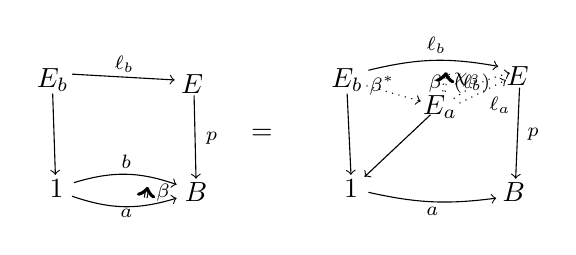
\begin{tikzpicture}[x=1.4em,y=1.4em]
  \node (Eb) at (0,2.1) {$E_{b}$};
  \node (El) at (3.6,2.0) {$E$};
  \node (oa) at (0.1,-0.7) {$1$};
  \node (Ba) at (3.7,-0.8) {$B$};
  \draw[->] (0.5,2.25) -- (3.15,2.1);
  \node at (1.85,2.5) {$\scriptstyle\ell_{b}$};
  \node at (0.8,1.95) {$\scriptstyle\llcorner$};
  \draw[->] (0.0,1.75) -- (0.07,-0.35);
  \draw[->] (3.65,1.7) -- (3.7,-0.45);
  \node at (4.1,0.6) {$\scriptstyle p$};
  \draw[->] (0.55,-0.55) to[bend left=18] (3.2,-0.6);
  \node at (1.9,0.0) {$\scriptstyle b$};
  \draw[double,->] (2.4,-0.94) -- (2.45,-0.66);
  \node at (2.85,-0.82) {$\scriptstyle\beta$};
  \draw[->] (0.5,-0.9) to[bend right=18] (3.2,-0.95);
  \node at (1.9,-1.35) {$\scriptstyle a$};
  \node at (5.4,0.7) {$=$};
  \node (Ebr) at (7.6,2.1) {$E_{b}$};
  \node (Ear) at (10.0,1.4) {$E_{a}$};
  \node (Er) at (12.0,2.2) {$E$};
  \node (ob) at (7.7,-0.7) {$1$};
  \node (Bb) at (11.9,-0.8) {$B$};
  \draw[->] (8.15,2.35) to[bend left=12] (11.5,2.45);
  \node at (9.9,3.0) {$\scriptstyle\ell_{b}$};
  \draw[double,->,dotted] (10.1,1.8) -- (10.15,2.3);
  \node at (10.7,2.1) {$\scriptstyle\chi_{\beta}$};
  \draw[->,dotted] (8.1,1.95) -- (9.5,1.55);
  \node at (8.5,1.95) {$\scriptstyle\beta^{*}$};
  \draw[->,dotted] (10.5,1.5) -- (11.7,2.1);
  \node at (11.55,1.45) {$\scriptstyle\ell_{a}$};
  \draw[->,dotted] (10.35,1.62) to[bend left=10] (11.8,2.28);
  \node at (10.5,2.02) {$\scriptstyle\beta^{*}(\ell_{b})$};
  \node at (10.3,1.15) {$\scriptstyle\llcorner$};
  \draw[->] (9.75,1.2) -- (8.05,-0.4);
  \draw[->] (7.6,1.75) -- (7.7,-0.35);
  \draw[->] (12.05,1.9) -- (11.95,-0.45);
  \node at (12.4,0.7) {$\scriptstyle p$};
  \draw[->] (8.15,-0.8) to[bend right=10] (11.45,-0.95);
  \node at (9.8,-1.3) {$\scriptstyle a$};
\end{tikzpicture}
\end{rveq}
此时，右方所示提升后的胞腔 $\chi_{\beta}$ 的定义域 $\beta^{*}(\ell_{b})$\footnote{原书
正文印作 $\beta^{*}(\ell_{a})$，其 (5.0.1) 图内标签及 5.2 节注 5.2.7 同类句均作
$\beta^{*}(\ell_{b})$，据图与后文径改。——译者注}严格
位于原 2-\trCell{}之余定义域的上方，因而穿过定义其\trFiber{}的那个\trPullback{}%
而分解。这就定义了一个\trFunctor{} $\beta^{*}\colon E_{b}\to E_{a}$，即箭头
$\beta$ 在 $p$ 的诸\trFiber{}上的「作用」。这一作用并非严格的，而是在同构意义
下函子性的，练习 5.2.ii 探讨了这一意义。\footnote{实情远不止此：还存在一个
反变的\trHomotopy{}相干\trDiagram{}，其标号为 $B$ 的\trUnderlyingQuasiCategory{}、
取值于诸\trDiscrete{}\trInfinityCategory{}的\trKanComplex{}富集范畴
[111, 6.1.16]。}这些作用映射在同构意义下的函子性，源自对指定的提升
2-\trCell{}所要求的一条\trUniversalProperty——它们正是我们将在 5.1 节中定义
的\emph{\trCartesianArrow}。

\trCartesianFibration{}将在 5.2 节中引入，最初的一批例子也在该节中确立。该节的
主定理借助某些典范定义的\trFunctor{}之\trAdjunction{}的存在来刻画%
\trCartesianFibration。\trCartesianFibration{}之间的保结构映射，是称为%
\emph{\trCartesianFunctor}的交换方块，它们保持诸笛卡尔自然变换。在 5.3 节中我们将看到，
相对于 5.2 节中构造的那些\trAdjunction{}，这些\trCartesianFunctor{}也能得到类似的刻画。

在 5.4 节中，我们研究对偶的\trCocartesianFibration，对此类纤维化而言，存在对%
\trNaturalTransformation{}的提升，且定义域\trFunctor{}已指定。由
\eqref{eq:cartesian-action} 所展示构造的一个对偶：当
$p\colon E\twoheadrightarrow B$ 是一条\trCocartesianFibration{}时，$\mathrm{h}B$ 中一支
箭头 $\beta\colon a\to b$ 定义出一个\trFunctor{} $\beta_{*}\colon E_{a}\to E_{b}$。
同时是\trCartesianFibration{}与\trCocartesianFibration{}的那条\trIsofibration{} $p$ 称为
一个\emph{\trBifibration}。\footnote{在 [78, \S2.4.7] 中，Lurie 用「bifibration」
一词指称另外一类函子：即第 7 章中的诸\trModule{}。}在此情形，命题 5.4.7 证明：
诱导出的诸\trFunctor{} $\beta_{*}\dashv\beta^{*}$ 构成\trAdjunction。

在 5.6 节中，我们将证明：当 $p\colon E\twoheadrightarrow B$
是一个\trInfinityCosmos{}中的\trCartesianFibration{}时，诱导\trFunctor{}
$p_{*}\colon\mathrm{Fun}(X,E)\twoheadrightarrow\mathrm{Fun}(X,B)$
定义出诸\trQuasiCategory{}的一个\trCartesianFibration；并且在附加条件——沿
任何 $f\colon Y\to X$ 的限制定义一个\trCartesianFunctor——之下，其逆亦真。

\emph{\trDiscreteCartesianFibration}与\emph{\trDiscreteCocartesianFibration}这两个特殊的类，将在 5.5 节
中得到研究。本章将在 5.7 节以\trYonedaLemma{}的一个版本作结，该版本针对的正是
由\trElement{} $b\colon 1\to B$ 所表示的那个\trDiscreteCartesianFibration
$p_{0}\colon\mathrm{Hom}_{B}(B,b)\twoheadrightarrow B$。其表述受到 Street 的
论文 \emph{Fibrations and Yoneda's lemma in a 2-category}
[118]\footnote{与 Street 的\trYonedaLemma{} [118, 16] 最接近的类比，出现于
定理 7.4.8。}的启发；这份承惠，我们在本节的标题中予以致谢。

\providecommand{\qcOne}{\mathbf{1}}   %
\providecommand{\qcTwo}{\mathbf{2}}   %
\providecommand{\qcThree}{\mathbf{3}} %
\providecommand{\qcFour}{\mathbf{4}}  %
\providecommand{\qcor}[1]{\ulcorner#1\urcorner}   %
\providecommand{\cellpair}[5]{$\vcenter{\hbox{\begin{tikzpicture}[x=1.15em,y=1.15em]%
\node (s) at (0,0) {$#1$};%
\node (t) at (4.2,0) {$#2$};%
\draw[->] (0.75,0.32) to[bend left=18] (3.45,0.32);%
\node at (2.1,0.88) {$\scriptstyle#3$};%
\draw[->] (0.75,-0.32) to[bend right=18] (3.45,-0.32);%
\node at (2.1,-0.93) {$\scriptstyle#4$};%
\draw[->] (1.95,0.2) to[bend right=32] (1.95,-0.2);%
\node at (2.85,0) {$\scriptstyle#5$};%
\end{tikzpicture}}}$\ignorespaces}

\section{笛卡尔箭头}\label{sec:cartesian-arrows}

在定义\textbf{\trCartesianFibration}（cartesian fibration）这一概念之前，我们先来
描述某些「楼上」的%
\trNaturalTransformation{}所享有的弱\trUniversalProperty。回忆：由第 3 章中的%
\cref{prop:arrow-category-uniqueness}，任何形如下式的\trNaturalTransformation{}
\cellpair{X}{E}{e'}{e}{\psi}
都由一个\trFunctor{} $\qcor{\psi}\colon X\to E^{2}$ 所表示，满足 $p_{0}\qcor{\psi}=e'$
与 $p_{1}\qcor{\psi}=e$，并且诸表示在\trFiberedIsomorphism{}之下唯一。$E$ 中这个%
表示性的 $X$-形箭头 $\qcor{\psi}$ 在\trFunctorSpace{} $\mathrm{Fun}(X,E)$ 中定义了%
一条从 $e'$ 到 $e$ 的 1-箭头（亦称 1-\trSimplex）。

\begin{definition}[$p$-笛卡尔箭头]\label{def:pcartesian-arrow}
设 $p\colon E\twoheadrightarrow B$ 为一条\trIsofibration。$E$ 中的一条 $X$-形箭头%
$\qcor{\psi}\colon X\to E^{2}$ 是\textbf{$p$-\trCartesian}，若由%
\trLeibnizCotensor{}的\trPullback{}所定义的虚线映射是一条\trTrivialFibration：
\begin{center}
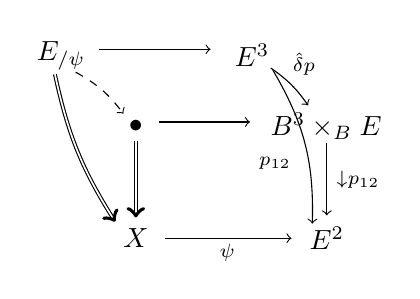
\begin{tikzpicture}[x=1.5em,y=1.5em]
  \node (Ep) at (0,2.7) {$E_{/\psi}$};
  \node (E3) at (4.6,2.7) {$E^{3}$};
  \node (dt) at (1.8,1.0) {$\bullet$};
  \node (BB) at (6.4,1.0) {$B^{3}\times_{B^{\llcorner}}E^{\llcorner}$};
  \node (X)  at (1.8,-1.7) {$X$};
  \node (E2) at (6.4,-1.7) {$E^{2}$};
  \draw[->] (0.9,2.85) -- (3.6,2.85);
  \node at (2.25,3.15) {$\scriptstyle\llcorner$};
  \draw[->,dashed] (0.35,2.3) to[bend left=12] (1.5,1.3);
  \draw[->] (2.35,1.1) -- (4.55,1.1);
  \node at (3.45,1.4) {$\scriptstyle\llcorner$};
  \draw[->] (5.05,2.4) to[bend left=10] (5.95,1.5);
  \node at (5.85,2.5) {$\scriptstyle\hat{\delta}p$};
  \draw[->] (6.4,0.6) -- (6.4,-1.15);
  \node at (7.15,-0.3) {$\scriptstyle\downarrow p_{12}$};
  \draw[->] (5.1,2.35) to[bend left=16] (6.05,-1.35);
  \node at (5.15,0.1) {$\scriptstyle p_{12}$};
  \draw[double,->] (-0.15,2.25) to[bend right=10] (1.3,-1.3);
  \draw[double,->] (1.8,0.65) -- (1.8,-1.2);
  \draw[->] (2.5,-1.7) -- (5.55,-1.7);
  \node at (4.0,-2.05) {$\scriptstyle\qcor{\psi}$};
\end{tikzpicture}
\end{center}
其中 $\delta\colon\llcorner\hookrightarrow\qcThree$是其像为 $\qcThree$ 中%
\trCospan{} $0\to 2\leftarrow 1$ 的那个包含，而 $p_{12}$ 定义为沿包含%
$i_{12}\colon\qcTwo\hookrightarrow\qcThree$的限制，其像即下标所示。
\end{definition}

余定义域为 $E$ 的一条\trNaturalTransformation{}
\cellpair{X}{E}{e'}{e}{\psi}
是 $p$-\trCartesian，若表示它的每一个\trFunctor{} $\qcor{\psi}\colon X\to E^{2}$
都是 $p$-\trCartesian。由练习 3.3.i，这一说法是良定的。我们将在\trNaturalTransformation{}%
$\psi\colon e'\Rightarrow e$ 所呈现的视角与表示箭头 $\qcor{\psi}\colon X\to E^{2}$
所呈现的视角之间自由切换。\footnote{我们也沿用一套精简记号：把警告 4.2.10 中以记号%
$E_{/\qcor{\psi}}$定义的\trInfinityCategory{}径写作 $E_{/\psi}$，并把复合箭头%
$p^{2}\qcor{\psi}$与 $\qcor{\psi}f$分别写作 $\qcor{p^{2}\psi}$与 $\qcor{\psi f}$。}
存在多种彼此等价的方式来陈述 $p$-笛卡尔箭头的定义。

\begin{lemma}\label{lem:dashed-square-hypercube}
对任意\trIsofibration{} $p\colon E\twoheadrightarrow B$，余定义域为%
$e\colon X\to E$的一支箭头 $\qcor{\psi}\colon X\to E^{2}$ 是 $p$-\trCartesian，
当且仅当由超立方体
\begin{rveq}\label{eq:hypercube-weakly-cartesian}
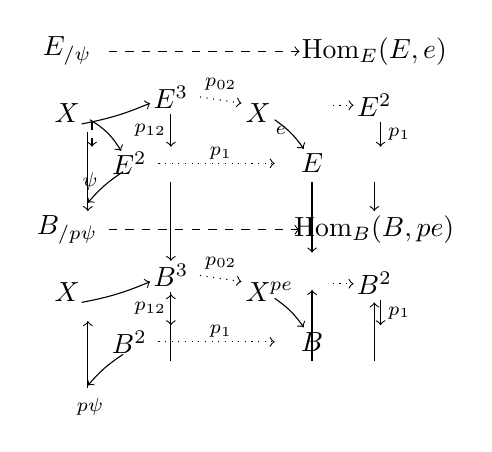
\begin{tikzpicture}[x=1.5em,y=1.5em]
  \node (Ep) at (0,5.2) {$E_{/\psi}$};
  \node (HE) at (7.4,5.2) {$\mathrm{Hom}_{E}(E,e)$};
  \draw[->,dashed] (1.0,5.2) -- (5.6,5.2);
  \node (Xa) at (0,3.7) {$X$};
  \node (E3) at (2.5,4.1) {$E^{3}$};
  \node (Xb) at (4.6,3.7) {$X$};
  \node (E2a) at (7.4,3.9) {$E^{2}$};
  \node (E2b) at (1.5,2.5) {$E^{2}$};
  \node (Eob) at (5.9,2.5) {$E$};
  \draw[->] (0.35,3.45) to[bend right=6] (2.0,3.95);
  \draw[->,dashed] (0.6,3.5) -- (0.6,2.9);
  \draw[->] (0.55,3.55) to[bend left=14] (1.3,2.8);
  \draw[->,dotted] (3.2,4.1) -- node[above]{$\scriptstyle p_{02}$} (4.2,3.95);
  \draw[->,dotted] (6.4,3.9) -- (6.9,3.9);
  \draw[->] (5.0,3.55) to[bend left=10] (5.7,2.85);
  \node at (5.15,3.3) {$\scriptstyle e$};
  \draw[->] (7.55,3.5) -- (7.55,2.9);
  \node at (8.0,3.2) {$\scriptstyle p_{1}$};
  \draw[->] (2.5,3.7) -- (2.5,2.9);
  \node at (2.0,3.3) {$\scriptstyle p_{12}$};
  \draw[->,dotted] (2.2,2.5) -- (5.0,2.5);
  \node at (3.7,2.75) {$\scriptstyle p_{1}$};
  \draw[->] (1.35,2.3) to[bend right=8] (0.5,1.55);
  \node at (0.55,2.05) {$\scriptstyle\qcor{\psi}$};
  \node (Bp) at (0,0.9) {$B_{/p\psi}$};
  \node (HB) at (7.4,0.9) {$\mathrm{Hom}_{B}(B,pe)$};
  \draw[->,dashed] (1.0,0.9) -- (5.6,0.9);
  \node (Xc) at (0,-0.6) {$X$};
  \node (B3) at (2.5,-0.2) {$B^{3}$};
  \node (Xd) at (4.6,-0.6) {$X$};
  \node (B2a) at (7.4,-0.4) {$B^{2}$};
  \node (B2b) at (1.5,-1.8) {$B^{2}$};
  \node (Bb) at (5.9,-1.8) {$B$};
  \draw[->] (0.35,-0.85) to[bend right=6] (2.0,-0.35);
  \draw[->,dotted] (3.2,-0.2) -- node[above]{$\scriptstyle p_{02}$} (4.2,-0.35);
  \draw[->,dotted] (6.4,-0.4) -- (6.9,-0.4);
  \draw[->] (5.0,-0.75) to[bend left=10] (5.7,-1.45);
  \node at (5.15,-0.5) {$\scriptstyle pe$};
  \draw[->] (7.55,-0.8) -- (7.55,-1.4);
  \node at (8.0,-1.1) {$\scriptstyle p_{1}$};
  \draw[->] (2.5,-0.6) -- (2.5,-1.4);
  \node at (2.0,-1.0) {$\scriptstyle p_{12}$};
  \draw[->,dotted] (2.2,-1.8) -- (5.0,-1.8);
  \node at (3.7,-1.55) {$\scriptstyle p_{1}$};
  \draw[->] (1.35,-2.1) to[bend right=8] (0.5,-2.85);
  \node at (0.55,-3.35) {$\scriptstyle\qcor{p\psi}$};
  \draw[->] (0.5,-2.9) -- (0.5,-1.3);
  \draw[->] (2.5,-2.25) -- (2.5,-0.65);
  \draw[->] (5.9,-2.25) -- (5.9,-0.55);
  \draw[->] (7.4,-2.25) -- (7.4,-0.85);
  \draw[->] (0.5,3.25) -- (0.5,1.35);
  \draw[->] (2.5,2.05) -- (2.5,0.15);
  \draw[->] (5.9,2.05) -- (5.9,0.35);
  \draw[->] (7.4,2.05) -- (7.4,1.35);
\end{tikzpicture}
\end{rveq}
所诱导的虚线方块是\trWeaklyCartesianSquare，也就是说，其诱导映射是一条%
\trTrivialFibration：
\[
E_{/\psi}\rightsquigarrow B_{/p\psi}\times_{\mathrm{Hom}_{B}(B,pe)}\mathrm{Hom}_{E}(E,e)
\]
\end{lemma}

\begin{proof}
事实上，虚线方块中诱导出的映射与\cref{def:pcartesian-arrow} 的映射同构。首先注意，%
超立方体 \eqref{eq:hypercube-weakly-cartesian} 中的实线方块都是\trPullback，故由%
超立方体拉回引理\footnote{超立方体拉回引理说的是：形如 $\llcorner\times\llcorner$
的\trDiagram{}的极限，既可先取左因子的诸\trPullback{}再对所得\trCospan{}取%
\trPullback{}而算得，也可先取右因子的诸\trPullback{}再对所得\trCospan{}取%
\trPullback{}而算得。}，虚线方块中的\trPullback{}同样等于图表
\begin{center}
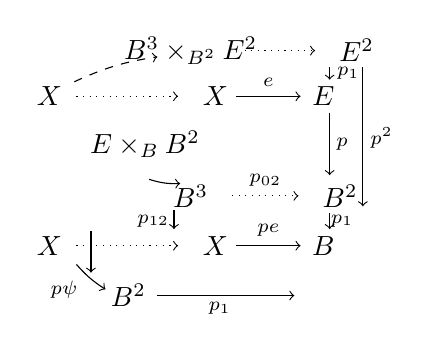
\begin{tikzpicture}[x=1.5em,y=1.5em]
  \node (BE2) at (3.4,2.6) {$B^{3}\times_{B^{2}}E^{2}$};
  \node (E2t) at (7.4,2.6) {$E^{2}$};
  \draw[->,dotted] (4.7,2.6) -- (6.4,2.6);
  \node (Xa) at (0,1.5) {$X$};
  \node (Xb) at (4.0,1.5) {$X$};
  \node (E)   at (6.6,1.5) {$E$};
  \draw[->,dashed] (0.6,1.85) to[bend left=8] (2.6,2.45);
  \draw[->,dotted] (0.65,1.5) -- (3.1,1.5);
  \draw[->] (4.5,1.5) -- node[above]{$\scriptstyle e$} (6.05,1.5);
  \node (EB2) at (2.3,0.35) {$E\times_{B}B^{2}$};
  \draw[->] (6.75,2.2) -- (6.75,1.9);
  \node at (7.2,2.05) {$\scriptstyle p_{1}$};
  \draw[->] (7.55,2.2) -- (7.55,-1.15);
  \node at (8.0,0.5) {$\scriptstyle p^{2}$};
  \draw[->] (6.75,1.1) -- (6.75,-0.4);
  \node at (7.05,0.35) {$\scriptstyle p$};
  \node (B3) at (3.4,-0.9) {$B^{3}$};
  \node (B2t) at (7.0,-0.9) {$B^{2}$};
  \draw[->,dotted] (4.4,-0.9) -- node[above]{$\scriptstyle p_{02}$} (6.0,-0.9);
  \node (Xc) at (0,-2.1) {$X$};
  \node (Xd) at (4.0,-2.1) {$X$};
  \node (B)  at (6.6,-2.1) {$B$};
  \draw[->,dotted] (0.65,-2.1) -- (3.1,-2.1);
  \draw[->] (4.5,-2.1) -- node[above]{$\scriptstyle pe$} (6.05,-2.1);
  \node (B2b) at (1.9,-3.3) {$B^{2}$};
  \draw[->] (1.0,-1.75) -- (1.0,-2.75);
  \draw[->] (0.65,-2.55) to[bend right=8] (1.35,-3.15);
  \node at (0.35,-3.15) {$\scriptstyle\qcor{p\psi}$};
  \draw[->] (2.6,-3.3) -- (5.9,-3.3);
  \node at (4.1,-3.6) {$\scriptstyle p_{1}$};
  \draw[->] (6.75,-1.3) -- (6.75,-1.7);
  \node at (7.05,-1.5) {$\scriptstyle p_{1}$};
  \draw[->] (2.4,-0.5) to[bend right=10] (3.15,-0.6);
  \draw[->] (3.0,-1.25) -- (3.0,-1.7);
  \node at (2.5,-1.5) {$\scriptstyle p_{12}$};
\end{tikzpicture}
\end{center}
的极限，其中此时点线方块是\trPullback。于是，我们的映射同构于某立方体的顶部虚映射%
——该立方体的前面与后面恰是定义其定义域与余定义域的诸\trPullback：
\begin{center}
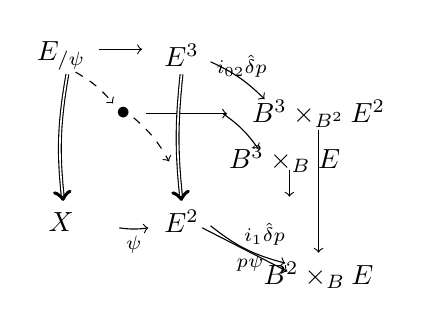
\begin{tikzpicture}[x=1.5em,y=1.5em]
  \node (Ep) at (0,2.4) {$E_{/\psi}$};
  \node (E3) at (2.9,2.4) {$E^{3}$};
  \node (dt) at (1.5,1.0) {$\bullet$};
  \node (BB) at (6.2,1.0) {$B^{3}\times_{B^{2}}E^{2}$};
  \node (mB) at (5.4,-0.1) {$B^{3}\times_{B^{\llcorner}}E^{\llcorner}$};
  \node (X)  at (0,-1.6) {$X$};
  \node (E2) at (2.9,-1.6) {$E^{2}$};
  \node (BX) at (6.2,-2.9) {$B^{2}\times_{B}E$};
  \draw[->] (0.9,2.55) -- (1.95,2.55);
  \node at (1.4,2.85) {$\scriptstyle\llcorner$};
  \draw[->] (3.6,2.25) to[bend left=10] (4.9,1.35);
  \node at (4.35,2.15) {$\scriptstyle i_{02}\hat{\delta}p$};
  \draw[->,dashed] (0.35,2.0) to[bend left=10] (1.25,1.25);
  \draw[->,dashed] (1.75,0.9) to[bend left=10] (2.6,-0.15);
  \draw[->] (2.05,1.0) -- (4.0,1.0);
  \node at (3.0,1.3) {$\scriptstyle\llcorner$};
  \draw[->] (3.9,1.0) to[bend left=10] (4.75,0.15);
  \node at (4.6,0.72) {$\scriptstyle\llcorner$};
  \draw[->] (5.5,-0.35) -- (5.5,-1.0);
  \node at (6.05,-0.7) {$\scriptstyle\llcorner$};
  \draw[->] (6.2,0.6) -- (6.2,-2.35);
  \draw[->] (1.4,-1.75) to[bend right=8] (2.1,-1.75);
  \node at (1.75,-2.15) {$\scriptstyle\qcor{\psi}$};
  \draw[->] (3.6,-1.7) to[bend right=12] (5.4,-2.6);
  \node at (4.9,-1.9) {$\scriptstyle i_{1}\hat{\delta}p$};
  \draw[->] (3.4,-1.75) -- (5.45,-2.8);
  \node at (4.55,-2.6) {$\scriptstyle\qcor{p\psi}$};
  \draw[double,->] (0.15,1.95) to[bend right=8] (0.05,-1.1);
  \draw[double,->] (2.9,1.95) to[bend right=6] (2.9,-1.1);
\end{tikzpicture}
\end{center}
到右面中\trPullback{}的诱导映射是 $\hat{\delta}p\colon E^{3}\to B^{3}\times_{B^{\llcorner}}E^{\llcorner}$，
这可以通过再构造一个超立方体来验证。由\trPullback{}的复合与消去，此映射经拉回即得%
左面中的虚映射；但由于底边是恒同，它与顶部虚映射重合。注意，%
\cref{def:pcartesian-arrow}中展示的图表作为后棱柱嵌入在这个立方体中。
\end{proof}

接下来的几条引理将为相对于固定\trIsofibration{} $p\colon E\twoheadrightarrow B$
而定义的 $p$-笛卡尔变换类发展出若干稳定性性质。

\begin{lemma}[限制下的稳定性]\label{lem:stability-under-restriction}
若 $\qcor{\psi}\colon X\to E^{2}$ 是 $p$-\trCartesian，则它沿任何\trFunctor{}%
$f\colon Y\to X$的限制亦然。
\end{lemma}

\begin{proof}
由\cref{def:pcartesian-arrow}，若 $\psi$ 是 $p$-\trCartesian，我们便有一条%
\trTrivialFibration
\begin{center}
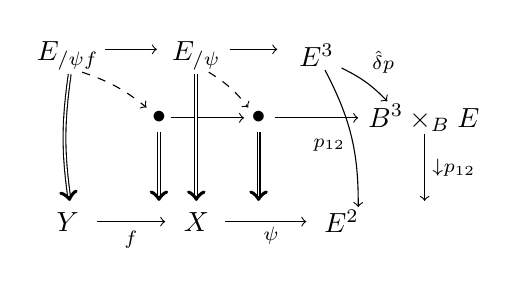
\begin{tikzpicture}[x=1.5em,y=1.5em]
  \node (Epf) at (0,2.5) {$E_{/\psi f}$};
  \node (Ep)  at (3.1,2.5) {$E_{/\psi}$};
  \node (E3)  at (6.0,2.5) {$E^{3}$};
  \node (d1)  at (2.2,1.0) {$\bullet$};
  \node (d2)  at (4.6,1.0) {$\bullet$};
  \node (BB)  at (8.6,1.0) {$B^{3}\times_{B^{\llcorner}}E^{\llcorner}$};
  \node (Y)   at (0,-1.5) {$Y$};
  \node (X)   at (3.1,-1.5) {$X$};
  \node (E2)  at (6.6,-1.5) {$E^{2}$};
  \draw[->] (0.9,2.65) -- (2.15,2.65);
  \node at (1.5,2.95) {$\scriptstyle\llcorner$};
  \draw[->] (3.9,2.65) -- (5.05,2.65);
  \node at (4.5,2.95) {$\scriptstyle\llcorner$};
  \draw[->] (6.6,2.2) to[bend left=10] (7.7,1.4);
  \node at (7.6,2.35) {$\scriptstyle\hat{\delta}p$};
  \draw[->,dashed] (0.35,2.1) to[bend left=10] (1.9,1.25);
  \draw[->,dashed] (3.4,2.1) to[bend left=10] (4.35,1.25);
  \draw[->] (2.5,1.0) -- (4.25,1.0);
  \node at (3.4,1.3) {$\scriptstyle\llcorner$};
  \draw[->] (5.0,1.0) -- (7.0,1.0);
  \node at (6.0,1.3) {$\scriptstyle\llcorner$};
  \draw[->] (8.6,0.6) -- (8.6,-1.0);
  \node at (9.3,-0.2) {$\scriptstyle\downarrow p_{12}$};
  \draw[->] (6.2,2.15) to[bend left=14] (7.0,-1.15);
  \node at (6.3,0.35) {$\scriptstyle p_{12}$};
  \draw[double,->] (0.05,2.05) to[bend right=8] (0.05,-1.0);
  \draw[double,->] (3.1,2.05) -- (3.1,-1.0);
  \draw[double,->] (2.2,0.65) -- (2.2,-1.0);
  \draw[double,->] (4.6,0.65) -- (4.6,-1.0);
  \draw[->] (0.7,-1.5) -- node[below]{$\scriptstyle f$} (2.35,-1.5);
  \draw[->] (3.8,-1.5) -- (5.75,-1.5);
  \node at (4.9,-1.85) {$\scriptstyle\qcor{\psi}$};
\end{tikzpicture}
\end{center}
它经拉回定义出一条\trTrivialFibration，后者表明 $\qcor{\psi f}$ 是一支%
$p$-\trCartesian{}箭头。
\end{proof}

我们现在来证明：$p$-笛卡尔变换类在\trHomotopyTwoCategory{}中对竖复合与左消去封闭。

\begin{lemma}\label{lem:left-cancellation}
设 $p\colon E\twoheadrightarrow B$ 为\trIsofibration，并考虑满足%
$\psi''=\psi\cdot\psi'$的一些\trNaturalTransformation，其中 $\psi$ 是%
$p$-\trCartesian。则 $\psi'$ 是 $p$-\trCartesian，当且仅当 $\psi''$ 是%
$p$-\trCartesian。
\end{lemma}

\begin{proof}
由第 1 章中的引理 1.1.12，对任意代表满足 $\psi''=\psi\cdot\psi'$的%
\trNaturalTransformation{}的三支箭头 $\qcor{\psi''}$、$\qcor{\psi'}$、%
$\qcor{\psi}\colon X\to E^{3}$，存在 $\mathrm{Fun}(X,E)$ 中的一个%
2-\trSimplex，它由一个\trFunctor{} $\qcor{\tau}\colon X\to E^{3}$ 所表示，
其边界恰由这些指定的表示函子给出：
\begin{center}
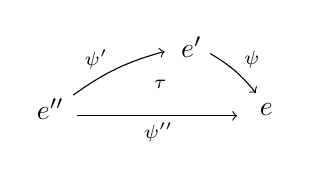
\begin{tikzpicture}[x=1.5em,y=1.5em]
  \node (epp) at (0,0) {$e''$};
  \node (ep)  at (3.4,1.5) {$e'$};
  \node (e)   at (5.2,0) {$e$};
  \draw[->] (0.55,0.35) to[bend left=10] (2.75,1.4);
  \node at (1.1,1.2) {$\scriptstyle\psi'$};
  \draw[->] (3.85,1.35) to[bend left=10] (4.95,0.4);
  \node at (4.85,1.2) {$\scriptstyle\psi$};
  \draw[->] (0.65,-0.15) -- (4.5,-0.15);
  \node at (2.6,-0.55) {$\scriptstyle\psi''$};
  \node at (2.65,0.6) {$\scriptstyle\tau$};
\end{tikzpicture}
\end{center}
通过把左下的范畴图表\trCotensor{}入 $E$、限制到始顶点 $0\in\qcOne$的补、再沿%
$\qcor{\tau}\colon X\to E^{3}$及其面拉回，我们得到右下的∞-范畴图表，其中底部%
方块是\trWeaklyCartesianSquare（关于外跨度之构造以及 $p_{01}$ 皆为%
\trTrivialFibration{}的证明，详见第 4 章中的引理 4.3.9）。
\begin{center}
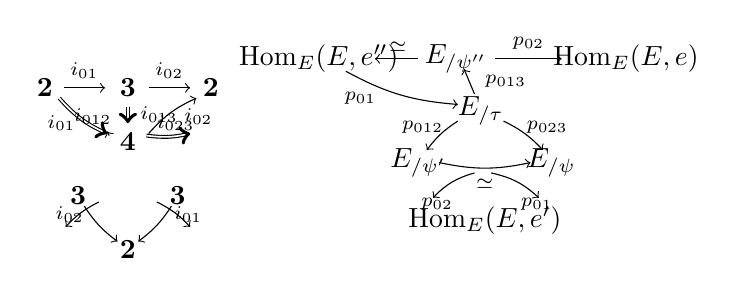
\begin{tikzpicture}[x=1.5em,y=1.5em]
  \node (t2a) at (0,2.2) {$\qcTwo$};
  \node (t3a) at (2.0,2.2) {$\qcThree$};
  \node (t2b) at (4.0,2.2) {$\qcTwo$};
  \draw[->] (0.45,2.2) -- node[above]{$\scriptstyle i_{01}$} (1.45,2.2);
  \draw[->] (2.5,2.2) -- node[above]{$\scriptstyle i_{02}$} (3.5,2.2);
  \node (t4) at (2.0,0.9) {$\qcFour$};
  \draw[double,->] (2.0,1.75) -- (2.0,1.35);
  \node at (2.75,1.55) {$\scriptstyle i_{013}$};
  \draw[double,->] (0.35,1.95) to[bend right=12] (1.5,1.1);
  \node at (0.4,1.35) {$\scriptstyle i_{01}$};
  \draw[->] (1.55,1.05) -- (1.5,1.15);
  \node at (1.15,1.5) {$\scriptstyle i_{012}$};
  \draw[->] (2.5,1.1) to[bend left=12] (3.65,1.95);
  \node at (3.7,1.5) {$\scriptstyle i_{02}$};
  \draw[double,->] (2.45,1.05) to[bend right=10] (3.5,1.1);
  \node at (3.15,1.35) {$\scriptstyle i_{023}$};
  \node (t3b) at (0.8,-0.4) {$\qcThree$};
  \node (t3c) at (3.2,-0.4) {$\qcThree$};
  \draw[->] (1.3,-0.55) to[bend right=10] (0.5,-1.15);
  \node at (0.6,-0.85) {$\scriptstyle i_{02}$};
  \draw[->] (2.7,-0.55) to[bend left=10] (3.5,-1.15);
  \node at (3.45,-0.85) {$\scriptstyle i_{01}$};
  \node (t2c) at (2.0,-1.7) {$\qcTwo$};
  \draw[->] (0.95,-0.65) to[bend right=10] (1.75,-1.5);
  \draw[->] (3.05,-0.65) to[bend left=10] (2.25,-1.5);
  \node at (5.5,0.4) {$\rightsquigarrow$};
  \begin{scope}[shift={(6.6,0.9)}]
  \node (HE2) at (0,2.0) {$\mathrm{Hom}_{E}(E,e'')$};
  \node (E2p) at (3.3,2.0) {$E_{/\psi''}$};
  \node (HE3) at (7.4,2.0) {$\mathrm{Hom}_{E}(E,e)$};
  \draw[->] (2.4,2.0) -- (1.35,2.0);
  \node at (1.9,2.3) {$\scriptstyle\simeq$};
  \draw[->] (4.25,2.0) -- node[above]{$\scriptstyle p_{02}$} (5.85,2.0);
  \node (Et) at (3.9,0.75) {$E_{/\tau}$};
  \draw[->] (3.75,1.15) -- (3.5,1.75);
  \node at (4.5,1.45) {$\scriptstyle p_{013}$};
  \node (Epp) at (2.4,-0.5) {$E_{/\psi'}$};
  \node (Eps) at (5.6,-0.5) {$E_{/\psi}$};
  \draw[->] (3.35,0.5) to[bend right=10] (2.6,-0.2);
  \node at (2.5,0.35) {$\scriptstyle p_{012}$};
  \draw[->] (4.45,0.5) to[bend left=10] (5.4,-0.2);
  \node at (5.5,0.35) {$\scriptstyle p_{023}$};
  \draw[->] (0.65,1.7) to[bend right=12] (3.35,0.9);
  \node at (1.0,1.05) {$\scriptstyle p_{01}$};
  \draw[->] (3.75,-0.75) to[bend right=15] (2.75,-1.35);
  \node at (2.85,-1.5) {$\scriptstyle p_{02}$};
  \draw[->] (4.15,-0.75) to[bend left=15] (5.3,-1.35);
  \node at (5.25,-1.5) {$\scriptstyle p_{01}$};
  \draw[->] (2.9,-0.5) to[bend right=12] (5.1,-0.5);
  \node at (4.0,-1.0) {$\scriptstyle\simeq$};
  \node (HE1) at (4.0,-1.9) {$\mathrm{Hom}_{E}(E,e')$};
  \end{scope}
\end{tikzpicture}
\end{center}
\trIsofibration{} $p\colon E\twoheadrightarrow B$定义了从这个图表到为%
$\qcor{p\tau}\colon X\to B^{3}$构造的类似图表的一个\trNaturalTransformation。%
\footnote{构造此图的更佳途径，是把这一构造实现在由第 6 章中的命题 6.1.1 定义的%
\trIsofibration\trInfinityCosmos{}中；这还额外告诉我们，每个自然性方块中到%
\trPullback{}的映射都是\trIsofibration。}
\cref{lem:dashed-square-hypercube}的\trTrivialFibration{}
$E_{/\psi}\twoheadrightarrow B_{/p\psi}\times_{\mathrm{Hom}_{B}(B,pe)}\mathrm{Hom}_{E}(E,e)$
经拉回定义出下图中展示的虚\trTrivialFibration，它与来自 $E_{/\tau}$ 的诱导映射交换：
\begin{center}
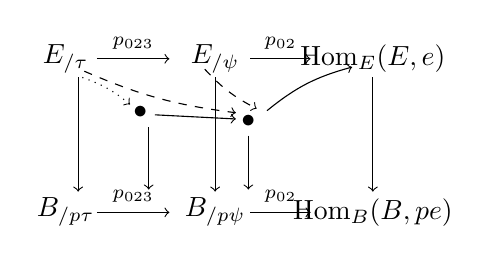
\begin{tikzpicture}[x=1.5em,y=1.5em]
  \node (Et) at (0,2.4) {$E_{/\tau}$};
  \node (Eps) at (3.6,2.4) {$E_{/\psi}$};
  \node (HE)  at (7.4,2.4) {$\mathrm{Hom}_{E}(E,e)$};
  \draw[->] (0.75,2.4) -- node[above]{$\scriptstyle p_{023}$} (2.5,2.4);
  \draw[->] (4.45,2.4) -- node[above]{$\scriptstyle p_{02}$} (5.9,2.4);
  \node (d1) at (1.8,1.1) {$\bullet$};
  \node (d2) at (4.4,0.9) {$\bullet$};
  \draw[->,dotted] (0.4,1.95) to[bend left=10] (1.55,1.3);
  \draw[->,dashed] (0.45,2.1) to[bend right=8] (4.1,1.1);
  \draw[->,dashed] (3.35,2.15) to[bend right=10] (4.6,1.2);
  \draw[->] (2.15,1.05) -- (4.1,0.95);
  \node at (3.1,1.3) {$\scriptstyle\llcorner$};
  \draw[->] (4.85,1.15) to[bend left=12] (6.9,2.2);
  \node at (5.7,1.4) {$\scriptstyle\llcorner$};
  \node (Bpt) at (0,-1.3) {$B_{/p\tau}$};
  \node (Bps) at (3.6,-1.3) {$B_{/p\psi}$};
  \node (HB)  at (7.4,-1.3) {$\mathrm{Hom}_{B}(B,pe)$};
  \draw[->] (0.75,-1.3) -- node[above]{$\scriptstyle p_{023}$} (2.5,-1.3);
  \draw[->] (4.45,-1.3) -- node[above]{$\scriptstyle p_{02}$} (5.9,-1.3);
  \draw[->] (0.3,1.95) -- (0.3,-0.8);
  \draw[->] (3.6,1.95) -- (3.6,-0.8);
  \draw[->] (7.4,1.95) -- (7.4,-0.8);
  \draw[->] (2.0,0.75) -- (2.0,-0.75);
  \draw[->] (4.4,0.55) -- (4.4,-0.75);
\end{tikzpicture}
\end{center}
由等价的\trTwoOfThreeProperty，若两条点线映射中任一条是\trTrivialFibration，
则另一条亦是。
\end{proof}

这些图表诱导出一个交换方块，展示于立方体内部——从上方的点线映射指向检测%
$\psi'$是否 $p$-笛卡尔的那条映射：
\begin{center}
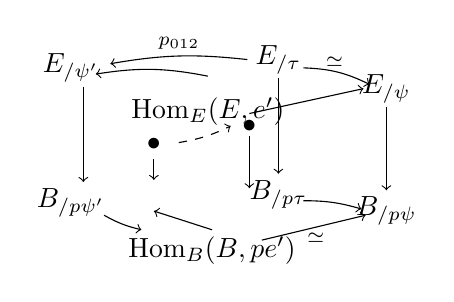
\begin{tikzpicture}[x=1.5em,y=1.5em]
  \node (Epp) at (0,2.4) {$E_{/\psi'}$};
  \node (Et)  at (5.0,2.6) {$E_{/\tau}$};
  \node (Eps) at (7.6,1.9) {$E_{/\psi}$};
  \draw[->] (4.25,2.6) to[bend right=8] (0.95,2.5);
  \node at (2.6,3.0) {$\scriptstyle p_{012}$};
  \draw[->] (5.6,2.4) to[bend left=12] (7.2,2.0);
  \node at (6.35,2.55) {$\scriptstyle\simeq$};
  \node (HE1) at (3.3,1.35) {$\mathrm{Hom}_{E}(E,e')$};
  \draw[->] (3.3,2.2) to[bend right=10] (0.6,2.25);
  \draw[->] (4.3,1.3) -- (7.05,1.9);
  \node at (4.3,1.0) {$\bullet$};
  \node at (2.0,0.55) {$\bullet$};
  \draw[->,dashed] (2.6,0.6) to[bend right=8] (3.85,1.0);
  \node at (3.2,1.05) {$\scriptstyle\rightsquigarrow$};
  \draw[->] (0.3,1.95) -- (0.3,-0.35);
  \draw[->] (5.0,2.15) -- (5.0,-0.15);
  \draw[->] (7.6,1.45) -- (7.6,-0.55);
  \node (Bpp) at (0,-0.85) {$B_{/p\psi'}$};
  \node (Bpt) at (5.0,-0.65) {$B_{/p\tau}$};
  \node (Bps) at (7.6,-1.05) {$B_{/p\psi}$};
  \draw[->] (0.8,-1.15) to[bend right=8] (1.7,-1.5);
  \draw[->] (5.6,-0.8) to[bend left=8] (7.0,-1.0);
  \node (HB1) at (3.4,-2.0) {$\mathrm{Hom}_{B}(B,pe')$};
  \draw[->] (3.4,-1.5) -- (2.0,-1.05);
  \draw[->] (4.6,-1.75) -- (7.1,-1.15);
  \node at (5.9,-1.7) {$\scriptstyle\simeq$};
  \draw[->] (2.0,0.2) -- (2.0,-0.3);
  \node at (1.55,-0.05) {$\scriptstyle\llcorner$};
  \draw[->] (4.3,0.75) -- (4.3,-0.5);
  \node at (3.85,0.1) {$\scriptstyle\llcorner$};
\end{tikzpicture}
\end{center}
由\trTwoOfThreeProperty，这两条映射中若有一条是\trTrivialFibration，另一条亦是。
用$p_{013}\colon E_{/\tau}\twoheadrightarrow E_{/\psi''}$定义的类似方块表明：下方点线%
映射是\trTrivialFibration，当且仅当%
$E_{/\psi''}\twoheadrightarrow B_{/p\psi''}\times_{\mathrm{Hom}_{B}(B,pe)}\mathrm{Hom}_{E}(E,e)$
是。于是，当 $\psi$ 是 $p$-\trCartesian{}时，这些条件彼此等价。

$p$-笛卡尔箭头的同构稳定性由下面这组观察来表达：

\begin{lemma}\label{lem:isomorphism-stability}
设 $p\colon E\twoheadrightarrow B$为\trIsofibration。
\begin{enumerate}[label=(\roman*)]
\item 余定义域为 $E$ 的自然同构定义 $p$-笛卡尔箭头。
\item 自然同构的任一 $p$-笛卡尔提升都是自然同构。
\item $p$-笛卡尔箭头类对与自然同构的\trPreComposition{}与\trPostComposition{}封闭。
\end{enumerate}
\end{lemma}

\begin{proof}
由第 4 章中的引理 4.3.9，$\psi\colon e'\Rightarrow e$是一个\trIsomorphism，
当且仅当定义\cref{lem:dashed-square-hypercube}中\trWeaklyCartesianSquare{}顶部%
水平箭头的映射 $p_{02}\colon E_{/\psi}\to\mathrm{Hom}_{E}(E,e)$是一条%
\trTrivialFibration。
于是若 $\psi$ 可逆，则\cref{lem:dashed-square-hypercube}的两条水平箭头都是%
\trTrivialFibration，该方块自动成为\trWeaklyCartesianSquare，这证明了 (i)。
对于 (ii)，若 $p\psi$ 可逆，则此方块中的底部水平箭头是\trTrivialFibration，
于是当 $\psi$ 是\trWeaklyCartesian{}时，%
$p_{02}\colon E_{/\psi}\to\mathrm{Hom}_{E}(E,e)$是诸\trTrivialFibration{}的%
一个复合，这证明 $\psi$ 可逆。最后的性质 (iii) 由 (i) 与%
\cref{lem:left-cancellation}得到。
\end{proof}

我们从 $p$-笛卡尔箭头的两种更为精细的刻画中获得相当可观的回报。

\begin{theorem}\label{thm:pcartesian-characterizations}
设 $p\colon E\twoheadrightarrow B$为\trIsofibration，$\qcor{\psi}\colon X\to E^{2}$
为表示\trNaturalTransformation{}
\cellpair{X}{E}{e'}{e}{\psi}
的一支箭头。下列诸条等价：
\begin{enumerate}[label=(\roman*)]
\item $\psi$ 是 $p$-\trCartesian。
\item 交换三角形定义出一个绝对右提升图表：
\begin{center}
\begin{tikzpicture}[x=1.5em,y=1.5em]
  \node (E2) at (3.2,1.5) {$E^{2}$};
  \node (X)  at (0,0) {$X$};
  \node (HB) at (3.2,0) {$\mathrm{Hom}_{B}(B,p)$};
  \draw[->] (0.55,0.4) -- node[above,pos=0.6]{$\scriptstyle\qcor{\psi}$} (2.5,1.3);
  \draw[->] (3.2,1.05) -- (3.2,0.45);
  \node at (3.95,0.75) {$\scriptstyle i_{1}\hat{\delta}p$};
  \draw[double,->] (0.7,-0.05) -- (2.4,-0.05);
  \node at (1.5,-0.4) {$\scriptstyle\qcor{p\psi}$};
  \node at (1.5,0.35) {$\scriptstyle\parallel$};
  \node at (5.4,0.7) {其中};
  \begin{scope}[shift={(6.4,0)}]
  \node (E2) at (0.6,2.1) {$E^{2}$};
  \node (B2) at (5.6,1.7) {$B^{2}$};
  \draw[->] (1.35,2.2) to[bend left=12] (4.95,1.85);
  \node at (3.2,2.4) {$\scriptstyle p^{2}$};
  \node (HB) at (2.4,0.8) {$\mathrm{Hom}_{B}(B,p)$};
  \draw[->,dashed] (0.35,1.8) to[bend right=10] (1.7,1.05);
  \node at (0.6,1.15) {$\scriptstyle i_{1}\hat{\delta}p$};
  \draw[->] (3.35,0.85) -- (4.9,1.5);
  \node at (4.15,0.85) {$\scriptstyle\qcor{\phi}$};
  \node at (4.0,1.35) {$\scriptstyle\llcorner$};
  \draw[->] (2.4,0.35) -- (2.4,-0.75);
  \node at (2.0,-0.2) {$\scriptstyle p_{1}$};
  \node (E)  at (2.4,-1.1) {$E$};
  \node (B)  at (5.6,-1.1) {$B$};
  \draw[->] (3.1,-1.1) -- node[below]{$\scriptstyle p$} (4.9,-1.1);
  \draw[->] (5.6,1.25) -- (5.6,-0.65);
  \node at (6.05,0.3) {$\scriptstyle p_{1}$};
  \draw[->] (0.6,1.65) to[bend right=14] (2.15,-0.85);
  \node at (0.55,0.3) {$\scriptstyle p_{1}$};
  \end{scope}
\end{tikzpicture}
\end{center}
\item 存在一个绝对右提升图表，满足 $p_{1}\epsilon=\psi$与 $p_{0}\epsilon=\mathrm{id}_{pe}$：
\begin{center}
\begin{tikzpicture}[x=1.5em,y=1.5em]
  \node (E)  at (3.0,1.5) {$E$};
  \node (X)  at (0,0) {$X$};
  \node (HB) at (3.4,0) {$\mathrm{Hom}_{B}(B,p)$};
  \draw[->] (0.55,0.4) -- node[above,pos=0.55]{$\scriptstyle e'$} (2.45,1.35);
  \node at (1.75,0.62) {$\scriptstyle\psi\epsilon$};
  \draw[->] (3.0,1.05) -- (3.15,0.45);
  \node at (3.8,0.75) {$\scriptstyle\Delta_{p}$};
  \draw[double,->] (0.7,-0.05) -- (2.55,-0.05);
  \node at (1.55,-0.4) {$\scriptstyle\qcor{p\psi}$};
  \node at (5.4,0.7) {其中};
  \begin{scope}[shift={(6.4,0)}]
  \node (E)  at (0.4,2.1) {$E$};
  \node (E2) at (3.4,2.1) {$E^{2}$};
  \draw[->] (1.05,2.25) to[bend left=8] (2.75,2.25);
  \node at (1.9,2.6) {$\scriptstyle\Delta$};
  \draw[->] (4.1,2.2) to[bend left=12] (5.75,1.6);
  \node at (5.1,2.35) {$\scriptstyle p^{2}$};
  \node (B2) at (6.2,1.3) {$B^{2}$};
  \node (HB) at (3.2,0.9) {$\mathrm{Hom}_{B}(B,p)$};
  \draw[->,dashed] (0.5,1.8) to[bend right=10] (2.4,1.1);
  \node at (1.0,1.1) {$\scriptstyle\Delta_{p}$};
  \draw[->] (4.1,0.9) -- (5.75,1.2);
  \node at (4.9,0.65) {$\scriptstyle\qcor{\phi}$};
  \node at (4.7,1.2) {$\scriptstyle\llcorner$};
  \draw[->] (3.2,0.45) -- (3.2,-0.75);
  \node at (2.8,-0.15) {$\scriptstyle p_{1}$};
  \node (E)  at (3.2,-1.1) {$E$};
  \node (B)  at (6.2,-1.1) {$B$};
  \draw[->] (3.9,-1.1) -- node[below]{$\scriptstyle p$} (5.5,-1.1);
  \draw[->] (6.2,0.85) -- (6.2,-0.65);
  \node at (6.65,0.1) {$\scriptstyle p_{1}$};
  \draw[double,->] (0.5,1.65) to[bend right=16] (2.9,-0.85);
  \end{scope}
\end{tikzpicture}
\end{center}
\end{enumerate}
\end{theorem}

从高处着眼，$p$-笛卡尔箭头的这三种刻画之间的等价很容易解释。由%
\cref{def:pcartesian-arrow}与第 3 章中的定理 3.5.3，三条陈述中的每一条%
都断言∞-范畴之间的某个映射是\trEquivalence，而这三个映射结果证明彼此等价。
但这一等价的几何相当微妙，正如证明所揭示的那样。

\begin{proof}
我们证明 (i)$\Rightarrow$(ii)$\Rightarrow$(iii)$\Rightarrow$(i)。

\textbf{(i)$\Rightarrow$(ii)：}我们用\cref{def:pcartesian-arrow}的条件%
证明 $\qcor{\psi}\colon X\to E^{2}$定义出 $\qcor{p\psi}$沿 $i_{1}\hat{\delta}p$
的一个绝对右提升。由定理 3.5.3，我们的任务是证明：由恒同 2-胞腔诱导的%
\trFunctor{}定义出\trCommaInfinityCategory{}之间的一个\trEquivalence。在此%
情形，欲求的映射展示于左下，它是 $p$ 沿包含 $\iota\colon\sqcap\hookrightarrow\square$
的\trLeibnizCotensor{}的\trPullback：
\begin{rveq}\label{eq:pulled-back-leibniz-square}
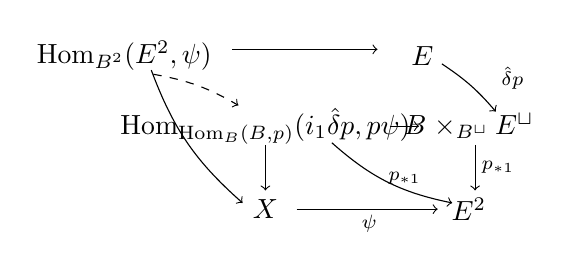
\begin{tikzpicture}[x=1.5em,y=1.5em]
  \node (HB2) at (0,2.4) {$\mathrm{Hom}_{B^{2}}(E^{2},\qcor{\psi})$};
  \node (Esq) at (7.2,2.4) {$E^{\square}$};
  \draw[->] (2.6,2.55) -- (6.1,2.55);
  \node at (4.3,2.85) {$\scriptstyle\llcorner$};
  \draw[->] (7.65,2.2) to[bend left=8] (8.95,1.05);
  \node at (9.35,1.85) {$\scriptstyle\hat{\delta}p$};
  \draw[->,dashed] (0.7,1.95) to[bend left=10] (2.75,1.2);
  \node (HBH) at (3.4,0.7) {$\mathrm{Hom}_{\mathrm{Hom}_{B}(B,p)}(i_{1}\hat{\delta}p,\qcor{p\psi})$};
  \draw[->] (3.4,0.25) -- (3.4,-0.85);
  \node (BB) at (8.3,0.7) {$B^{\square}\times_{B^{\sqcup}}E^{\sqcup}$};
  \draw[->] (6.4,0.7) -- (7.1,0.7);
  \node at (6.85,1.0) {$\scriptstyle\llcorner$};
  \draw[->] (8.45,0.25) -- (8.45,-0.85);
  \node at (9.0,-0.3) {$\scriptstyle p_{*1}$};
  \node (X) at (3.4,-1.3) {$X$};
  \node (E2) at (8.3,-1.3) {$E^{2}$};
  \draw[->] (4.15,-1.3) -- (7.55,-1.3);
  \node at (5.9,-1.65) {$\scriptstyle\qcor{\psi}$};
  \draw[->] (5.0,0.3) to[bend right=15] (7.9,-1.15);
  \node at (6.75,-0.55) {$\scriptstyle p_{*1}$};
  \draw[->] (0.65,2.05) to[bend right=14] (2.85,-1.15);
\end{tikzpicture}
\end{rveq}
由于包含 $\iota$ 可按下左图分解，由附录 C 中的命题 C.2.9(vi)，\trLeibnizCotensor{}%
可按下右图分解：
\begin{center}
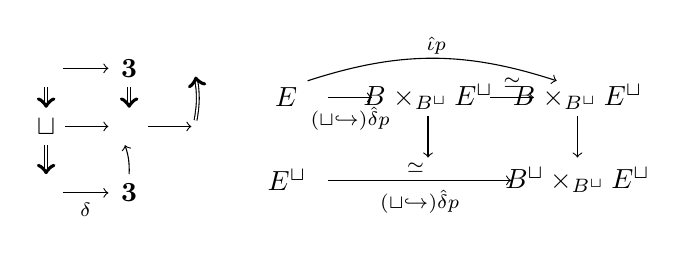
\begin{tikzpicture}[x=1.5em,y=1.5em]
  \node (lc) at (0,1.6) {$\llcorner$};
  \node (t3) at (2.0,1.6) {$\qcThree$};
  \draw[->] (0.4,1.6) -- (1.5,1.6);
  \node (su) at (0,0.2) {$\sqcup$};
  \draw[double,->] (0,1.15) -- (0,0.65);
  \node (bm) at (2.0,0.2) {$\boxminus$};
  \draw[->] (0.45,0.2) -- (1.5,0.2);
  \node at (1.0,0.5) {$\scriptstyle\llcorner$};
  \node (sq) at (4.0,0.2) {$\square$};
  \draw[->] (2.45,0.2) -- (3.5,0.2);
  \node at (3.0,0.5) {$\scriptstyle\llcorner$};
  \draw[double,->] (2.0,1.15) -- (2.0,0.65);
  \draw[double,->] (3.6,0.35) to[bend right=10] (3.6,1.4);
  \node (lc2) at (0,-1.4) {$\llcorner$};
  \draw[double,->] (0,-0.25) -- (0,-0.95);
  \draw[->] (0.4,-1.4) -- node[below]{$\scriptstyle\delta$} (1.5,-1.4);
  \node (t3b) at (2.0,-1.4) {$\qcThree$};
  \draw[->] (2.0,-0.95) to[bend right=10] (1.9,-0.25);
  \node at (4.9,0.1) {$\rightsquigarrow$};
  \begin{scope}[shift={(5.8,0)}]
  \node (Esq) at (0,0.9) {$E^{\square}$};
  \node (Bs1) at (3.4,0.9) {$B^{\square}\times_{B^{\sqcup}}E^{\sqcup}$};
  \node (Bs2) at (7.0,0.9) {$B^{\square}\times_{B^{\sqcup}}E^{\sqcup}$};
  \draw[->] (1.0,0.9) -- node[below]{$\scriptstyle(\sqcup\hookrightarrow\square)\hat{\delta}p$} (2.05,0.9);
  \draw[->] (4.9,0.9) -- node[above]{$\scriptstyle\simeq$} (5.95,0.9);
  \draw[->] (0.5,1.3) to[bend left=18] (6.5,1.3);
  \node at (3.6,2.15) {$\scriptstyle\hat{\iota}p$};
  \draw[->] (3.4,0.45) -- (3.4,-0.55);
  \draw[->] (7.0,0.45) -- (7.0,-0.55);
  \node (Eu) at (0,-1.1) {$E^{\sqcup}$};
  \node (Bu) at (7.0,-1.1) {$B^{\sqcup}\times_{B^{\sqcup}}E^{\sqcup}$};
  \draw[->] (1.0,-1.1) -- node[below]{$\scriptstyle(\sqcup\hookrightarrow\square)\hat{\delta}p$} (5.4,-1.1);
  \node at (3.1,-0.8) {$\scriptstyle\simeq$};
  \end{scope}
\end{tikzpicture}
\end{center}
又由于 $\sqcup\hookrightarrow\square$是某内号角包含的\trPushout，这两支映射中的%
第二支是\trTrivialFibration。由于 $\boxminus\hookrightarrow\square$是 $\delta$
的一个\trPushout，$(\boxminus\hookrightarrow\square)\hat{\delta}p$是%
$\hat{\delta}p$ 的一个\trPullback。由假设 (i)，后一映射沿%
$\qcor{\psi}\colon X\to E^{2}$拉回到一条\trTrivialFibration。于是前一映射亦然，
从而 \eqref{eq:pulled-back-leibniz-square} 中的虚映射是\trTrivialFibration，
这证明了 (ii) 所宣称的绝对提升图。

\textbf{(ii)$\Rightarrow$(iii)：}常值图表函子 $\Delta\colon E\to E^{2}$定义为%
沿函子 $!\colon\qcTwo\to\qcOne$的限制，因而是定义域投影函子 $p_{0}$ 的%
左伴随右逆：
\begin{center}
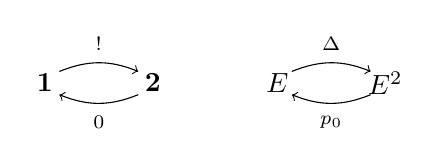
\begin{tikzpicture}[x=1.5em,y=1.5em]
  \node (o1) at (0,0) {$\qcOne$};
  \node (o2) at (2.6,0) {$\qcTwo$};
  \draw[->] (0.35,0.28) to[bend left=22] (2.25,0.28);
  \node at (1.3,0.95) {$\scriptstyle!$};
  \draw[->] (2.25,-0.28) to[bend left=22] (0.35,-0.28);
  \node at (1.3,-0.95) {$\scriptstyle 0$};
  \node at (4.3,0) {$\rightsquigarrow$};
  \begin{scope}[shift={(5.6,0)}]
  \node (E)  at (0,0) {$E$};
  \node (E2) at (2.6,0) {$E^{2}$};
  \draw[->] (0.35,0.28) to[bend left=22] (2.25,0.28);
  \node at (1.3,0.95) {$\scriptstyle\Delta$};
  \draw[->] (2.25,-0.28) to[bend left=22] (0.35,-0.28);
  \node at (1.3,-0.95) {$\scriptstyle p_{0}$};
  \end{scope}
\end{tikzpicture}
\end{center}
特别地，由第 2 章中的引理 2.3.7，\trCounit{} $\nu\colon\Delta p_{0}\Rightarrow\mathrm{id}$
定义了恒同沿 $\Delta$ 的一个绝对右提升。由第 2 章中的引理 2.4.1，这一绝对提升图
与 (ii) 的绝对提升图复合，定义出满足 (iii) 所要求性质的绝对提升图：
\begin{center}
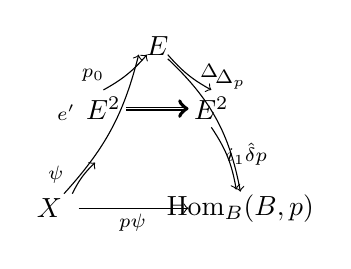
\begin{tikzpicture}[x=1.5em,y=1.5em]
  \node (E)   at (2.6,2.7) {$E$};
  \node (E2a) at (1.3,1.2) {$E^{2}$};
  \node (E2b) at (3.9,1.2) {$E^{2}$};
  \node (X)   at (0,-1.2) {$X$};
  \node (HB)  at (4.6,-1.2) {$\mathrm{Hom}_{B}(B,p)$};
  \draw[->] (0.35,-0.85) to[bend right=14] (2.15,2.5);
  \node at (0.4,1.1) {$\scriptstyle e'$};
  \draw[->] (1.3,1.65) to[bend right=10] (2.35,2.5);
  \node at (1.05,2.0) {$\scriptstyle p_{0}$};
  \draw[->] (2.85,2.5) to[bend right=10] (3.9,1.65);
  \node at (3.85,2.1) {$\scriptstyle\Delta$};
  \draw[double,->] (1.85,1.2) -- (3.35,1.2);
  \draw[->] (0.7,-1.2) -- (3.35,-1.2);
  \node at (2.0,-1.55) {$\scriptstyle\qcor{p\psi}$};
  \draw[->] (0.55,-0.85) to[bend left=10] (1.1,-0.1);
  \node at (0.15,-0.4) {$\scriptstyle\qcor{\psi}$};
  \draw[->] (3.9,0.75) to[bend left=12] (4.5,-0.75);
  \node at (4.75,0.1) {$\scriptstyle i_{1}\hat{\delta}p$};
  \draw[->] (2.85,2.4) to[bend left=18] (4.6,-0.8);
  \node at (4.35,1.9) {$\scriptstyle\Delta_{p}$};
\end{tikzpicture}
\end{center}

\textbf{(iii)$\Rightarrow$(i)：}由定理 3.5.3，一个绝对右提升图表——如 (iii)
所给出的——供应一个\trFiberedEquivalence。对如下左侧的泛型绝对右提升图表，
\trFiberedEquivalence{} $\mathrm{Hom}_{B}(B,r)\simeq_{C\times B}\mathrm{Hom}_{A}(f,g)$
可以通过复合如下右侧图中的诸虚映射来构造——也就是把该映射构造成点线复合映射的%
一个限制（见第 2 章中的引理 2.1.14）：
\begin{center}
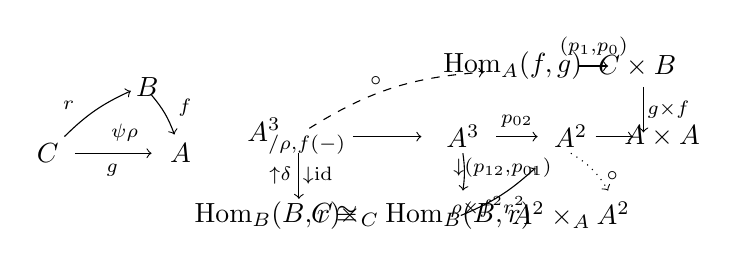
\begin{tikzpicture}[x=1.5em,y=1.5em]
  \node (B) at (2.4,1.6) {$B$};
  \node (C) at (0,0) {$C$};
  \node (A) at (3.2,0) {$A$};
  \draw[->] (0.4,0.4) to[bend left=10] (2.0,1.5);
  \node at (0.5,1.15) {$\scriptstyle r$};
  \draw[->] (2.5,1.4) to[bend left=10] (3.05,0.45);
  \node at (3.3,1.1) {$\scriptstyle f$};
  \draw[->] (0.65,0) -- (2.5,0);
  \node at (1.55,-0.4) {$\scriptstyle g$};
  \node at (1.85,0.5) {$\scriptstyle\psi\rho$};
  \node at (4.6,0.8) {$\rightsquigarrow$};
  \begin{scope}[shift={(5.6,0)}]
  \node (Hfg) at (5.6,2.1) {$\mathrm{Hom}_{A}(f,g)$};
  \node (CB)  at (8.6,2.1) {$C\times B$};
  \draw[->] (7.2,2.1) -- node[above]{$\scriptstyle(p_{1},p_{0})$} (7.9,2.1);
  \node at (7.5,1.75) {$\scriptstyle\llcorner$};
  \draw[->] (8.75,1.6) -- (8.75,0.5);
  \node at (9.35,1.05) {$\scriptstyle g\times f$};
  \draw[->,dashed] (0.7,0.6) to[bend left=14] (4.9,1.95);
  \node at (2.3,1.75) {$\scriptstyle\circ$};
  \node (A3) at (0.4,0.4) {$A^{3}_{/\rho,f(-)}$};
  \draw[->] (1.75,0.4) -- (3.4,0.4);
  \node (A3b) at (4.4,0.4) {$A^{3}$};
  \draw[->] (5.2,0.4) -- node[above]{$\scriptstyle p_{02}$} (6.2,0.4);
  \node (A2) at (7.0,0.4) {$A^{2}$};
  \draw[->] (7.6,0.4) -- (8.5,0.4);
  \node (AA) at (9.2,0.4) {$A\times A$};
  \draw[->] (0.45,0.0) -- (0.45,-1.1);
  \node at (0.0,-0.55) {$\scriptstyle\uparrow\delta$};
  \node at (0.9,-0.55) {$\scriptstyle\downarrow\mathrm{id}$};
  \draw[->] (4.4,0.0) to[bend left=8] (4.4,-0.9);
  \node at (5.35,-0.35) {$\scriptstyle\downarrow(p_{12},p_{01})$};
  \draw[->,dotted] (7.0,0.0) to[bend left=14] (7.9,-0.9);
  \node at (8.0,-0.55) {$\scriptstyle\circ$};
  \node (HB) at (-0.3,-1.5) {$\mathrm{Hom}_{B}(B,r)$};
  \node (iso) at (1.6,-1.5) {$\cong$};
  \node (CH) at (3.4,-1.5) {$C\times_{C}\mathrm{Hom}_{B}(B,r)$};
  \draw[->] (4.35,-1.5) to[bend right=10] (6.15,-0.35);
  \node at (5.0,-1.3) {$\scriptstyle\qcor{\rho}\times f^{2}r^{2}$};
  \node (A22) at (7.0,-1.5) {$A^{2}\times_{A}A^{2}$};
  \end{scope}
\end{tikzpicture}
\end{center}
由\trTwoOfThreeProperty，限制映射
$\circ\colon A^{3}_{/\rho,f(-)}\twoheadrightarrow\mathrm{Hom}_{A}(f,g)$
是一个\trEquivalence。

应用于 (iii) 的绝对右提升图表，这就构造出一条\trTrivialFibration
\begin{rveq}\label{eq:restriction-trivial-fibration}
\mathrm{Hom}_{B}(B,p)^{3}_{(\epsilon,\Delta_{p}(-))}
\xrightarrow[\ ]{\ p_{02}\ }
\mathrm{Hom}_{\mathrm{Hom}_{B}(B,p)}(\Delta_{p},\qcor{p\psi})
\end{rveq}
\eqref{eq:restriction-trivial-fibration} 的定义域是下图表演算出的极限——先拉回%
各行、再对所得\trCospan{}取\trPullback：
\begin{center}
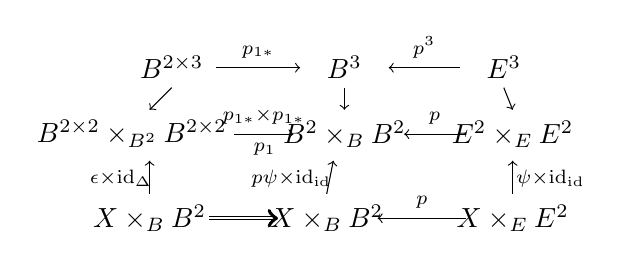
\begin{tikzpicture}[x=1.6em,y=1.6em]
  \node (b23) at (1.5,2.4) {$B^{2\times 3}$};
  \node (b3)  at (5.4,2.4) {$B^{3}$};
  \node (e3)  at (9.0,2.4) {$E^{3}$};
  \draw[->] (2.5,2.4) -- node[above]{$\scriptstyle p_{1*}$} (4.4,2.4);
  \draw[->] (8.0,2.4) -- node[above]{$\scriptstyle p^{3}$} (6.4,2.4);
  \node (b22) at (0.6,0.9) {$B^{2\times 2}\times_{B^{2}}B^{2\times 2}$};
  \node (b22b) at (5.4,0.9) {$B^{2}\times_{B}B^{2}$};
  \node (e22) at (9.2,0.9) {$E^{2}\times_{E}E^{2}$};
  \draw[->] (2.9,0.9) -- node[above]{$\scriptstyle p_{1*}\times p_{1*}$} (4.25,0.9);
  \node at (3.6,0.55) {$\scriptstyle p_{1}$};
  \draw[->] (8.15,0.9) -- node[above]{$\scriptstyle p^{\llcorner}$} (6.75,0.9);
  \node (xb) at (1.0,-1.0) {$X\times_{B}B^{2}$};
  \node (xb2) at (5.0,-1.0) {$X\times_{B}B^{2}$};
  \node (xe)  at (9.2,-1.0) {$X\times_{E}E^{2}$};
  \draw[double,->] (2.35,-1.0) -- (3.9,-1.0);
  \draw[->] (8.15,-1.0) -- node[above]{$\scriptstyle p$} (6.15,-1.0);
  \draw[->] (1.0,-0.45) -- (1.0,0.3);
  \node at (0.35,-0.1) {$\scriptstyle\qcor{\epsilon}\times\mathrm{id}_{\Delta}$};
  \draw[->] (5.0,-0.45) -- (5.15,0.3);
  \node at (4.2,-0.1) {$\scriptstyle\qcor{p\psi}\times\mathrm{id}_{\mathrm{id}}$};
  \draw[->] (9.2,-0.45) -- (9.2,0.3);
  \node at (10.05,-0.1) {$\scriptstyle\qcor{\psi}\times\mathrm{id}_{\mathrm{id}}$};
  \draw[->] (1.5,1.95) -- (1.0,1.45);
  \draw[->] (5.4,1.95) -- (5.4,1.45);
  \draw[->] (9.0,1.95) -- (9.2,1.45);
\end{tikzpicture}
\end{center}
但由超立方体拉回引理，它同样可以取成诸列的\trPullback{}之间诱导出的那个%
\trCospan{}的\trPullback：
\[
\mathrm{Hom}_{B}(B,pe')\times_{B^{2\times\llcorner}}B^{2\times 3}
\xrightarrow{\ p_{1*}\ }\ B_{/p\psi}
\xleftarrow{\ p\ }\ E_{/\psi}
\]
于是我们要寻求对左手列之\trPullback{}的更好理解。

由于 $\epsilon\colon\Delta_{p}e'\Rightarrow\qcor{p\psi}$满足%
$p_{0}\epsilon=\mathrm{id}_{pe'}$，我们可以选取一个表示\trFunctor{}
$\qcor{\epsilon}$，使其穿过如下\trPullback
\begin{center}
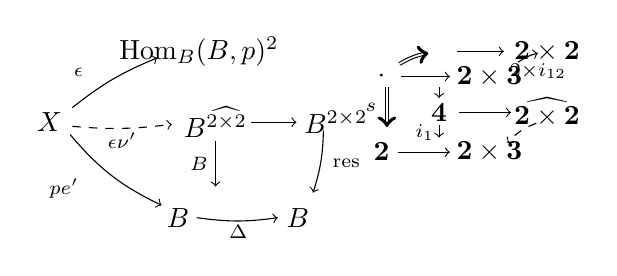
\begin{tikzpicture}[x=1.5em,y=1.5em]
  \node (HB2) at (3.6,2.5) {$\mathrm{Hom}_{B}(B,p)^{2}$};
  \node (X)   at (0,0.8) {$X$};
  \node (Bh)  at (4.0,0.8) {$B^{\widehat{2\times 2}}$};
  \node (B22) at (6.9,0.8) {$B^{2\times 2}$};
  \draw[->] (0.55,1.15) to[bend left=8] (2.6,2.35);
  \node at (0.7,2.0) {$\scriptstyle\qcor{\epsilon}$};
  \draw[->,dashed] (0.55,0.7) to[bend right=6] (2.95,0.75);
  \node at (1.75,0.35) {$\scriptstyle\qcor{\epsilon\nu'}$};
  \draw[->] (4.85,0.8) -- (5.95,0.8);
  \node at (5.35,1.1) {$\scriptstyle\llcorner$};
  \draw[->] (4.0,0.35) -- (4.0,-0.75);
  \node at (3.6,-0.2) {$\scriptstyle B$};
  \draw[->] (0.5,0.5) to[bend right=12] (2.7,-1.2);
  \node at (0.35,-0.8) {$\scriptstyle pe'$};
  \node (B) at (3.1,-1.5) {$B$};
  \draw[->] (3.55,-1.5) to[bend right=8] (5.5,-1.5);
  \node at (4.55,-1.85) {$\scriptstyle\Delta$};
  \node (Bg) at (6.0,-1.5) {$B^{\ulcorner}$};
  \draw[->] (6.6,0.6) to[bend left=8] (6.35,-0.9);
  \node at (7.15,-0.2) {$\scriptstyle\mathrm{res}$};
  \begin{scope}[shift={(8.0,0.6)},x=1.3em,y=1.3em]
  \node (G)  at (1.6,2.2) {$\ulcorner$};
  \node (T22) at (4.6,2.2) {$\qcTwo\times\qcTwo$};
  \draw[->] (2.1,2.2) -- (3.4,2.2);
  \node (qb) at (0,1.5) {$\boxdot\cdot$};
  \node (T23) at (3.0,1.5) {$\qcTwo\times\qcThree$};
  \draw[->,double] (0.5,1.85) to[bend left=10] (1.3,2.15);
  \draw[->] (0.55,1.5) -- (1.9,1.5);
  \draw[->] (3.8,1.9) to[bend left=10] (4.35,2.15);
  \node at (4.35,1.65) {$\scriptstyle 2\times i_{12}$};
  \node (T4) at (1.6,0.5) {$\qcFour$};
  \draw[->] (1.6,1.2) -- (1.6,0.9);
  \draw[->,double] (0.15,1.2) -- (0.15,0.1);
  \node at (-0.3,0.65) {$\scriptstyle s$};
  \node (t2) at (0,-0.6) {$\qcTwo$};
  \draw[->] (1.6,0.15) -- (1.6,-0.2);
  \node at (1.2,-0.05) {$\scriptstyle i_{1}$};
  \node (T2h) at (4.6,0.5) {$\widehat{\qcTwo\times\qcTwo}$};
  \draw[->] (2.15,0.5) -- (3.6,0.5);
  \node at (2.85,0.8) {$\scriptstyle\ulcorner$};
  \draw[->,dashed] (4.3,0.2) to[bend right=14] (3.5,-0.35);
  \node (T23b) at (3.0,-0.6) {$\qcTwo\times\qcThree$};
  \draw[->] (0.45,-0.6) -- (1.9,-0.6);
  \node at (1.15,-0.3) {$\scriptstyle\ulcorner$};
  \end{scope}
\end{tikzpicture}
\end{center}
——它由按立方体后面中单纯集的\trPushout{}所指示的方式，退化 $2\times 2$ 中的始%
\trCospan{}而得。沿 $\Delta\colon B^{2}\to B^{2\times 2}$拉回，则在 $2\times 3$
的左手方块中实现了一种类似的取商，如立方体的前面所示，其中 $s\colon\boxdot\cdot\to\qcTwo$
把左侧两个对象送到 $0$、把右侧三个对象送到 $1$。于是我们看到，映射%
\eqref{eq:restriction-trivial-fibration}定义为沿 $\qcor{\epsilon'}$对下图中的%
映射 $q$ 取\trPullback：
\begin{center}
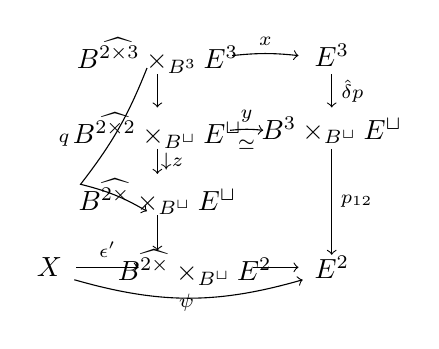
\begin{tikzpicture}[x=1.5em,y=1.5em]
  \node (t1) at (2.6,3.2) {$B^{\widehat{2\times 3}}\times_{B^{3}}E^{3}$};
  \node (E3) at (6.8,3.2) {$E^{3}$};
  \draw[->] (4.4,3.2) to[bend left=6] (6.0,3.2);
  \node at (5.2,3.55) {$\scriptstyle x$};
  \draw[->] (2.6,2.75) -- (2.6,1.95);
  \draw[->] (6.8,2.75) -- (6.8,1.95);
  \node at (7.3,2.35) {$\scriptstyle\hat{\delta}p$};
  \node (m1) at (2.6,1.4) {$B^{\widehat{2\times 2}}\times_{B^{\sqcup}}E^{\sqcup}$};
  \node (m2) at (6.8,1.4) {$B^{3}\times_{B^{\sqcup}}E^{\sqcup}$};
  \draw[->] (4.35,1.4) to[bend left=6] (5.15,1.4);
  \node at (4.75,1.75) {$\scriptstyle y$};
  \node at (4.75,1.05) {$\scriptstyle\simeq$};
  \draw[->] (2.6,0.95) -- (2.6,0.35);
  \node at (2.95,0.65) {$\scriptstyle\downarrow z$};
  \draw[->] (6.8,0.95) -- (6.8,-1.6);
  \node at (7.4,-0.3) {$\scriptstyle p_{12}$};
  \node (l3) at (2.6,-0.2) {$B^{\widehat{2\times\llcorner}}\times_{B^{\sqcup}}E^{\sqcup}$};
  \draw[->] (2.6,-0.65) -- (2.6,-1.5);
  \draw[->] (2.35,2.9) to[bend left=8] (0.75,0.1) to[bend left=8] (2.35,-0.55);
  \node at (0.35,1.15) {$\scriptstyle q$};
  \node (X)  at (0,-1.9) {$X$};
  \node (b2) at (3.5,-1.9) {$B^{\widehat{2\times\llcorner}}\times_{B^{\sqcup}}E^{2}$};
  \node (E2) at (6.8,-1.9) {$E^{2}$};
  \draw[->] (0.65,-1.9) -- node[above]{$\scriptstyle\qcor{\epsilon'}$} (2.15,-1.9);
  \draw[->] (4.9,-1.9) -- (6.0,-1.9);
  \draw[->] (0.6,-2.2) to[bend right=16] (6.1,-2.2);
  \node at (3.3,-2.75) {$\scriptstyle\qcor{\psi}$};
\end{tikzpicture}
\end{center}
我们宣称：被标记为 $x$、$y$ 与 $z$ 的那些映射都是\trTrivialFibration。于是，由%
等价的\trTwoOfThreeProperty{}可得：若 $q$ 沿 $\qcor{\epsilon'}$的\trPullback{}是一个%
\trEquivalence——如 (iii) 的绝对右提升图表所给出的——则 $\hat{\delta}p$ 沿%
$\qcor{\psi}$的\trPullback{}是一个\trEquivalence，这就证明了 (i)。

\trTrivialFibration{} $x$ 与 $y$ 都是限制映射%
$B^{\widehat{2\times 3}}\twoheadrightarrow B^{3}$的\trPullback，我们将证明后者%
是\trTrivialFibration。这是范畴 $\qcThree$、$\boxdot\cdot$、$2\times 3$ 之间的%
一列伴随，它们在商\trSimplicialSet{}之间
\begin{center}
\begin{tikzpicture}[x=1.1em,y=1.1em]
  \node at (0,0) {$\left\{\vcenter{\hbox{\begin{tikzpicture}[x=1.1em,y=1.1em]
    \node at (0,0) {$\scriptstyle 0$};
    \node at (1.6,0) {$\scriptstyle 1$};
    \node at (3.2,0) {$\scriptstyle 2$};
    \draw[->] (0.3,0) -- (1.2,0);
    \draw[->] (1.9,0) -- (2.8,0);
  \end{tikzpicture}}}\right\}$};
  \draw[->] (2.8,0.25) to[bend left=22] (5.4,0.25);
  \draw[->] (5.4,-0.25) to[bend left=22] (2.8,-0.25);
  \node at (4.1,0) {$\scriptstyle\perp$};
  \node at (6.9,0) {$\left\{\vcenter{\hbox{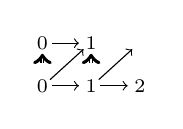
\begin{tikzpicture}[x=1.1em,y=1.1em]
    \node at (0,0.5) {$\scriptstyle 0$};
    \node at (1.6,0.5) {$\scriptstyle 1$};
    \node at (0,-0.9) {$\scriptstyle 0$};
    \node at (1.6,-0.9) {$\scriptstyle 1$};
    \node at (3.2,-0.9) {$\scriptstyle 2$};
    \draw[->] (0.3,0.5) -- (1.2,0.5);
    \draw[double,->] (0,-0.15) -- (0,0.15);
    \draw[double,->] (1.6,-0.15) -- (1.6,0.15);
    \draw[->] (0.3,-0.9) -- (1.2,-0.9);
    \draw[->] (1.9,-0.9) -- (2.8,-0.9);
    \draw[->] (0.25,-0.7) -- (1.35,0.3);
    \draw[->] (1.85,-0.7) -- (2.95,0.3);
  \end{tikzpicture}}}\right\}$};
  \draw[->] (11.6,0.25) to[bend left=22] (14.2,0.25);
  \draw[->] (14.2,-0.25) to[bend left=22] (11.6,-0.25);
  \node at (12.9,0) {$\scriptstyle\perp$};
  \node at (15.9,0) {$\left\{\vcenter{\hbox{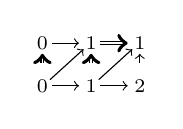
\begin{tikzpicture}[x=1.1em,y=1.1em]
    \node at (0,0.5) {$\scriptstyle 0$};
    \node at (1.6,0.5) {$\scriptstyle 1$};
    \node at (3.2,0.5) {$\scriptstyle 1$};
    \node at (0,-0.9) {$\scriptstyle 0$};
    \node at (1.6,-0.9) {$\scriptstyle 1$};
    \node at (3.2,-0.9) {$\scriptstyle 2$};
    \draw[->] (0.3,0.5) -- (1.2,0.5);
    \draw[double,->] (1.9,0.5) -- (2.8,0.5);
    \draw[double,->] (0,-0.15) -- (0,0.15);
    \draw[double,->] (1.6,-0.15) -- (1.6,0.15);
    \draw[->] (3.2,-0.15) -- (3.2,0.15);
    \draw[->] (0.3,-0.9) -- (1.2,-0.9);
    \draw[->] (1.9,-0.9) -- (2.8,-0.9);
    \draw[->] (0.25,-0.7) -- (1.35,0.3);
    \draw[->] (1.85,-0.7) -- (2.95,0.3);
  \end{tikzpicture}}}\right\}$};
\end{tikzpicture}
\end{center}
成为单纯\trHomotopyEquivalence。
于是，沿该复合包含的限制便定义出一个\trEquivalence{}
$B^{\widehat{2\times 3}}\twoheadrightarrow B^{3}$。映射 $z$ 是%
$B^{\widehat{2\times 3}}\twoheadrightarrow B^{\widehat{2\times\llcorner}}$的一个%
\trPullback，后者是\trTrivialFibration，因为包含%
$2\times\llcorner\hookrightarrow 2\times 3$可以由「特殊外号角」填充（见附录 D
中的定理 D.5.1 与推论 D.3.12）。
这样我们看到，\eqref{eq:restriction-trivial-fibration}与%
\cref{def:pcartesian-arrow}的映射等价，从而 $\psi$ 是 $p$-\trCartesian，
这就证明了 (iii)$\Rightarrow$(i)。
\end{proof}

注意，\eqref{eq:hypercube-weakly-cartesian} 的\trWeaklyCartesianSquare{}底下的%
那个\trCospan{}的数据由一个\trFunctor{} $\qcor{\beta}\colon X\to\mathrm{Hom}_{B}(B,p)$
确定，后者表示一个\trNaturalTransformation{} $\beta\colon b\Rightarrow pe$，
其余定义域沿一个指定的\trFunctor{} $e\colon X\to E$ 穿过 $p$。于是，追问这种%
形式的特定箭头是否具有余定义域为 $e$ 的 $p$-笛卡尔提升，就是切题的。

\begin{definition}[$p$-笛卡尔提升]\label{def:pcartesian-lifts}
设 $p\colon E\twoheadrightarrow B$ 为一条\trIsofibration。称箭头%
$\qcor{\psi}\colon X\to E^{2}$ \textbf{\trLifting}（lift）箭头%
$\qcor{\beta}\colon X\to\mathrm{Hom}_{B}(B,p)$，若左下的三角形交换：
\begin{center}
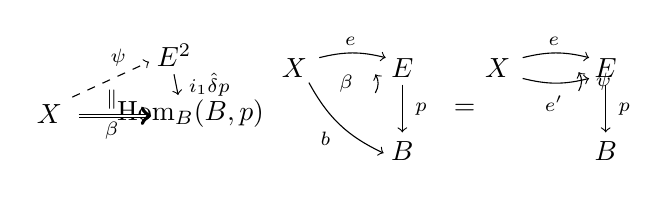
\begin{tikzpicture}[x=1.5em,y=1.5em]
  \node (E2) at (3.0,1.4) {$E^{2}$};
  \node (X)  at (0,0) {$X$};
  \node (HB) at (3.4,0) {$\mathrm{Hom}_{B}(B,p)$};
  \draw[->,dashed] (0.55,0.4) -- node[above,pos=0.6]{$\scriptstyle\qcor{\psi}$} (2.4,1.25);
  \draw[->] (3.0,0.95) -- (3.1,0.45);
  \node at (3.85,0.7) {$\scriptstyle i_{1}\hat{\delta}p$};
  \draw[double,->] (0.7,-0.05) -- (2.45,-0.05);
  \node at (1.5,-0.4) {$\scriptstyle\qcor{\beta}$};
  \node at (1.5,0.35) {$\scriptstyle\parallel$};
  \node at (4.9,0.7) {$\rightsquigarrow$};
  \begin{scope}[shift={(5.9,0)}]
  \node (X) at (0,1.1) {$X$};
  \node (E) at (2.6,1.1) {$E$};
  \node (B) at (2.6,-0.9) {$B$};
  \draw[->] (0.6,1.35) to[bend left=14] (2.2,1.35);
  \node at (1.35,1.75) {$\scriptstyle e$};
  \draw[->] (2.6,0.7) -- (2.6,-0.45);
  \node at (3.05,0.1) {$\scriptstyle p$};
  \draw[->] (0.35,0.75) to[bend right=18] (2.15,-0.95);
  \node at (0.75,-0.6) {$\scriptstyle b$};
  \draw[->] (1.95,0.5) to[bend right=30] (1.95,0.95);
  \node at (1.25,0.72) {$\scriptstyle\beta$};
  \node at (4.1,0.1) {$=$};
  \begin{scope}[shift={(4.9,0)}]
  \node (X) at (0,1.1) {$X$};
  \node (E) at (2.6,1.1) {$E$};
  \node (B) at (2.6,-0.9) {$B$};
  \draw[->] (0.6,1.35) to[bend left=14] (2.2,1.35);
  \node at (1.35,1.75) {$\scriptstyle e$};
  \draw[->] (0.6,0.85) to[bend right=14] (2.2,0.85);
  \node at (1.35,0.25) {$\scriptstyle e'$};
  \draw[->] (1.95,0.55) to[bend right=30] (1.95,1.0);
  \node at (2.55,0.78) {$\scriptstyle\psi$};
  \draw[->] (2.6,0.7) -- (2.6,-0.45);
  \node at (3.05,0.1) {$\scriptstyle p$};
  \end{scope}
  \end{scope}
\end{tikzpicture}
\end{center}
这给出\trHomotopyTwoCategory{}中的粘贴等式 $\beta=p\psi$。\footnote{提升性质
以\trHomotopyTwoCategory{}中的 2-胞腔来陈述，还是以∞-宇宙诸\trFunctorSpace{}%
中的 1-箭头来陈述，并无实质差别：见\cref{ex:homotopy-lifting}。}当%
$\qcor{\psi}$是 $p$-\trCartesian{}时，我们称它定义了 $\qcor{\beta}$ 的一个
\textbf{$p$-笛卡尔提升}（\emph{$p$-cartesian lift}）。
\end{definition}

$p$-笛卡尔变换的\trUniversalProperty{}蕴含：共同的\trNaturalTransformation{}
$\beta\colon b\Rightarrow pe$ 的任意两个 $p$-笛卡尔提升所表示的那些%
\trNaturalTransformation{}是\trFiberedIsomorphism{}的：

\begin{lemma}[笛卡尔提升的唯一性]\label{lem:uniqueness-of-cartesian-lifts}
若\trNaturalTransformation{}
\cellpair{X}{E}{e'}{e}{\psi}
与
\cellpair{X}{E}{e''}{e}{\psi'}
是共同的\trNaturalTransformation{} $\beta\colon b\Rightarrow pe$ 的%
$p$-笛卡尔提升，则存在一个可逆\trNaturalTransformation{}
\cellpair{X}{E}{e''}{e'}{\zeta}
使得 $\psi'=\psi\cdot\zeta$ 且 $p\zeta=\mathrm{id}_{b}$。
\end{lemma}

\begin{proof}
若 $\psi$ 与 $\psi'$ 定义出共同箭头 $\beta$ 的 $p$-笛卡尔提升，则由%
\cref{thm:pcartesian-characterizations}(iii) 我们有 $\qcor{\beta}$沿%
$\Delta_{p}$ 的一对绝对右提升 $(e',\epsilon)$ 与 $(e'',\epsilon')$，满足%
$p_{1}\epsilon=\psi$、$p_{1}\epsilon'=\psi'$，且%
$p_{0}\epsilon=\mathrm{id}_{b}=p_{0}\epsilon'$。由绝对右提升图表的单性，这诱导出%
一个自然同构
\begin{center}
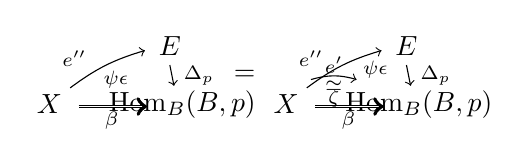
\begin{tikzpicture}[x=1.5em,y=1.5em]
  \node (E)  at (2.9,1.4) {$E$};
  \node (X)  at (0,0) {$X$};
  \node (HB) at (3.2,0) {$\mathrm{Hom}_{B}(B,p)$};
  \draw[->] (0.5,0.4) to[bend left=10] (2.3,1.3);
  \node at (0.6,1.1) {$\scriptstyle e''$};
  \draw[->] (2.9,0.95) -- (3.0,0.45);
  \node at (3.6,0.7) {$\scriptstyle\Delta_{p}$};
  \draw[double,->] (0.7,-0.05) -- (2.35,-0.05);
  \node at (1.5,-0.4) {$\scriptstyle\qcor{\beta}$};
  \node at (1.6,0.6) {$\scriptstyle\psi\epsilon$};
  \node at (4.7,0.7) {$=$};
  \begin{scope}[shift={(5.7,0)}]
  \node (E)  at (2.9,1.4) {$E$};
  \node (X)  at (0,0) {$X$};
  \node (HB) at (3.2,0) {$\mathrm{Hom}_{B}(B,p)$};
  \draw[->] (0.5,0.4) to[bend left=10] (2.3,1.3);
  \node at (0.6,1.1) {$\scriptstyle e''$};
  \draw[->] (2.9,0.95) -- (3.0,0.45);
  \node at (3.6,0.7) {$\scriptstyle\Delta_{p}$};
  \draw[double,->] (0.7,-0.05) -- (2.35,-0.05);
  \node at (1.5,-0.4) {$\scriptstyle\qcor{\beta}$};
  \draw[->] (0.6,0.6) to[bend left=16] (1.7,0.6);
  \node at (1.15,0.95) {$\scriptstyle e'$};
  \node at (1.15,0.15) {$\scriptstyle\zeta$};
  \node at (1.15,0.45) {$\scriptstyle\simeq$};
  \node at (2.15,0.85) {$\scriptstyle\psi\epsilon$};
  \end{scope}
\end{tikzpicture}
\end{center}
使得 $\epsilon'=\epsilon\cdot\Delta_{p}\zeta$。将此等式与 $p_{1}$ 作%
\trWhiskering{}可见 $\psi'=\psi\cdot\zeta$，而与 $p_{0}$ 作\trWhiskering{}可见%
$\mathrm{id}_{b}=p\zeta$。
\end{proof}

把这些结果结合起来，我们得到一个有用的保守性性质：

\begin{lemma}[笛卡尔保守性]\label{lem:cartesian-conservativity}
设有
\cellpair{X}{E}{e'}{e}{\psi}、
\cellpair{X}{E}{e''}{e}{\psi'}
与
\cellpair{X}{E}{e''}{e'}{\zeta}，
它们是\trNaturalTransformation，满足 $\psi$ 与 $\psi'$ 是 $p$-\trCartesian、%
$\psi'=\psi\cdot\zeta$，且 $p\zeta$ 可逆。则 $\zeta$ 可逆。
\end{lemma}

\begin{proof}
由\cref{lem:left-cancellation}与\cref{lem:isomorphism-stability}，$\zeta$ 是某个%
自然同构的 $p$-笛卡尔提升，因而必定可逆。
\end{proof}

刻画 $p$-笛卡尔变换的\cref{thm:pcartesian-characterizations}之\trUniversalProperty{}%
在同伦 2-范畴的层面上产生了归纳与保守性运算，与第 3 章中考虑过的那些运算类似。

\begin{proposition}[$p$-笛卡尔箭头的弱泛性质]\label{prop:pcartesian-weak-universal-property}
设 $p\colon E\twoheadrightarrow B$为\trIsofibration。一支 $p$-笛卡尔箭头
\cellpair{X}{E}{e'}{e}{\psi}
在\trHomotopyTwoCategory{}中具有由以下两种运算给出的弱\trUniversalProperty：
\begin{enumerate}[label=(\roman*)]
\item \textbf{归纳：}给定任意 2-胞腔
\cellpair{X}{E}{e''}{e}{\tau}
与
\cellpair{X}{B}{pe''}{pe'}{\gamma}，
使得 $p\tau=p\psi\cdot\gamma$，则存在 $\gamma$ 的一个\trLifting{}
\cellpair{X}{E}{e''}{e'}{\bar{\gamma}}
使得 $\tau=\psi\cdot\bar{\gamma}$：
\begin{center}
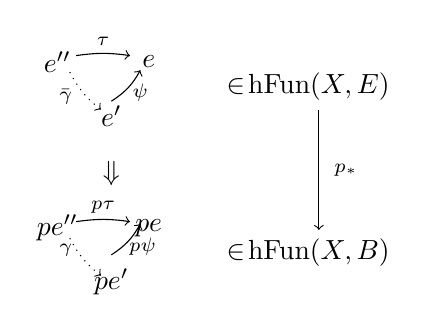
\begin{tikzpicture}[x=1.5em,y=1.5em]
  \node (e2) at (0,1.3) {$e''$};
  \node (e)  at (2.2,1.3) {$e$};
  \draw[->] (0.45,1.45) to[bend left=8] (1.75,1.45);
  \node at (1.1,1.8) {$\scriptstyle\tau$};
  \draw[->,dotted] (0.3,1.05) to[bend right=12] (1.05,0.15);
  \node at (0.2,0.45) {$\scriptstyle\bar{\gamma}$};
  \draw[->] (1.3,0.35) to[bend right=14] (2.0,1.1);
  \node at (2.0,0.55) {$\scriptstyle\psi$};
  \node (ep) at (1.3,0.0) {$e'$};
  \node at (4.3,0.7) {$\in$};
  \node at (6.3,0.7) {$\mathrm{hFun}(X,E)$};
  \node at (1.3,-1.4) {$\Downarrow$};
  \node (pe2) at (0,-2.7) {$pe''$};
  \node (pe)  at (2.2,-2.7) {$pe$};
  \draw[->] (0.45,-2.55) to[bend left=8] (1.75,-2.55);
  \node at (1.1,-2.2) {$\scriptstyle p\tau$};
  \draw[->,dotted] (0.3,-2.95) to[bend right=12] (1.05,-3.85);
  \node at (0.2,-3.25) {$\scriptstyle\gamma$};
  \draw[->] (1.3,-3.35) to[bend right=14] (2.0,-2.6);
  \node at (2.05,-3.15) {$\scriptstyle p\psi$};
  \node (pep) at (1.3,-4.0) {$pe'$};
  \node at (4.3,-3.3) {$\in$};
  \node at (6.3,-3.3) {$\mathrm{hFun}(X,B)$};
  \draw[->] (6.3,0.15) -- (6.3,-2.75);
  \node at (6.95,-1.3) {$\scriptstyle p_{*}$};
\end{tikzpicture}
\end{center}
\item \textbf{保守性：}$\psi$ 的任何纤维化自同态皆可逆：若%
$\zeta\colon e'\Rightarrow e'$是任一满足 $\psi\cdot\zeta=\psi$ 且%
$p\zeta=\mathrm{id}_{pe'}$的\trNaturalTransformation，则 $\zeta$ 可逆。
\end{enumerate}
\end{proposition}

\begin{proof}
保守性性质 (ii) 是\cref{lem:cartesian-conservativity}中观察到的保守性结果的
一个特例，故只需证 (i)。

偶对 $\tau\colon e''\Rightarrow e$ 与 $\gamma\colon pe''\Rightarrow pe'$
满足第 3 章中的命题 3.4.6 所要求的相容性条件，从而诱导出如下左侧的%
\trNaturalTransformation{} $\sigma$，满足 $p_{1}\sigma=\tau$ 与%
$p_{0}\sigma=\gamma$。由于 $\psi$ 是 $p$-\trCartesian，此 2-胞腔穿过%
\cref{thm:pcartesian-characterizations}(iii) 的绝对右提升图表分解：
\begin{center}
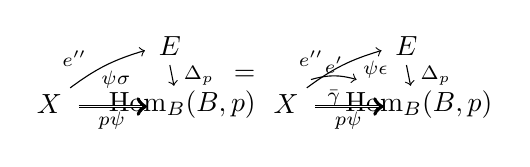
\begin{tikzpicture}[x=1.5em,y=1.5em]
  \node (E)  at (2.9,1.4) {$E$};
  \node (X)  at (0,0) {$X$};
  \node (HB) at (3.2,0) {$\mathrm{Hom}_{B}(B,p)$};
  \draw[->] (0.5,0.4) to[bend left=10] (2.3,1.3);
  \node at (0.6,1.1) {$\scriptstyle e''$};
  \draw[->] (2.9,0.95) -- (3.0,0.45);
  \node at (3.6,0.7) {$\scriptstyle\Delta_{p}$};
  \draw[double,->] (0.7,-0.05) -- (2.35,-0.05);
  \node at (1.5,-0.4) {$\scriptstyle\qcor{p\psi}$};
  \node at (1.6,0.6) {$\scriptstyle\psi\sigma$};
  \node at (4.7,0.7) {$=$};
  \begin{scope}[shift={(5.7,0)}]
  \node (E)  at (2.9,1.4) {$E$};
  \node (X)  at (0,0) {$X$};
  \node (HB) at (3.2,0) {$\mathrm{Hom}_{B}(B,p)$};
  \draw[->] (0.5,0.4) to[bend left=10] (2.3,1.3);
  \node at (0.6,1.1) {$\scriptstyle e''$};
  \draw[->] (2.9,0.95) -- (3.0,0.45);
  \node at (3.6,0.7) {$\scriptstyle\Delta_{p}$};
  \draw[double,->] (0.7,-0.05) -- (2.35,-0.05);
  \node at (1.5,-0.4) {$\scriptstyle\qcor{p\psi}$};
  \draw[->] (0.6,0.6) to[bend left=16] (1.7,0.6);
  \node at (1.15,0.95) {$\scriptstyle e'$};
  \node at (1.15,0.15) {$\scriptstyle\bar{\gamma}$};
  \node at (2.15,0.85) {$\scriptstyle\psi\epsilon$};
  \end{scope}
\end{tikzpicture}
\end{center}
由于 $(e',\epsilon)$ 是绝对右提升，$(e'',\sigma)$ 诱导出一个%
\trNaturalTransformation{} $\bar{\gamma}\colon e''\Rightarrow e'$，使得%
$\sigma=\epsilon\cdot\Delta_{p}\bar{\gamma}$。将这些等式与 $p_{1}$ 作%
\trWhiskering{}可见 $\tau=\psi\cdot\bar{\gamma}$，而与 $p_{0}$ 作%
\trWhiskering{}可见 $\gamma=p\bar{\gamma}$。
\end{proof}

\cref{prop:pcartesian-weak-universal-property}所列举的诸\trUniversalProperty{}%
远弱于\cref{def:pcartesian-arrow}所表达的那一个。的确，它们既不表达%
\cref{lem:cartesian-conservativity}中观察到的完整保守性，也没有利用笛卡尔变换与
绝对右提升图表的限制稳定性。尽管如此，在 $p$ 是\trCartesianFibration{}的条件下，
条件 (i) 与 (ii) 已足以刻画 $p$-笛卡尔变换类——\trCartesianFibration{}这一概念
将在下一节引入。更出人意料的是，若以一条限制稳定性性质增强 (i) 与 (ii)，命题
5.2.11 表明，完全可以仅从\trHomotopyTwoCategory{}的视角定义%
\trCartesianFibration，而无需援引\cref{def:pcartesian-arrow}。然而，即便在%
$p$ 本身并非\trCartesianFibration{}的情形下（例如见%
\cref{ex:codomain-projection-cartesian-arrows}），$p$-笛卡尔箭头也自有其独立的
研究价值；此时我们把笛卡尔纤维化理论的纯 2-范畴式发展置于次要地位，转而请读者
查阅 [110]。


\subsection*{练习}

\begin{exercise}\label{ex:homotopy-lifting}
回忆：\trInfinityCosmos{}中的诸箭头 $\qcor{\psi}\colon X\to E^{2}$对应于\trFunctorSpace{}
$\mathrm{Fun}(X,E)$ 中的一些 1-\trSimplex{}（亦即 1-箭头）$\psi\colon e'\to e$，
而一平行 1-箭头对表示同一个 2-胞腔
\cellpair{X}{E}{e'}{e}{\psi}
当且仅当二者\trHomotopic——即在 $\mathrm{Fun}(X,E)$ 中围出一条 2-箭头，
其第 0 条或第 2 条棱是退化的（见练习 3.2.i）。
证明：若 $p\colon E\twoheadrightarrow B$是一条\trIsofibration，使得每个%
\trNaturalTransformation{} $\beta\colon b\Rightarrow pe$ 在%
\trHomotopyTwoCategory{}中都容有一个\trLifting{} $\psi\colon e'\Rightarrow e$，
则 $\mathrm{Fun}(X,B)$ 中的每支 1-箭头 $\qcor{\beta}\colon b\to pe$ 都按%
\cref{def:pcartesian-lifts}的意义容有一个 1-箭头\trLifting{} $\psi\colon e'\to e$。
\end{exercise}

\begin{exercise}\label{ex:codomain-projection-cartesian-arrows}
（5.2.10）
\begin{enumerate}[label=(\roman*)]
\item 刻画余定义域投影函子 $p_{1}\colon A^{2}\twoheadrightarrow A$的%
\trCartesianArrow。
\item 用 (i) 的答案给出第 4 章中的命题 4.3.11 的另一个证明。
\end{enumerate}
\end{exercise}
   %
\providecommand{\qcor}[1]{\ulcorner#1\urcorner}   %
\providecommand{\qcTwo}{\mathbf{2}}   %
\providecommand{\qcThree}{\mathbf{3}} %
\providecommand{\cellpair}[5]{$\vcenter{\hbox{\begin{tikzpicture}[x=1.15em,y=1.15em]%
\node (s) at (0,0) {$#1$};%
\node (t) at (4.2,0) {$#2$};%
\draw[->] (0.75,0.32) to[bend left=18] (3.45,0.32);%
\node at (2.1,0.88) {$\scriptstyle#3$};%
\draw[->] (0.75,-0.32) to[bend right=18] (3.45,-0.32);%
\node at (2.1,-0.93) {$\scriptstyle#4$};%
\draw[->] (1.95,0.2) to[bend right=32] (1.95,-0.2);%
\node at (2.85,0) {$\scriptstyle#5$};%
\end{tikzpicture}}}$\ignorespaces}

\section{笛卡尔纤维化}\label{sec:cartesian-fibrations}

\trInfinityCategory{}之间的\emph{Grothendieck \trFibration}（Grothendieck fibration）
推广了普通 1-范畴之间的 Grothendieck \trFibration。这一概念由%
Joyal [62] 与 Lurie [78] 首先推广到\trQuasiCategory，又由 Boavida de Brito [34]
与 Rasekh [98, 97] 推广到\trCompleteSegalSpaces。(∞,1)-范畴之间的%
\trCartesianFibration{}已被 Mazel-Gee [86] 与 Ayala–Francis [5] 以模型无关的方式
研究过。

\begin{definition}[笛卡尔纤维化]\label{def:cartesian-fibration}
设 $p\colon E\twoheadrightarrow B$ 为一条\trIsofibration。若任何形如下中图的%
\trNaturalTransformation{} $\beta\colon b\Rightarrow pe$ 都容有一个如下右图的%
$p$-笛卡尔提升 $\chi_{\beta}\colon\beta^{*}e\Rightarrow e$，则 $p$ 是一条%
\trCartesianFibration：
\begin{center}
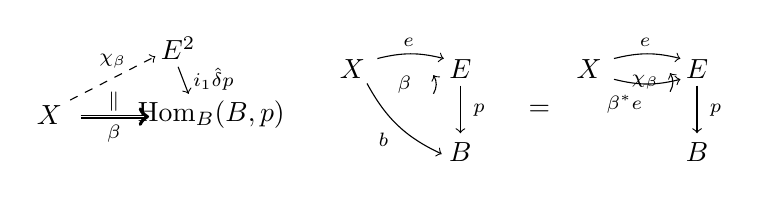
\begin{tikzpicture}[x=1.5em,y=1.5em]
  \node (E2) at (3.1,1.6) {$E^{2}$};
  \node (X)  at (0,0) {$X$};
  \node (HB) at (3.9,0) {$\mathrm{Hom}_{B}(B,p)$};
  \draw[->,dashed] (0.5,0.35) -- node[above,pos=0.5]{$\scriptstyle\qcor{\chi_{\beta}}$} (2.55,1.4);
  \draw[->] (3.1,1.15) -- (3.35,0.5);
  \node at (3.95,0.85) {$\scriptstyle i_{1}\hat{\delta}p$};
  \draw[double,->] (0.75,-0.05) -- (2.4,-0.05);
  \node at (1.55,0.32) {$\scriptstyle\parallel$};
  \node at (1.55,-0.45) {$\scriptstyle\qcor{\beta}$};
  \node at (6.1,0.7) {$\rightsquigarrow$};
  \begin{scope}[shift={(7.3,0)}]
  \node (E) at (2.6,1.1) {$E$};
  \node (X) at (0,1.1) {$X$};
  \node (B) at (2.6,-0.9) {$B$};
  \draw[->] (0.6,1.35) to[bend left=14] (2.2,1.35);
  \node at (1.35,1.75) {$\scriptstyle e$};
  \draw[->] (2.6,0.7) -- (2.6,-0.45);
  \node at (3.05,0.1) {$\scriptstyle p$};
  \draw[->] (0.35,0.75) to[bend right=18] (2.15,-0.95);
  \node at (0.75,-0.6) {$\scriptstyle b$};
  \draw[->] (1.95,0.5) to[bend right=30] (1.95,0.95);
  \node at (1.25,0.72) {$\scriptstyle\beta$};
  \node at (4.5,0.1) {$=$};
  \end{scope}
  \begin{scope}[shift={(13.0,0)}]
  \node (E) at (2.6,1.1) {$E$};
  \node (X) at (0,1.1) {$X$};
  \node (B) at (2.6,-0.9) {$B$};
  \draw[->] (0.6,1.35) to[bend left=14] (2.2,1.35);
  \node at (1.35,1.75) {$\scriptstyle e$};
  \draw[->] (0.6,0.85) to[bend right=14] (2.2,0.85);
  \node at (0.85,0.25) {$\scriptstyle\beta^{*}e$};
  \draw[->] (2.6,0.7) -- (2.6,-0.45);
  \node at (3.05,0.1) {$\scriptstyle p$};
  \draw[->] (1.95,0.55) to[bend right=30] (1.95,1.0);
  \node at (1.35,0.78) {$\scriptstyle\chi_{\beta}$};
  \end{scope}
\end{tikzpicture}
\end{center}
\end{definition}

由练习 5.1.i，提升性质究竟像上右图那样在\trHomotopyTwoCategory{}中表述，还是像
上左图那样用表示箭头来表述，并没有任何差别。

\begin{remark}\label{rem:equivalence-invariance}
\trInfinityCategory{}论的一条指导性原则是：一切\trInfinityCategory{}概念都应当
是\trEquivalence{}不变的。然而，若把 $E$ 与 $B$ 换成与之等价的%
\trInfinityCategory{} $E'$ 与 $B'$，那个与原来等价的函子 $p'\colon E\to B$
却未必是\trIsofibration。不过，由
引理 1.2.19，$p'$ 在 $B'$ 之上等价于某条\trIsofibration{} $p''$，因此我们本可以
在 $p''$ 是\cref{def:cartesian-fibration}意义下的\trIsofibration{}时，就宣布
$p'$ 为\trCartesianFibration。由推论 5.3.1，这一定义至此便是\trEquivalence{}不
变的。出于诸如命题 6.3.14 之类的技术性原因，我们更愿意让%
\cref{def:cartesian-fibration}保持其原貌。
\end{remark}

\trCartesianFibration{}的某些稳定性性质可以直接从这个定义出发来证明。

\begin{lemma}\label{lem:composite-cartesian-fibration}
若 $p\colon E\twoheadrightarrow B$ 与 $q\colon B\twoheadrightarrow A$ 都是%
\trCartesianFibration，则 $qp\colon E\twoheadrightarrow A$ 亦然。此外，%
\trNaturalTransformation
\cellpair{X}{E}{e'}{e}{\psi}
是 $qp$-\trCartesian，当且仅当 $\psi$ 是 $p$-\trCartesian{}且 $p\psi$ 是
$q$-\trCartesian。
\end{lemma}

\begin{proof}
第一条论断立即可由第二条推出：所需的提升可以先取一条 $q$-笛卡尔提升%
$\chi_{\alpha}$、再对该提升后的胞腔取 $p$-笛卡尔提升 $\chi_{\chi_{\alpha}}$ 而
构造出来。
\begin{center}
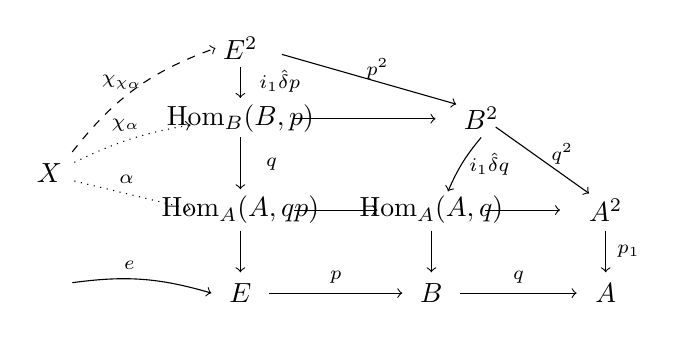
\begin{tikzpicture}[x=1.5em,y=1.5em]
  \node (E2)  at (4.6,4.3) {$E^{2}$};
  \node (HB)  at (4.6,2.6) {$\mathrm{Hom}_{B}(B,p)$};
  \node (B2)  at (10.4,2.6) {$B^{2}$};
  \node (X)   at (0,1.3) {$X$};
  \node (HA)  at (4.6,0.4) {$\mathrm{Hom}_{A}(A,qp)$};
  \node (HAq) at (9.2,0.4) {$\mathrm{Hom}_{A}(A,q)$};
  \node (A2)  at (13.4,0.4) {$A^{2}$};
  \node (E)   at (4.6,-1.6) {$E$};
  \node (B)   at (9.2,-1.6) {$B$};
  \node (A)   at (13.4,-1.6) {$A$};
  \draw[->,dashed] (0.55,1.8) to[bend left=16] node[above,pos=0.4]{$\scriptstyle\qcor{\chi_{\chi_{\alpha}}}$} (4.0,4.3);
  \draw[->] (4.6,3.85) -- (4.6,3.1);
  \node at (5.55,3.5) {$\scriptstyle i_{1}\hat{\delta}p$};
  \draw[->] (5.6,4.15) -- (9.8,2.95);
  \node at (7.9,3.8) {$\scriptstyle p^{2}$};
  \draw[->] (5.9,2.6) -- (9.3,2.6);
  \node at (6.4,2.9) {$\scriptstyle\llcorner$};
  \draw[->] (4.6,2.15) -- (4.6,0.9);
  \node at (5.35,1.5) {$\scriptstyle q$};
  \draw[->] (10.4,2.15) to[bend right=8] (9.6,0.85);
  \node at (10.6,1.5) {$\scriptstyle i_{1}\hat{\delta}q$};
  \draw[->] (10.75,2.4) -- (13.0,0.8);
  \node at (12.35,1.75) {$\scriptstyle q^{2}$};
  \draw[->,dotted] (0.6,1.55) to[bend left=8] node[above,pos=0.45]{$\scriptstyle\qcor{\chi_{\alpha}}$} (3.4,2.45);
  \draw[->,dotted] (0.6,1.1) -- node[above,pos=0.45]{$\scriptstyle\qcor{\alpha}$} (3.4,0.42);
  \draw[->] (5.9,0.4) -- (7.9,0.4);
  \node at (6.35,0.05) {$\scriptstyle\llcorner$};
  \draw[->] (10.5,0.4) -- (12.3,0.4);
  \node at (10.95,0.05) {$\scriptstyle\llcorner$};
  \draw[->] (13.4,-0.1) -- (13.4,-1.1);
  \node at (13.95,-0.6) {$\scriptstyle p_{1}$};
  \draw[->] (4.6,-0.1) -- (4.6,-1.1);
  \draw[->] (9.2,-0.1) -- (9.2,-1.1);
  \draw[->] (0.55,-1.35) to[bend left=12] node[above,pos=0.4]{$\scriptstyle e$} (3.9,-1.6);
  \draw[->] (5.3,-1.6) -- node[above]{$\scriptstyle p$} (8.5,-1.6);
  \draw[->] (9.9,-1.6) -- node[above]{$\scriptstyle q$} (12.7,-1.6);
\end{tikzpicture}
\end{center}
为证明第二条论断，先考虑一支\trNaturalTransformation{}
$\psi\colon e'\Rightarrow e$：设其为 $p$-\trCartesian，且 $p\psi$ 为
$q$-\trCartesian。由引理 5.1.2，这些性质由诸虚\trTrivialFibration{}%
表达，其中后者经拉回可定义出点线\trTrivialFibration：
\begin{center}
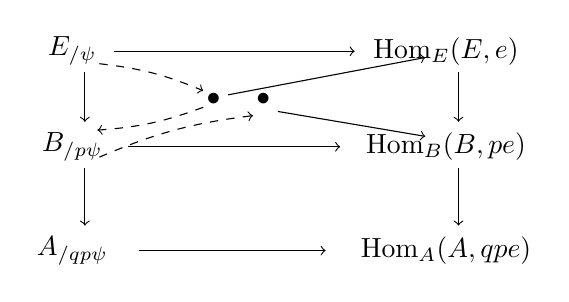
\begin{tikzpicture}[x=1.5em,y=1.5em]
  \node (Ep) at (0,4.4) {$E_{/\psi}$};
  \node (HE) at (9.0,4.4) {$\mathrm{Hom}_{E}(E,e)$};
  \node (Bp) at (0,2.1) {$B_{/p\psi}$};
  \node (HB) at (9.0,2.1) {$\mathrm{Hom}_{B}(B,pe)$};
  \node (Ap) at (0,-0.4) {$A_{/qp\psi}$};
  \node (HA) at (9.0,-0.4) {$\mathrm{Hom}_{A}(A,qpe)$};
  \draw[->] (1.0,4.4) -- (6.8,4.4);
  \draw[->] (1.35,2.1) -- (6.45,2.1);
  \draw[->] (1.6,-0.4) -- (6.1,-0.4);
  \draw[->] (0.3,3.9) -- (0.3,2.7);
  \draw[->] (9.3,3.9) -- (9.3,2.7);
  \draw[->] (0.3,1.6) -- (0.3,0.2);
  \draw[->] (9.3,1.6) -- (9.3,0.2);
  \node at (3.4,3.25) {$\bullet$};
  \node at (3.85,2.95) {$\scriptstyle\lrcorner$};
  \draw[->,dashed] (0.65,4.1) to[bend left=8] (3.15,3.45);
  \draw[->,dashed] (3.15,3.05) to[bend left=8] (0.6,2.5);
  \draw[->] (3.75,3.35) -- (8.5,4.25);
  \node at (4.6,3.25) {$\bullet$};
  \node at (5.05,2.95) {$\scriptstyle\lrcorner$};
  \draw[->,dashed] (0.65,1.85) to[bend left=8] (4.35,2.85);
  \draw[->] (4.95,2.95) -- (8.5,2.35);
\end{tikzpicture}
\end{center}
由于\trTrivialFibration{}可复合，这告诉我们
$E_{/\psi}\twoheadrightarrow A_{/qp\psi}\times_{\mathrm{Hom}_{A}(A,qpe)}\mathrm{Hom}_{E}(E,e)$
是一条\trTrivialFibration，从而 $\psi$ 是 $qp$-\trCartesian。

反之，若 $\psi$ 是 $qp$-\trCartesian，则由引理 5.1.11，它与 $qp\psi$ 的所有其余%
$qp$-笛卡尔提升同构。上面给出的构造对任何一支 $p$-笛卡尔、且在 $p$ 之下的像为%
$q$-\trCartesian 2-胞腔都产生一个 $qp$-笛卡尔提升。由引理 5.1.6 关于 $p$-与%
$q$-笛卡尔变换的同构稳定性，$\psi$ 也必具备这些性质。
\end{proof}

\begin{proposition}[拉回稳定性]\label{prop:pullback-stability}
在任何\trPullback{}方块
\begin{center}
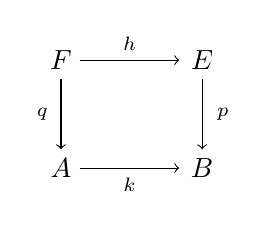
\begin{tikzpicture}[x=1.5em,y=1.5em]
  \node (F) at (0,1.3) {$F$};
  \node (E) at (3.4,1.3) {$E$};
  \node (A) at (0,-1.3) {$A$};
  \node (B) at (3.4,-1.3) {$B$};
  \draw[->] (0.45,1.3) -- node[above]{$\scriptstyle h$} (2.85,1.3);
  \draw[->] (0.45,-1.3) -- node[below]{$\scriptstyle k$} (2.85,-1.3);
  \draw[->] (0,0.85) -- (0,-0.85);
  \node at (-0.45,0) {$\scriptstyle q$};
  \draw[->] (3.4,0.85) -- (3.4,-0.85);
  \node at (3.9,0) {$\scriptstyle p$};
  \node at (0.45,0.85) {$\scriptstyle\llcorner$};
\end{tikzpicture}
\end{center}
中，若 $p$ 是一条\trCartesianFibration，则 $q$ 亦是。此外，余定义域为 $F$ 的%
\trNaturalTransformation{} $\psi$ 是 $q$-\trCartesian，当且仅当 $h\psi$ 是%
$p$-\trCartesian。
\end{proposition}

\begin{proof}
题设中的\trPullback{}方块诱导出 $i_{1}\colon 1\hookrightarrow 2$ 分别与 $q$ 和
$p$ 的\trLeibnizCotensor{}之间的一个\trPullback{}方块。考虑表示\trNaturalTransformation{}
$\alpha\colon a\Rightarrow qf$ 的一支箭头 $\qcor{\alpha}\colon X\to\mathrm{Hom}_{A}(A,q)$。
由于 $p$ 是\trCartesianFibration，\trNaturalTransformation{}
$k\alpha\colon ka\Rightarrow kqf=phf$ 容有一个 $p$-笛卡尔提升 $\qcor{\tau}$，
后者借助\trPullback{}的\trUniversalProperty{}诱导出一个提升
$\qcor{\sigma}\colon X\to F^{2}$，满足 $\qcor{h\sigma}$ 是 $p$-笛卡尔箭头：
\begin{center}
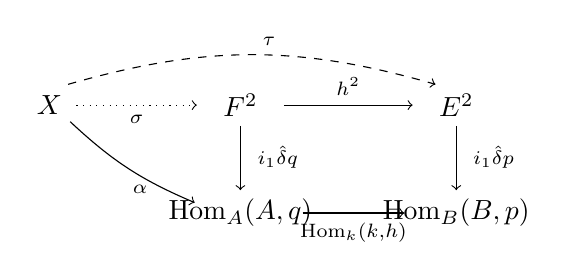
\begin{tikzpicture}[x=1.5em,y=1.5em]
  \node (X)  at (0,1.3) {$X$};
  \node (F2) at (4.6,1.3) {$F^{2}$};
  \node (E2) at (9.8,1.3) {$E^{2}$};
  \node (HA) at (4.6,-1.3) {$\mathrm{Hom}_{A}(A,q)$};
  \node (HB) at (9.8,-1.3) {$\mathrm{Hom}_{B}(B,p)$};
  \draw[->,dotted] (0.65,1.3) -- node[below]{$\scriptstyle\qcor{\sigma}$} (3.55,1.3);
  \draw[->] (5.65,1.3) -- node[above]{$\scriptstyle h^{2}$} (8.75,1.3);
  \node at (5.1,0.95) {$\scriptstyle\llcorner$};
  \draw[->] (0.5,0.9) to[bend right=10] node[below,pos=0.6]{$\scriptstyle\qcor{\alpha}$} (3.5,-1.05);
  \draw[->] (4.6,0.8) -- (4.6,-0.75);
  \node at (5.5,0.05) {$\scriptstyle i_{1}\hat{\delta}q$};
  \draw[->] (9.8,0.8) -- (9.8,-0.75);
  \node at (10.7,0.05) {$\scriptstyle i_{1}\hat{\delta}p$};
  \draw[->] (6.1,-1.3) -- node[below]{$\scriptstyle\mathrm{Hom}_{k}(k,h)$} (8.55,-1.3);
  \draw[->,dashed] (0.45,1.8) to[bend left=16] node[above,pos=0.55]{$\scriptstyle\qcor{\tau}$} (9.3,1.8);
\end{tikzpicture}
\end{center}

所以，如果我们证明了题设的第二部分——余定义域为 $F$ 的\trNaturalTransformation{}
$\psi\colon f'\Rightarrow f$ 是 $q$-\trCartesian，当且仅当 $h\psi$ 是 $p$-\trCartesian
——那么我们就证明了 $q$ 本身是一条\trCartesianFibration，其笛卡尔胞腔由%
\trPullback{}创造。

为此目的，考虑如下立方体：
\begin{center}
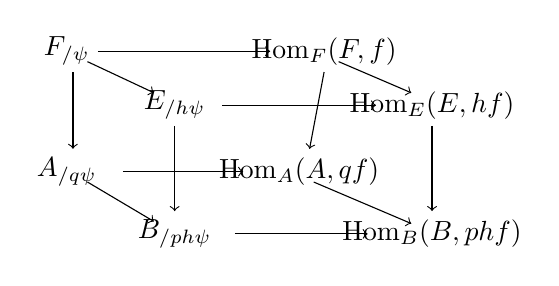
\begin{tikzpicture}[x=1.5em,y=1.5em]
  \node (Fp)  at (0,3.4) {$F_{/\psi}$};
  \node (HFf) at (6.2,3.4) {$\mathrm{Hom}_{F}(F,f)$};
  \node (Eh)  at (2.6,2.1) {$E_{/h\psi}$};
  \node (HEh) at (8.8,2.1) {$\mathrm{Hom}_{E}(E,hf)$};
  \node (Aq)  at (0,0.5) {$A_{/q\psi}$};
  \node (HAq) at (5.6,0.5) {$\mathrm{Hom}_{A}(A,qf)$};
  \node (Bph) at (2.6,-1.0) {$B_{/ph\psi}$};
  \node (HBp) at (8.8,-1.0) {$\mathrm{Hom}_{B}(B,phf)$};
  \draw[->] (0.75,3.4) -- (4.9,3.4);
  \draw[->] (3.75,2.1) -- (7.45,2.1);
  \draw[->] (1.35,0.5) -- (4.25,0.5);
  \draw[->] (4.05,-1.0) -- (7.25,-1.0);
  \draw[->] (0.15,2.9) -- (0.15,1.05);
  \draw[->] (2.6,1.6) -- (2.6,-0.45);
  \draw[->] (6.2,2.9) -- (5.85,1.05);
  \draw[->] (8.8,1.6) -- (8.8,-0.45);
  \draw[->] (0.5,3.15) -- (2.1,2.4);
  \node at (0.55,2.7) {$\scriptstyle\llcorner$};
  \draw[->] (6.55,3.15) -- (8.3,2.4);
  \draw[->] (0.5,0.25) -- (2.1,-0.7);
  \node at (0.55,-0.15) {$\scriptstyle\llcorner$};
  \draw[->] (5.95,0.25) -- (8.3,-0.75);
\end{tikzpicture}
\end{center}
由超立方体拉回引理，左面与右面都是严格的\trPullback{}方块。于是，从
$E_{/h\psi}$ 到前面中\trPullback{}的映射经拉回即得从 $F_{/\psi}$ 到后面中%
\trPullback{}的映射。从而，由命题 3.3.4，若 $h\psi$ 是 $p$-\trCartesian，则 $\psi$
是 $q$-\trCartesian。这就完成了 $q$ 是\trCartesianFibration{}的证明。

现在，若 $\psi$ 是 $q$-\trCartesian，则由引理 5.1.11，$\psi$ 与本证明第一部分中
构造的 $q\psi$ 的 $q$-笛卡尔提升 $\sigma$ 同构。于是 $h\psi$ 与 $h\sigma=\tau$
同构，后者是 $p$-\trCartesian，故由引理 5.1.6，$h\psi$ 也必是 $p$-\trCartesian。
\end{proof}

事实上，在\cref{def:cartesian-fibration}中只需假设：余定义域穿过 $p$ 的那个
泛变换容有一个 $p$-笛卡尔提升：

\begin{lemma}\label{lem:right-comma-cone-lift}
一条\trIsofibration{} $p\colon E\twoheadrightarrow B$ 是\trCartesianFibration，
当且仅当下方左图展示的 $p$ 之上的右逗号锥容有一个如下右图所示的 $p$-笛卡尔提升
$\chi$：
\begin{rveq}\label{eq:right-comma-cone}
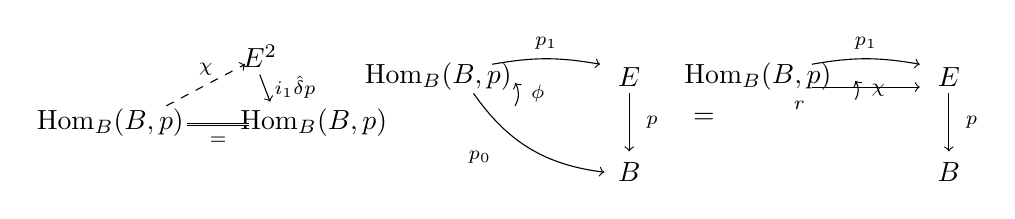
\begin{tikzpicture}[x=1.5em,y=1.5em]
  \node (E2) at (3.6,1.6) {$E^{2}$};
  \node (H1) at (0,0) {$\mathrm{Hom}_{B}(B,p)$};
  \node (H2) at (4.9,0) {$\mathrm{Hom}_{B}(B,p)$};
  \draw[->,dashed] (1.35,0.4) -- node[above,pos=0.5]{$\scriptstyle\qcor{\chi}$} (3.25,1.4);
  \draw[->] (3.6,1.15) -- (3.85,0.5);
  \node at (4.45,0.85) {$\scriptstyle i_{1}\hat{\delta}p$};
  \draw[double] (1.85,-0.05) -- (3.35,-0.05);
  \node at (2.6,-0.45) {$\scriptstyle=$};
  \node at (6.6,0.7) {$\rightsquigarrow$};
  \begin{scope}[shift={(7.9,0)}]
  \node (H) at (0,1.1) {$\mathrm{Hom}_{B}(B,p)$};
  \node (E) at (4.6,1.1) {$E$};
  \node (B) at (4.6,-1.2) {$B$};
  \draw[->] (1.3,1.4) to[bend left=10] node[above]{$\scriptstyle p_{1}$} (3.9,1.4);
  \draw[->] (4.6,0.7) -- (4.6,-0.7);
  \node at (5.15,0) {$\scriptstyle p$};
  \draw[->] (0.85,0.7) to[bend right=24] (4.0,-1.2);
  \node at (1.0,-0.85) {$\scriptstyle p_{0}$};
  \draw[->] (1.85,0.4) to[bend right=30] (1.85,0.95);
  \node at (2.4,0.68) {$\scriptstyle\phi$};
  \node at (6.4,0.1) {$=$};
  \end{scope}
  \begin{scope}[shift={(15.6,0)}]
  \node (H) at (0,1.1) {$\mathrm{Hom}_{B}(B,p)$};
  \node (E) at (4.6,1.1) {$E$};
  \node (B) at (4.6,-1.2) {$B$};
  \draw[->] (1.3,1.4) to[bend left=10] node[above]{$\scriptstyle p_{1}$} (3.9,1.4);
  \draw[->] (1.3,0.85) -- (3.9,0.85);
  \node at (1.0,0.4) {$\scriptstyle r$};
  \draw[->] (4.6,0.7) -- (4.6,-0.7);
  \node at (5.15,0) {$\scriptstyle p$};
  \draw[->] (2.35,0.55) to[bend right=30] (2.35,1.0);
  \node at (2.9,0.78) {$\scriptstyle\chi$};
  \end{scope}
\end{tikzpicture}
\end{rveq}
\end{lemma}

\begin{proof}
由定理 5.1.7(ii)，说 $p$ 之上的右逗号锥容有一个 $p$-笛卡尔提升 $\chi$，就是说%
$\qcor{\chi}$ 定义了恒同穿过 $i_{1}\hat{\delta}p$ 的一个绝对右提升。由引理
2.3.6 即知，限制
\begin{center}
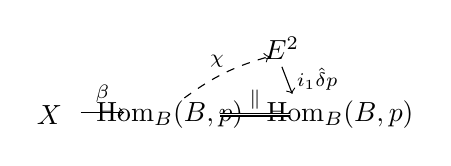
\begin{tikzpicture}[x=1.5em,y=1.5em]
  \node (E2) at (5.6,1.6) {$E^{2}$};
  \node (X)  at (0,0) {$X$};
  \node (H1) at (2.9,0) {$\mathrm{Hom}_{B}(B,p)$};
  \node (H2) at (7.0,0) {$\mathrm{Hom}_{B}(B,p)$};
  \draw[->] (0.75,0.05) -- node[above]{$\scriptstyle\qcor{\beta}$} (1.8,0.05);
  \draw[double] (4.1,0) -- (5.8,0);
  \node at (4.95,0.35) {$\scriptstyle\parallel$};
  \draw[->,dashed] (3.25,0.4) to[bend left=10] node[above,pos=0.4]{$\scriptstyle\qcor{\chi}$} (5.3,1.4);
  \draw[->] (5.6,1.15) -- (5.85,0.5);
  \node at (6.45,0.85) {$\scriptstyle i_{1}\hat{\delta}p$};
\end{tikzpicture}
\end{center}
对任意 $\qcor{\beta}\colon X\to\mathrm{Hom}_{B}(B,p)$ 都定义了一个绝对右提升，
从而由定理 5.1.7(ii)，任何 $\beta\colon b\Rightarrow pe$ 都容有一个 $p$-笛卡尔
提升。
\end{proof}

当 $p$ 是\trCartesianFibration{}时，我们把 \eqref{eq:right-comma-cone} 的泛%
笛卡尔箭头 $\qcor{\chi}\colon\mathrm{Hom}_{B}(B,p)\to E^{2}$ 称作%
\textbf{泛 $p$-笛卡尔提升}（generic $p$-cartesian lift）。

\begin{remark}[笛卡尔纤维化的纤维上的箭头作用]\label{rem:fiber-action}
\trCartesianFibration{}的底范畴中一支箭头在诸\trFiber{}上的作用可以描述如下。
考虑余定义域为 $B$ 的\trNaturalTransformation{} $\beta$，并作出 $p$ 在其定义域
函子与余定义域函子之上的诸\trFiber
\begin{center}
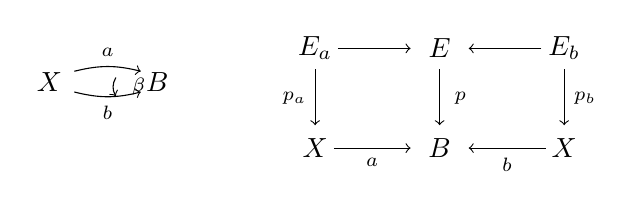
\begin{tikzpicture}[x=1.5em,y=1.5em]
  \begin{scope}[shift={(0,0.5)}]
  \node (B) at (2.6,0) {$B$};
  \node (X) at (0,0) {$X$};
  \draw[->] (0.6,0.25) to[bend left=14] node[above]{$\scriptstyle a$} (2.2,0.25);
  \draw[->] (0.6,-0.25) to[bend right=14] node[below]{$\scriptstyle b$} (2.2,-0.25);
  \draw[->] (1.6,0.1) to[bend right=30] (1.6,-0.35);
  \node at (2.15,-0.12) {$\scriptstyle\beta$};
  \end{scope}
  \begin{scope}[shift={(6.4,0)}]
  \node (Ea) at (0,1.3) {$E_{a}$};
  \node (E)  at (3.0,1.3) {$E$};
  \node (Eb) at (6.0,1.3) {$E_{b}$};
  \node (Xa) at (0,-1.1) {$X$};
  \node (Bm) at (3.0,-1.1) {$B$};
  \node (Xb) at (6.0,-1.1) {$X$};
  \draw[->] (0.55,1.3) -- (2.3,1.3);
  \draw[->] (5.45,1.3) -- (3.7,1.3);
  \draw[->] (0,0.8) -- (0,-0.55);
  \node at (-0.5,0.1) {$\scriptstyle p_{a}$};
  \draw[->] (3.0,0.8) -- (3.0,-0.55);
  \node at (3.5,0.1) {$\scriptstyle p$};
  \draw[->] (6.0,0.8) -- (6.0,-0.55);
  \node at (6.5,0.1) {$\scriptstyle p_{b}$};
  \draw[->] (0.45,-1.1) -- node[below]{$\scriptstyle a$} (2.3,-1.1);
  \draw[->] (5.55,-1.1) -- node[below]{$\scriptstyle b$} (3.7,-1.1);
  \node at (0.42,0.72) {$\scriptstyle\llcorner$};
  \node at (5.58,0.72) {$\scriptstyle\lrcorner$};
  \end{scope}
\end{tikzpicture}
\end{center}
定义\trFiber{} $E_{b}$ 的\trPullback{}方块可以像下左那样分解
\begin{center}
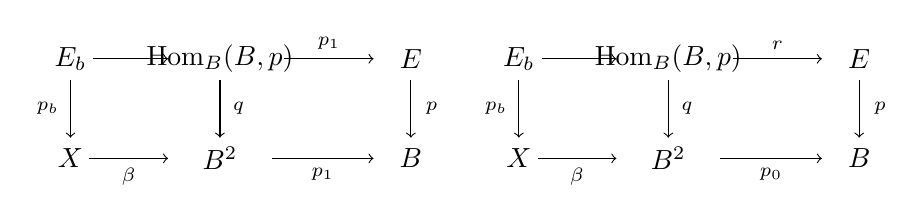
\begin{tikzpicture}[x=1.5em,y=1.5em]
  \begin{scope}[shift={(0,0)}]
  \node (Eb) at (0,1.4) {$E_{b}$};
  \node (H)  at (3.6,1.4) {$\mathrm{Hom}_{B}(B,p)$};
  \node (E)  at (8.2,1.4) {$E$};
  \node (X)  at (0,-1.0) {$X$};
  \node (B2) at (3.6,-1.0) {$B^{2}$};
  \node (B)  at (8.2,-1.0) {$B$};
  \draw[->] (0.55,1.4) -- (2.35,1.4);
  \draw[->] (5.15,1.4) -- node[above]{$\scriptstyle p_{1}$} (7.3,1.4);
  \draw[->] (0,0.9) -- (0,-0.5);
  \node at (-0.55,0.2) {$\scriptstyle p_{b}$};
  \draw[->] (3.6,0.9) -- (3.6,-0.5);
  \node at (4.05,0.2) {$\scriptstyle q$};
  \draw[->] (8.2,0.9) -- (8.2,-0.5);
  \node at (8.7,0.2) {$\scriptstyle p$};
  \draw[->] (0.45,-1.0) -- node[below]{$\scriptstyle\qcor{\beta}$} (2.35,-1.0);
  \draw[->] (4.85,-1.0) -- node[below]{$\scriptstyle p_{1}$} (7.3,-1.0);
  \node at (0.45,0.85) {$\scriptstyle\llcorner$};
  \node at (5.2,0.85) {$\scriptstyle\llcorner$};
  \end{scope}
  \begin{scope}[shift={(10.8,0)}]
  \node (Eb) at (0,1.4) {$E_{b}$};
  \node (H)  at (3.6,1.4) {$\mathrm{Hom}_{B}(B,p)$};
  \node (E)  at (8.2,1.4) {$E$};
  \node (X)  at (0,-1.0) {$X$};
  \node (B2) at (3.6,-1.0) {$B^{2}$};
  \node (B)  at (8.2,-1.0) {$B$};
  \draw[->] (0.55,1.4) -- (2.35,1.4);
  \draw[->] (5.15,1.4) -- node[above]{$\scriptstyle r$} (7.3,1.4);
  \draw[->] (0,0.9) -- (0,-0.5);
  \node at (-0.55,0.2) {$\scriptstyle p_{b}$};
  \draw[->] (3.6,0.9) -- (3.6,-0.5);
  \node at (4.05,0.2) {$\scriptstyle q$};
  \draw[->] (8.2,0.9) -- (8.2,-0.5);
  \node at (8.7,0.2) {$\scriptstyle p$};
  \draw[->] (0.45,-1.0) -- node[below]{$\scriptstyle\qcor{\beta}$} (2.35,-1.0);
  \draw[->] (4.85,-1.0) -- node[below]{$\scriptstyle p_{0}$} (7.3,-1.0);
  \node at (0.45,0.85) {$\scriptstyle\llcorner$};
  \end{scope}
\end{tikzpicture}
\end{center}
从而上右展示的矩形在定义 $E_{a}$ 的那个\trPullback{}之上定义了一个\trCone，诱导出
映射 $\beta^{*}\colon E_{b}\to E_{a}$。此矩形中顶部的水平函子复原了余定义域为
$\ell_{b}$ 的 $\beta$ 的 $p$-笛卡尔提升的定义域分量 $\beta^{*}(\ell_{b})$。这与
(5.0.1) 中给出的 $\beta^{*}\colon E_{b}\to E_{a}$ 的描述相吻合。
\end{remark}

\cref{lem:right-comma-cone-lift}可以加以扩充，给出\trCartesianFibration{}%
的一个内部刻画，其灵感来自 Street [118, 119, 121] 的一条类似结果，而后者又受
Gray [48] 论及他所称「Chevalley 判据」\footnote{Gray 把 [48, 3.11]——即%
\cref{thm:internal-characterization}的 $(i)\Leftrightarrow(ii)$ 等价在%
\trInfinityCosmos{} $\mathcal{C}at$ 中的特例——归功于 Claude Chevalley 1962 年
在 Berkeley 开设的一个讨论班的未发表讲义。}的先前工作所启发（另见 [131]）。我们
将会看到，\trCartesianFibration{}
$p\colon E\twoheadrightarrow B$ 的\trUniversalProperty{}可以由如下数据编码：由
恒同 2-胞腔诱导出的函子 $\Delta_{p}\colon E\to\mathrm{Hom}_{B}(B,p)$ 的某个合适
的\trRightAdjoint，或者把 $p$ 应用于余定义域为 $E$ 的\trGenericArrow{}而定义的
函子 $i_{1}\hat{\delta}p\colon E^{2}\to\mathrm{Hom}_{B}(B,p)$ 的某个合适的%
\trRightAdjoint。事实上，只要把定理 5.1.7 中 $p$-笛卡尔胞腔的诸刻画特化到%
\cref{lem:right-comma-cone-lift}所描述的泛情形，这条结果就相当容易地随之得出。

\begin{theorem}[笛卡尔纤维化的一个内部刻画]\label{thm:internal-characterization}
对一条\trIsofibration{} $p\colon E\twoheadrightarrow B$，下列诸条等价：
\begin{enumerate}[label=(\roman*)]
\item $p\colon E\twoheadrightarrow B$ 定义了一条\trCartesianFibration。
\item 函子 $i_{1}\hat{\delta}p\colon E^{2}\to\mathrm{Hom}_{B}(B,p)$
容有一个右伴随右逆：%
\footnote{由引理 3.6.9，这样的伴随可以矫正为在 $\mathrm{Hom}_{B}(B,p)$
之上纤维化的伴随；故 $\qcor{\chi}\colon\mathrm{Hom}_{B}(B,p)\to E^{2}$
可解释为「$E^{2}$ 在 $\mathrm{Hom}_{B}(B,p)$ 之上由 $\qcor{\chi}$
切出的一个\trTerminal{}\trElement{}」（见定义 3.6.8）。}
\begin{center}
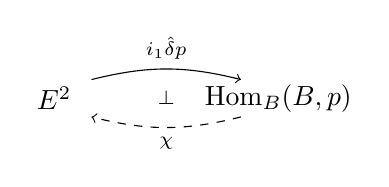
\begin{tikzpicture}[x=1.5em,y=1.5em]
  \node (E2) at (0,0) {$E^{2}$};
  \node (H)  at (5.4,0) {$\mathrm{Hom}_{B}(B,p)$};
  \draw[->] (0.9,0.45) to[bend left=14] node[above]{$\scriptstyle i_{1}\hat{\delta}p$} (4.5,0.45);
  \node at (2.7,0) {$\scriptstyle\perp$};
  \draw[->,dashed] (4.5,-0.45) to[bend left=14] node[below]{$\scriptstyle\qcor{\chi}$} (0.9,-0.45);
\end{tikzpicture}
\end{center}
\item 函子 $\Delta_{p}\colon E\to\mathrm{Hom}_{B}(B,p)$ 容有一个 $B$ 上的%
\trRightAdjoint：\footnote{由引理 3.5.9，$\Delta_{p}\simeq\qcor{\mathrm{id}_{p}}$
本身就是余定义域投影函子 $p_{1}\colon\mathrm{Hom}_{B}(B,p)\to E$ 在 $E$ 之上、
从而也在 $B$ 之上的\trRightAdjoint。由于伴随 $p_{1}\dashv\Delta_{p}$ 的%
\trCounit{}是一个\trIsomorphism，故只要 (iii) 中所假设的伴随存在（见引理
B.3.9），形式上即可推出伴随 $\Delta_{p}\dashv r$ 的\trUnit{}也必是%
\trIsomorphism。于是 $r$ 定义了 $\Delta_{p}$ 在 $B$ 之上的一个右伴随左逆。}
\begin{center}
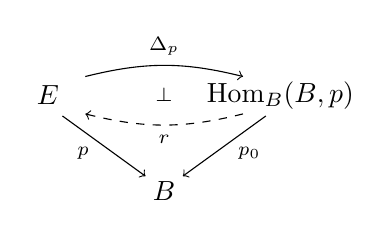
\begin{tikzpicture}[x=1.5em,y=1.5em]
  \node (E) at (0,0) {$E$};
  \node (H) at (5.6,0) {$\mathrm{Hom}_{B}(B,p)$};
  \draw[->] (0.9,0.45) to[bend left=14] node[above]{$\scriptstyle\Delta_{p}$} (4.7,0.45);
  \node at (2.8,0) {$\scriptstyle\perp$};
  \draw[->,dashed] (4.7,-0.45) to[bend left=14] node[below]{$\scriptstyle r$} (0.9,-0.45);
  \node (B) at (2.8,-2.3) {$B$};
  \draw[->] (0.35,-0.5) -- (2.35,-1.95);
  \node at (0.85,-1.4) {$\scriptstyle p$};
  \draw[->] (5.25,-0.5) -- (3.25,-1.95);
  \node at (4.85,-1.4) {$\scriptstyle p_{0}$};
\end{tikzpicture}
\end{center}
\end{enumerate}
\end{theorem}

正如证明所揭示的，(iii) 的\trRightAdjoint{}是 \eqref{eq:right-comma-cone} 的泛%
$p$-笛卡尔提升 $\chi$ 的定义域分量，而 $\chi$ 可复原为 $p_{1}\epsilon$，其中
$\epsilon$ 是\trFiberedAdjunction{} $\Delta_{p}\dashv r$ 的\trCounit。由\trOneCellInduction，
泛笛卡尔提升 $\chi$ 可以由一个函子 $\qcor{\chi}\colon\mathrm{Hom}_{B}(B,p)\to E^{2}$
表示，而这便定义了 (ii) 的\trRightAdjoint。

\begin{proof}
我们证明 $(i)\Leftrightarrow(ii)$ 与 $(i)\Leftrightarrow(iii)$。

\textbf{(i)$\Leftrightarrow$(ii)：}由定理 5.1.7(ii) 与%
\cref{lem:right-comma-cone-lift}，
$p\colon E\twoheadrightarrow B$ 是\trCartesianFibration，当且仅当
$i_{1}\hat{\delta}p\colon E^{2}\to\mathrm{Hom}_{B}(B,p)$ 容有一个定义出绝对右
提升图的\trSection：
\begin{center}
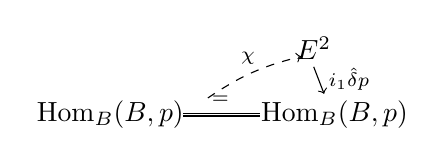
\begin{tikzpicture}[x=1.5em,y=1.5em]
  \node (E2) at (4.9,1.6) {$E^{2}$};
  \node (H1) at (0,0) {$\mathrm{Hom}_{B}(B,p)$};
  \node (H2) at (5.4,0) {$\mathrm{Hom}_{B}(B,p)$};
  \draw[double] (1.75,0) -- (3.6,0);
  \node at (2.65,0.35) {$\scriptstyle=$};
  \draw[->,dashed] (2.35,0.4) to[bend left=10] node[above,pos=0.45]{$\scriptstyle\qcor{\chi}$} (4.6,1.4);
  \draw[->] (4.9,1.15) -- (5.15,0.5);
  \node at (5.75,0.85) {$\scriptstyle i_{1}\hat{\delta}p$};
\end{tikzpicture}
\end{center}
由引理 2.3.7，这样的绝对右提升定义了一个余单位为恒同的伴随
$i_{1}\hat{\delta}p\dashv\qcor{\chi}$。反之，若 $i_{1}\hat{\delta}p\dashv\qcor{\chi}$
带有可逆余单位，则由于左伴随是一条\trIsofibration，它可以被矫正为一个纤维化
伴随，其中 $\qcor{\chi}$ 定义了一个严格\trSection{}而余单位是恒同。由引理
2.3.7，$\qcor{\chi}$ 于是定义了恒同函子穿过 $i_{1}\hat{\delta}p$ 的一个绝对右
提升，这就证明 $p$ 是一条\trCartesianFibration。

\textbf{(i)$\Leftrightarrow$(iii)：}若 $p\colon E\twoheadrightarrow B$ 是%
\trInfinityCosmos{} $\mathcal{K}$中的一条\trCartesianFibration，则由定理
5.1.7(iii) 存在绝对右提升图表
\begin{center}
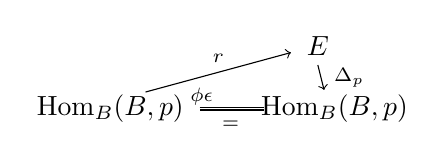
\begin{tikzpicture}[x=1.5em,y=1.5em]
  \node (E)  at (5.0,1.5) {$E$};
  \node (H1) at (0,0) {$\mathrm{Hom}_{B}(B,p)$};
  \node (H2) at (5.4,0) {$\mathrm{Hom}_{B}(B,p)$};
  \draw[->] (0.85,0.4) -- node[above,pos=0.5]{$\scriptstyle r$} (4.35,1.35);
  \node at (2.2,0.3) {$\scriptstyle\phi\epsilon$};
  \draw[->] (5.0,1.05) -- (5.15,0.45);
  \node at (5.75,0.75) {$\scriptstyle\Delta_{p}$};
  \draw[double] (2.15,0) -- (3.7,0);
  \node at (2.9,-0.38) {$\scriptstyle=$};
\end{tikzpicture}
\end{center}
满足 $p_{0}\epsilon=\mathrm{id}_{p_{0}}$。由命题 3.6.2，我们可以把 $\epsilon$
提升为\trSliceInfinityCosmos{} $\mathcal{K}_{/B}$ 中的一个%
\trNaturalTransformation。在
$\mathcal{K}_{/B}$ 中应用引理 2.3.7，可见 $r$ 定义了 $\Delta_{p}$ 的一个纤维化%
\trRightAdjoint。反之，若给定一个 $B$ 上的\trFiberedAdjunction，我们可以应用遗忘 2-函子
$\hbar(\mathcal{K}_{/B})\to\hbar\mathcal{K}$ 得到一个伴随\footnote{回忆非例
1.3.6：遗忘函子 $\mathcal{K}_{/B}\to\mathcal{K}$ 不是宇宙论的。尽管如此，%
\trInfinityCosmos{}之间的任何\trSimplicialFunctor{}都会下降为其%
\trHomotopyTwoCategory{}之间
的一个\trTwoFunctor，而这正是此处所需的全部。}
\begin{center}
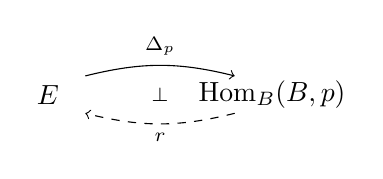
\begin{tikzpicture}[x=1.5em,y=1.5em]
  \node (E) at (0,0) {$E$};
  \node (H) at (5.4,0) {$\mathrm{Hom}_{B}(B,p)$};
  \draw[->] (0.9,0.45) to[bend left=14] node[above]{$\scriptstyle\Delta_{p}$} (4.5,0.45);
  \node at (2.7,0) {$\scriptstyle\perp$};
  \draw[->,dashed] (4.5,-0.45) to[bend left=14] node[below]{$\scriptstyle r$} (0.9,-0.45);
\end{tikzpicture}
\end{center}
然后再应用引理 2.3.7 得出：\trCounit{} $\epsilon$ 定义了恒同穿过 $\Delta_{p}$ 的
一个绝对右提升。由于余单位在「遗忘伴随在 $B$ 之上纤维化」这一过程中保持不变，
我们仍有 $p_{0}\epsilon=\mathrm{id}_{p_{0}}$，正如所需。
\end{proof}

\trCartesianFibration{}的例子早就该登场了。

\begin{proposition}[定义域投影纤维化]\label{prop:domain-projection-fibration}
对任意\trInfinityCategory{} $A$，定义域投影函子
$p_{0}\colon A^{2}\twoheadrightarrow A$ 定义了
一条\trCartesianFibration。此外，余定义域为 $A^{2}$ 的\trNaturalTransformation{}
$\psi$ 是 $p_{0}$-\trCartesian，当且仅当 $p_{1}\psi$ 可逆。
\end{proposition}

在给出证明之前，我们先解释其想法。\trNaturalTransformation
\begin{center}
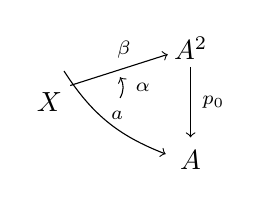
\begin{tikzpicture}[x=1.5em,y=1.5em]
  \node (A2) at (3.4,1.3) {$A^{2}$};
  \node (X)  at (0,0) {$X$};
  \node (A)  at (3.4,-1.4) {$A$};
  \draw[->] (0.5,0.4) -- node[above,pos=0.55]{$\scriptstyle\qcor{\beta}$} (2.85,1.15);
  \draw[->] (3.4,0.85) -- (3.4,-0.85);
  \node at (3.95,0) {$\scriptstyle p_{0}$};
  \draw[->] (0.35,0.75) to[bend right=18] node[above,pos=0.6]{$\scriptstyle a$} (2.8,-1.25);
  \draw[->] (1.7,0.1) to[bend right=30] (1.7,0.6);
  \node at (2.25,0.35) {$\scriptstyle\alpha$};
\end{tikzpicture}
\end{center}
定义了 $\mathrm{hFun}(X,A)$ 中一对可复合的 2-胞腔 $\alpha\colon a\Rightarrow x$
与 $\beta\colon x\Rightarrow y$。复合二者即诱导出一个 2-胞腔
\cellpair{X}{A^{2}}{\qcor{\beta\circ\alpha}}{\qcor{\beta}}{\psi}
它表示 $\mathrm{hFun}(X,A)$ 中的交换方块
\begin{center}
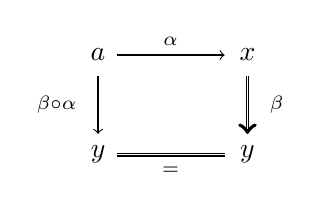
\begin{tikzpicture}[x=1.5em,y=1.5em]
  \node (a)  at (0,1.2) {$a$};
  \node (x)  at (3.6,1.2) {$x$};
  \node (y1) at (0,-1.2) {$y$};
  \node (y2) at (3.6,-1.2) {$y$};
  \draw[->] (0.45,1.2) -- node[above]{$\scriptstyle\alpha$} (3.05,1.2);
  \draw[->] (0,0.7) -- (0,-0.7);
  \node at (-1.0,0) {$\scriptstyle\beta\circ\alpha$};
  \draw[double,->] (3.6,0.7) -- (3.6,-0.7);
  \node at (4.3,0) {$\scriptstyle\beta$};
  \draw[double] (0.45,-1.2) -- (3.05,-1.2);
  \node at (1.75,-1.6) {$\scriptstyle=$};
\end{tikzpicture}
\end{center}
使得 $p_{0}\psi=\alpha$（正如所需）且 $p_{1}\psi=\mathrm{id}$。

\begin{proof}
我们使用\cref{thm:internal-characterization}(ii)，通过为函子
\begin{center}
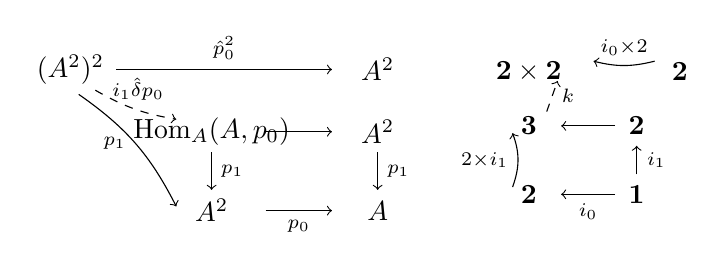
\begin{tikzpicture}[x=1.5em,y=1.5em]
  \begin{scope}[shift={(0,0)}]
  \node (A22) at (0,2.4) {$(A^{2})^{2}$};
  \node (A2t) at (7.4,2.4) {$A^{2}$};
  \node (H)   at (3.4,0.9) {$\mathrm{Hom}_{A}(A,p_{0})$};
  \node (A2m) at (7.4,0.9) {$A^{2}$};
  \node (A2b) at (3.4,-1.0) {$A^{2}$};
  \node (A)   at (7.4,-1.0) {$A$};
  \draw[->] (1.1,2.4) -- node[above]{$\scriptstyle\hat{p}_{0}^{2}$} (6.3,2.4);
  \draw[->,dashed] (0.6,1.9) to[bend right=10] node[above,pos=0.55]{$\scriptstyle i_{1}\hat{\delta}p_{0}$} (2.55,1.2);
  \draw[->] (4.7,0.9) -- (6.3,0.9);
  \node at (5.15,1.2) {$\scriptstyle\llcorner$};
  \draw[->] (0.2,1.8) to[bend left=14] node[left,pos=0.5]{$\scriptstyle p_{1}$} (2.55,-0.9);
  \draw[->] (3.4,0.4) -- (3.4,-0.5);
  \node at (3.9,-0.05) {$\scriptstyle p_{1}$};
  \draw[->] (7.4,0.4) -- (7.4,-0.5);
  \node at (7.9,-0.05) {$\scriptstyle p_{1}$};
  \draw[->] (4.7,-1.0) -- node[below]{$\scriptstyle p_{0}$} (6.3,-1.0);
  \end{scope}
  \begin{scope}[shift={(10.0,0)},x=1.3em,y=1.3em]
  \node (tt)  at (1.2,2.7) {$\qcTwo\times\qcTwo$};
  \node (t2a) at (5.4,2.7) {$\qcTwo$};
  \node (t3)  at (1.2,1.2) {$\qcThree$};
  \node (t2b) at (4.2,1.2) {$\qcTwo$};
  \node (t2c) at (1.2,-0.7) {$\qcTwo$};
  \node (t1)  at (4.2,-0.7) {$\qcOne$};
  \draw[->] (4.7,3.0) to[bend left=14] node[above,pos=0.5]{$\scriptstyle i_{0}\times 2$} (3.0,3.0);
  \draw[->,dashed] (1.7,1.6) -- node[right,pos=0.5]{$\scriptstyle k$} (2.0,2.45);
  \draw[->] (3.6,1.2) -- (2.1,1.2);
  \draw[->] (0.75,-0.5) to[bend right=20] node[left,pos=0.5]{$\scriptstyle 2\times i_{1}$} (0.75,1.0);
  \draw[->] (4.2,-0.15) -- (4.2,0.65);
  \node at (4.75,0.25) {$\scriptstyle i_{1}$};
  \draw[->] (3.6,-0.7) -- node[below]{$\scriptstyle i_{0}$} (2.1,-0.7);
  \end{scope}
\end{tikzpicture}
\end{center}
构造一个合适的伴随来证明 $p_{0}$ 是\trCartesian，该函子由与右上所展示的诸 1-范畴作%
\trCotensor{}而定义。\footnote{\trCotensor{} $A^{(-)}$ 把\trSimplicialSet{}的%
\trPushout{}送到\trInfinityCategory{}的\trPullback，而\trSimplicialSet{}
$2\sqcup_{0}2$ 的\trPushout{}是 $\wedge=\Lambda^{1}[2]$，而非
$3=\Delta[2]$。然而，由于\trInfinityCategory{}之间的\trEquivalence{}
$A^{3}\simeq A^{\wedge}$，作此处所指的替换并无妨碍。}

要为映射 $i_{1}\hat{\delta}p_{0}$ 构造一个右伴随右逆，只需为 1-范畴的包含
$k\colon\qcThree\hookrightarrow\qcTwo\times\qcTwo$——其像为
$(0,0)\to(0,1)\to(1,1)$——构造一个左伴随左逆。左伴随
$\ell\colon\qcTwo\times\qcTwo\to\qcThree$ 在 $\qcThree$ 的像上是左逆，并把
$(1,0)$ 送到 $\qcThree$ 的\trTerminal{}元素：
\[
\qcTwo\times\qcTwo\ni
\left\{\begin{array}{ccc}
(0,0) & \longrightarrow & (0,1)\\
\downarrow & & \downarrow\\
(1,0) & \longrightarrow & (1,1)
\end{array}\right\}
\;\overset{\ell}{\longmapsto}\;
\left\{\begin{array}{ccc}
0 & \longrightarrow & 1\\
\downarrow & & \downarrow\\
2 & = & 2
\end{array}\right\}
\in\qcThree
\]
现在
\begin{center}
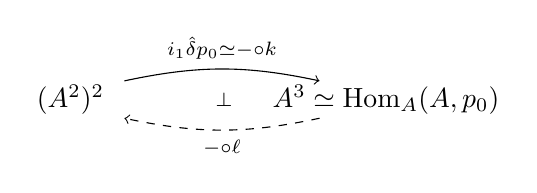
\begin{tikzpicture}[x=1.5em,y=1.5em]
  \node (A22) at (0,0) {$(A^{2})^{2}$};
  \node (A3)  at (7.6,0) {$A^{3}\simeq\mathrm{Hom}_{A}(A,p_{0})$};
  \draw[->] (1.3,0.45) to[bend left=12] node[above]{$\scriptstyle i_{1}\hat{\delta}p_{0}\simeq-\circ k$} (6.0,0.45);
  \node at (3.7,0) {$\scriptstyle\perp$};
  \draw[->,dashed] (6.0,-0.45) to[bend left=12] node[below]{$\scriptstyle-\circ\ell$} (1.3,-0.45);
\end{tikzpicture}
\end{center}
定义了所求的右伴随右逆。

$p_{0}$-笛卡尔变换的刻画由定理 5.1.7(ii) 得出。对任意箭头
$\qcor{\psi}\colon X\to A^{2}$，左下的交换三角形穿过由该伴随定义的绝对提升图
分解，而 $\qcor{\psi}$ 是 $p_{0}$-\trCartesian，当且仅当诱导出的%
\trNaturalTransformation{} $\zeta$ 可逆。
\begin{center}
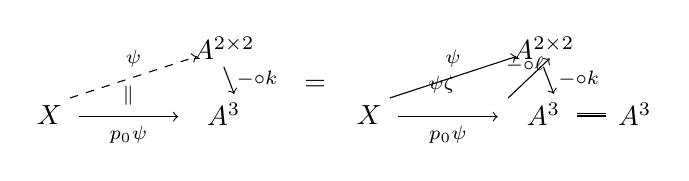
\begin{tikzpicture}[x=1.5em,y=1.5em]
  \begin{scope}[shift={(0,0)}]
  \node (A22) at (4.2,1.6) {$A^{2\times 2}$};
  \node (X)   at (0,0) {$X$};
  \node (A3)  at (4.2,0) {$A^{3}$};
  \draw[->,dashed] (0.5,0.4) -- node[above,pos=0.5]{$\scriptstyle\qcor{\psi}$} (3.55,1.4);
  \node at (1.9,0.45) {$\scriptstyle\parallel$};
  \draw[->] (0.7,-0.05) -- node[below]{$\scriptstyle\qcor{p_{0}\psi}$} (3.1,-0.05);
  \draw[->] (4.2,1.15) -- (4.45,0.5);
  \node at (5.0,0.85) {$\scriptstyle-\circ k$};
  \node at (6.4,0.7) {$=$};
  \end{scope}
  \begin{scope}[shift={(7.7,0)}]
  \node (A22) at (4.2,1.6) {$A^{2\times 2}$};
  \node (X)   at (0,0) {$X$};
  \node (A3)  at (4.2,0) {$A^{3}$};
  \node (A3b) at (6.4,0) {$A^{3}$};
  \draw[->] (0.5,0.4) -- node[above,pos=0.5]{$\scriptstyle\qcor{\psi}$} (3.55,1.4);
  \node at (1.75,0.72) {$\scriptstyle\psi\zeta$};
  \draw[->] (0.7,-0.05) -- node[below]{$\scriptstyle\qcor{p_{0}\psi}$} (3.1,-0.05);
  \draw[->] (3.35,0.4) -- node[above,pos=0.4]{$\scriptstyle-\circ\ell$} (4.35,1.35);
  \draw[double] (5.0,0) -- (5.7,0);
  \draw[->] (4.2,1.15) -- (4.45,0.5);
  \node at (5.05,0.85) {$\scriptstyle-\circ k$};
  \end{scope}
\end{tikzpicture}
\end{center}
若 $\zeta$ 是一个\trIsomorphism，则 $\qcor{\psi}$ 与沿 $\ell$ 取限制所得像中的
一支箭头同构，于是其余定义域分量必可逆。反之，若 $p_{1}\psi$ 可逆，则由定理
5.1.7(ii)，欲证 $\psi$ 是 $p_{0}$-\trCartesian，只需证 $\zeta$ 是\trIsomorphism。
由\trTwoCellConservativity{}的两次应用，只需证：以 $\qcTwo\times\qcTwo$ 的每个
元素为指标的 $\zeta$ 的四个分量都可逆。由于 $\zeta$ 沿 $k$ 限制为恒同，这些分量
中有三个必为恒同，而第四个分量
\begin{center}
\begin{tikzpicture}[x=1.5em,y=1.5em]
  \node (X)   at (0,0) {$X$};
  \node (A22) at (5.0,0) {$A^{2\times 2}$};
  \node (A)   at (10.0,0) {$A$};
  \draw[->] (0.75,0.32) to[bend left=18] node[above]{$\scriptstyle\qcor{\psi}$} (4.2,0.32);
  \draw[->] (0.75,-0.32) to[bend right=18] node[below]{$\scriptstyle\qcor{p_{0}\psi}\vert_{\ell}$} (4.2,-0.32);
  \draw[->] (2.5,0.15) to[bend right=32] (2.5,-0.25);
  \node at (3.35,-0.02) {$\scriptstyle\psi\zeta$};
  \draw[->] (6.0,0) -- node[above]{$\scriptstyle P_{(1,0)}$} (9.1,0);
\end{tikzpicture}
\end{center}
在 $\mathrm{hFun}(X,A)$ 中等于 $p_{1}\psi$。
\end{proof}

对容许\trPullback{}的\trInfinityCategory（见定义 4.3.8），余定义域投影函子也
定义了一条\trCartesianFibration：

\begin{proposition}[余定义域投影纤维化]\label{prop:codomain-projection-fibration}
设 $A$ 是容许\trPullback{}的\trInfinityCategory。则余定义域投影函子
$p_{1}\colon A^{2}\twoheadrightarrow A$ 是一条\trCartesianFibration，且诸
$p_{1}$-笛卡尔箭头
恰是\trPullback{}方块。
\end{proposition}

\begin{proof}
我们经由\cref{thm:internal-characterization}(ii)，为函子 $i_{1}\hat{\delta}p_{1}$
寻找一个右伴随右逆，该函子由下左定义，即把 $A^{(-)}$ 应用于下右所展示的单纯集
图表：\footnote{原书此边印作 $p_{0}$，依 $\mathrm{Hom}_{A}(A,p_{1})$ 之拉回刻画
当作 $p_{1}$，径改。——译者注}
\begin{center}
\begin{tikzpicture}[x=1.5em,y=1.5em]
  \begin{scope}[shift={(0,0)}]
  \node (A22) at (0,2.4) {$(A^{2})^{2}$};
  \node (A2t) at (7.4,2.4) {$A^{2}$};
  \node (H)   at (3.4,0.9) {$\mathrm{Hom}_{A}(A,p_{1})$};
  \node (A2m) at (7.4,0.9) {$A^{2}$};
  \node (A2b) at (3.4,-1.0) {$A^{2}$};
  \node (A)   at (7.4,-1.0) {$A$};
  \draw[->] (1.1,2.4) -- node[above]{$\scriptstyle\hat{p}_{1}^{2}$} (6.3,2.4);
  \draw[->,dashed] (0.6,1.9) to[bend right=10] node[above,pos=0.55]{$\scriptstyle i_{1}\hat{\delta}p_{1}$} (2.55,1.2);
  \draw[->] (4.7,0.9) -- (6.3,0.9);
  \node at (5.15,1.2) {$\scriptstyle\llcorner$};
  \draw[->] (0.2,1.8) to[bend left=14] node[left,pos=0.5]{$\scriptstyle p_{1}$} (2.55,-0.9);
  \draw[->] (3.4,0.4) -- (3.4,-0.5);
  \node at (3.9,-0.05) {$\scriptstyle p_{1}$};
  \draw[->] (7.4,0.4) -- (7.4,-0.5);
  \node at (7.9,-0.05) {$\scriptstyle p_{1}$};
  \draw[->] (4.7,-1.0) -- node[below]{$\scriptstyle p_{1}$} (6.3,-1.0);
  \end{scope}
  \begin{scope}[shift={(10.0,0)},x=1.3em,y=1.3em]
  \node (tt)  at (1.2,2.7) {$\qcTwo\times\qcTwo$};
  \node (t2a) at (5.4,2.7) {$\qcTwo$};
  \node (lc)  at (1.2,1.2) {$\lrcorner$};
  \node (t2b) at (4.2,1.2) {$\qcTwo$};
  \node (t2c) at (1.2,-0.7) {$\qcTwo$};
  \node (t1)  at (4.2,-0.7) {$\qcOne$};
  \draw[->] (4.7,3.0) to[bend left=14] node[above,pos=0.5]{$\scriptstyle 1\times 2$} (3.0,3.0);
  \draw[->,dashed] (1.7,1.6) -- (2.0,2.45);
  \draw[->] (3.6,1.2) -- (2.1,1.2);
  \draw[->] (0.75,-0.5) to[bend right=20] node[left,pos=0.5]{$\scriptstyle 2\times 1$} (0.75,1.0);
  \draw[->] (4.2,-0.15) -- (4.2,0.65);
  \node at (4.75,0.25) {$\scriptstyle i_{1}$};
  \draw[->] (3.6,-0.7) -- node[below]{$\scriptstyle i_{0}$} (2.1,-0.7);
  \end{scope}
\end{tikzpicture}
\end{center}
这正是由推论 4.3.5 所提供的：
\[
\bigl(A^{2}\bigr)^{2}\simeq A^{\square}
\;\begin{array}{c}
\xrightarrow{\ \mathrm{res}\ }\\
\perp\\
\xleftarrow[\ \mathrm{ran}\ ]{}
\end{array}\;
A^{\lrcorner}\simeq\mathrm{Hom}_{A}(A,p_{1})
\]
把定义 4.3.8 与定理 5.1.7(ii) 相比较，即可见诸 $p_{1}$-笛卡尔箭头与\trPullback{}%
方块重合。
\end{proof}

\trCartesianFibration{}还有第四种等价定义，我们本可以把它添入%
\cref{thm:internal-characterization}，只不过它是\trCartesianFibration{}的「外部
刻画」——完全在\trHomotopyTwoCategory{}的框架内陈述——而非「内部刻画」；便于
证明\trCartesianFibration{}在\trCosmologicalFunctor{}下保持的，正是这个外部刻画。

\begin{proposition}\label{prop:external-characterization}
一条\trIsofibration{} $p\colon E\twoheadrightarrow B$ 是\trCartesianFibration，
当且仅当任何\trNaturalTransformation{} $\beta\colon b\Rightarrow pe$ 都容有一个
提升 $\chi_{\beta}\colon e'\Rightarrow e$
\begin{center}
\begin{tikzpicture}[x=1.5em,y=1.5em]
  \begin{scope}[shift={(0,0)}]
  \node (E) at (2.6,1.1) {$E$};
  \node (X) at (0,1.1) {$X$};
  \node (B) at (2.6,-0.9) {$B$};
  \draw[->] (0.6,1.35) to[bend left=14] node[above]{$\scriptstyle e$} (2.2,1.35);
  \draw[->] (2.6,0.7) -- (2.6,-0.45);
  \node at (3.05,0.1) {$\scriptstyle p$};
  \draw[->] (0.35,0.75) to[bend right=18] node[below,pos=0.5]{$\scriptstyle b$} (2.15,-0.95);
  \draw[->] (1.95,0.5) to[bend right=30] (1.95,0.95);
  \node at (1.25,0.72) {$\scriptstyle\beta$};
  \node at (4.4,0.1) {$=$};
  \end{scope}
  \begin{scope}[shift={(5.6,0)}]
  \node (E) at (2.6,1.1) {$E$};
  \node (X) at (0,1.1) {$X$};
  \node (B) at (2.6,-0.9) {$B$};
  \draw[->] (0.6,1.35) to[bend left=14] node[above]{$\scriptstyle e$} (2.2,1.35);
  \draw[->] (0.6,0.85) to[bend right=14] node[below]{$\scriptstyle e'$} (2.2,0.85);
  \draw[->] (2.6,0.7) -- (2.6,-0.45);
  \node at (3.05,0.1) {$\scriptstyle p$};
  \draw[->] (1.95,0.55) to[bend right=30] (1.95,1.0);
  \node at (1.35,0.78) {$\scriptstyle\chi_{\beta}$};
  \end{scope}
\end{tikzpicture}
\end{center}
使得对任何\trFunctor{} $f\colon Y\to X$，2-胞腔 $\chi_{\beta}f$ 在%
\trHomotopyTwoCategory{}中满足下列性质：
\begin{enumerate}[label=(\roman*)]
\item \textbf{归纳：}给定任意 2-胞腔 $\tau\colon e''\Rightarrow ef$ 与
$\gamma\colon pe''\Rightarrow pe'f$，使得 $p\tau=\beta f\cdot\gamma$，则存在
$\gamma$ 的一个\trLifting{} $\bar{\gamma}\colon e''\Rightarrow e'f$，使得
$\tau=\chi_{\beta}f\cdot\bar{\gamma}$。
\item \textbf{保守性：}$\chi_{\beta}f$ 的任何纤维化自同态皆可逆：对任何满足
$\chi_{\beta}f\cdot\zeta=\chi_{\beta}f$ 且 $p\zeta=\mathrm{id}_{pe'f}$ 的 2-胞腔
$\zeta\colon e'f\Rightarrow e'f$，$\zeta$ 可逆。
\end{enumerate}
此外，在这些假设之下，余定义域为 $E$ 的\trNaturalTransformation{}
$\psi\colon e'\Rightarrow e$ 是 $p$-\trCartesian，当且仅当 $\psi$ 在
$f=\mathrm{id}$ 的情形下满足归纳与保守性条件。
\end{proposition}

为在证明中保持条理，我们把满足条件 (i) 与 (ii) 的\trNaturalTransformation{}
$\psi\colon e'\Rightarrow e$ 称作\emph{弱 $p$-笛卡尔变换}。我们将论证：当 $p$
是\trCartesianFibration{}时，弱 $p$-笛卡尔变换类与 $p$-笛卡尔变换类相重合。

\begin{proof}
若 $p\colon E\twoheadrightarrow B$ 是\trCartesianFibration，则任何
$\beta\colon b\Rightarrow pe$ 都容有一个 $p$-笛卡尔提升
$\chi_{\beta}\colon\beta^{*}e\Rightarrow e$。由引理 5.1.4，沿任何函子的限制
$\chi_{\beta}f$ 仍是 $p$-笛卡尔变换。由命题 5.1.13，这个 $\chi_{\beta}f$ 便满足
归纳与保守性性质。事实上，命题 5.1.13 更一般地表明：任何 $p$-笛卡尔变换都是弱
$p$-\trCartesian。

反之，设 $p\colon E\twoheadrightarrow B$ 满足题设。我们将利用与 $p$ 之上的右
逗号锥 $\phi$ 的提升
\begin{center}
\begin{tikzpicture}[x=1.5em,y=1.5em]
  \begin{scope}[shift={(0,0)}]
  \node (H) at (0,1.1) {$\mathrm{Hom}_{B}(B,p)$};
  \node (E) at (4.0,1.1) {$E$};
  \node (B) at (4.0,-1.2) {$B$};
  \draw[->] (1.15,1.4) to[bend left=10] node[above]{$\scriptstyle p_{1}$} (3.4,1.4);
  \draw[->] (4.0,0.7) -- (4.0,-0.7);
  \node at (4.55,0) {$\scriptstyle p$};
  \draw[->] (0.8,0.7) to[bend right=24] (3.45,-1.2);
  \node at (0.95,-0.85) {$\scriptstyle p_{0}$};
  \draw[->] (1.7,0.4) to[bend right=30] (1.7,0.95);
  \node at (2.25,0.68) {$\scriptstyle\phi$};
  \node at (5.7,0.1) {$=$};
  \end{scope}
  \begin{scope}[shift={(7.2,0)}]
  \node (H) at (0,1.1) {$\mathrm{Hom}_{B}(B,p)$};
  \node (E) at (4.0,1.1) {$E$};
  \node (B) at (4.0,-1.2) {$B$};
  \draw[->] (1.15,1.4) to[bend left=10] node[above]{$\scriptstyle p_{1}$} (3.4,1.4);
  \draw[->] (1.15,0.85) -- (3.4,0.85);
  \node at (0.85,0.4) {$\scriptstyle r$};
  \draw[->] (4.0,0.7) -- (4.0,-0.7);
  \node at (4.55,0) {$\scriptstyle p$};
  \draw[->] (2.15,0.55) to[bend right=30] (2.15,1.0);
  \node at (2.7,0.78) {$\scriptstyle\chi$};
  \end{scope}
\end{tikzpicture}
\end{center}
及其诸限制相关联的归纳与保守性性质，来构造\cref{thm:internal-characterization}(iii)
的数据。

首先，我们把归纳性质应用于 $\chi\Delta_{p}\colon r\Delta_{p}\Rightarrow\mathrm{id}_{E}$，
诱导出一个 2-胞腔 $\eta\colon\mathrm{id}_{E}\Rightarrow r\Delta_{p}$，使得
$p\eta=\mathrm{id}_{p}$ 且 $\chi\Delta_{p}\cdot\eta=\mathrm{id}$。由构造，
$\eta\cdot\chi\Delta_{p}$ 定义了 $\chi\Delta_{p}$ 的一个纤维化自同构，故由保守性
性质必可逆。于是，纤维化 2-胞腔 $\eta$ 是 $\chi\Delta_{p}$ 的逆同构。

我们由 2-胞腔归纳，从 2-胞腔对 $p_{1}\epsilon=\chi$ 与 $p_{0}\epsilon=\mathrm{id}$
诱导出\trCounit{} $\epsilon\colon\Delta_{p}r\Rightarrow\mathrm{id}$。由于
$\epsilon\Delta_{p}$ 由一对可逆 2-胞腔诱导而来，由\trTwoCellConservativity{}它必
是\trIsomorphism。2-胞腔 $r\epsilon$ 也可看出是可逆的，理由是与水平复合相关联的
须化方块的自然性：
\begin{center}
\begin{tikzpicture}[x=1.5em,y=1.5em]
  \begin{scope}[shift={(0,0)}]
  \node (E)  at (3.4,1.5) {$E$};
  \node (H1) at (0,0) {$\mathrm{Hom}_{B}(B,p)$};
  \node (H2) at (5.2,0) {$\mathrm{Hom}_{B}(B,p)$};
  \draw[->] (0.85,0.4) -- node[above,pos=0.5]{$\scriptstyle r$} (2.9,1.35);
  \node at (1.65,0.3) {$\scriptstyle\phi\epsilon$};
  \draw[->] (3.8,1.25) -- (4.75,0.35);
  \node at (4.8,0.95) {$\scriptstyle\Delta_{p}$};
  \draw[double] (1.9,0) -- (3.6,0);
  \end{scope}
  \node at (7.3,0.7) {$\rightsquigarrow$};
  \begin{scope}[shift={(8.3,0)}]
  \node (H) at (0,0.9) {$\mathrm{Hom}_{B}(B,p)$};
  \node (E) at (3.6,0.9) {$E$};
  \draw[->] (0.7,1.15) to[bend left=10] node[above]{$\scriptstyle p_{1}$} (2.9,1.15);
  \draw[->] (0.7,0.55) -- (2.9,0.55);
  \node at (0.5,-0.05) {$\scriptstyle r$};
  \draw[->] (1.75,0.95) to[bend right=30] (1.75,0.5);
  \node at (2.3,0.72) {$\scriptstyle\chi$};
  \end{scope}
  \node at (13.4,0.7) {$\rightsquigarrow$};
  \begin{scope}[shift={(14.6,0)}]
  \node (rdr) at (0,1.6) {$r\Delta_{p}r$};
  \node (pdr) at (4.4,1.6) {$p_{1}\Delta_{p}r$};
  \node (r)   at (0,-0.8) {$r$};
  \node (p1)  at (4.4,-0.8) {$p_{1}$};
  \draw[->] (0.95,1.6) -- node[above]{$\scriptstyle\chi\Delta_{p}r$} (3.45,1.6);
  \node at (2.2,1.12) {$\scriptstyle\simeq$};
  \draw[double,->] (0,1.1) -- (0,-0.3);
  \node at (-0.75,0.4) {$\scriptstyle r\epsilon$};
  \draw[->] (4.4,1.1) -- (4.4,-0.3);
  \node at (5.6,0.4) {$\scriptstyle p_{1}\epsilon=\chi$};
  \draw[->] (0.65,-0.8) -- node[below]{$\scriptstyle\chi$} (3.75,-0.8);
  \end{scope}
\end{tikzpicture}
\end{center}
弱 $p$-笛卡尔胞腔在\trIsomorphism{}下稳定，故右上角的复合是弱 $p$-\trCartesian。
由于 $pr\epsilon=p_{0}\epsilon=\mathrm{id}$，我们可以再次应用归纳与保守性性质，
诱导出一个变换 $\gamma\colon r\Rightarrow r\Delta_{p}r$，使得 $\gamma\cdot r\epsilon$
与 $r\epsilon\cdot\gamma$ 都是\trIsomorphism。于是 $r\epsilon$ 可逆。

由引理 2.1.11，\trInfinityCosmos{} $\mathcal{K}$ 中的这份数据足以在切片%
\trHomotopyTwoCategory{}
$(\hbar\mathcal{K})_{/B}$ 中定义一个伴随。由引理 3.6.7，这个伴随随后可以沿命题
3.6.2 的覆盖 2-函子 $\hbar(\mathcal{K}_{/B})\to(\hbar\mathcal{K})_{/B}$ 提升为一
个真正的\trFiberedAdjunction。由\cref{thm:internal-characterization}(iii)，这就证明了 $p$
是一条\trCartesianFibration。

最后，注意当 $p\colon E\twoheadrightarrow B$ 是\trCartesianFibration{}时，任何
在 $f=\mathrm{id}$ 情形下满足 (i) 与 (ii) 的 $\psi\colon e'\Rightarrow e$ 都与
余定义域为 $e$ 的 $p\psi$ 的某个 $p$-笛卡尔提升成\trFiberedIsomorphism。由引理
5.1.6，由此可知 $\psi$ 便是一条 $p$-笛卡尔变换，这就证明了当 $p$ 是%
\trCartesianFibration{}时这两个类相重合。
\end{proof}


\subsection*{练习}

\begin{exercise}\label{ex:street-cartesian-fibrations}
Street [118] 在 2-范畴中发展了\trCartesianFibration{}的一个标准概念，它在特化到
2-范畴 $\mathcal{C}at$ 时复原出 Grothendieck \trFibration。这并\emph{不是}%
\trInfinityCategory{}之间的\trCartesianFibration{}的正确概念，因为通常概念对被
提升 2-胞腔所要求的\trUniversalProperty{}过于严格。请将此定义与%
\cref{prop:external-characterization}的 2-范畴式定义相比较，并思考为何这个更严格
的\trUniversalProperty{}在\trInfinityCategory{}语境中不成立，例如可以借由考察%
\cref{prop:domain-projection-fibration}的\trCartesianFibration{}来思考。
\end{exercise}

\begin{exercise}\label{ex:incoherent-pseudofunctor}
证明：一条\trCartesianFibration{} $p\colon E\twoheadrightarrow B$ 定义了一个
「不相干拟函子」$E\colon\mathrm{h}B^{\mathrm{op}}\rightsquigarrow\hbar\mathcal{K}$，
由如下数据给出：
\begin{itemize}
\item 对象上的映射 $b\in\mathrm{h}B\mapsto E_{b}\in\hbar\mathcal{K}$；
\item 1-胞腔上的映射 $\beta\colon a\to b\in\mathrm{h}B\mapsto\beta^{*}\colon E_{b}\to E_{a}\in\hbar\mathcal{K}$，由 (5.0.1) 定义；
\item 对每个 $b\in\mathrm{h}B$ 的一个可逆 2-胞腔
\cellpair{E_{b}}{E_{b}}{\mathrm{id}_{E_{b}}}{\mathrm{id}_{b}^{*}}{\iota_{b}}
$\in\hbar\mathcal{K}$；以及
\item 对 $\mathrm{h}B$ 中每对可复合的箭头 $\beta\colon a\to b$ 与
$\gamma\colon b\to c$ 的一个可逆 2-胞腔
\begin{center}
\begin{tikzpicture}[x=1.5em,y=1.5em]
  \node (Ec) at (0,0) {$E_{c}$};
  \node (Eb) at (3.4,1.1) {$E_{b}$};
  \node (Ea) at (6.8,0) {$E_{a}$};
  \draw[->] (0.6,0.35) to[bend left=14] node[above,pos=0.5]{$\scriptstyle\gamma^{*}$} (2.9,0.95);
  \draw[->] (4.0,0.95) to[bend left=14] node[above,pos=0.5]{$\scriptstyle\beta^{*}$} (6.2,0.35);
  \draw[->] (0.7,-0.15) to[bend right=14] node[below]{$\scriptstyle(\gamma\circ\beta)^{*}$} (6.1,-0.15);
  \draw[->] (3.35,0.45) to[bend right=30] (3.35,0.05);
  \node at (4.0,0.25) {$\scriptstyle\alpha_{\beta,\gamma}$};
  \node at (4.85,0.02) {$\scriptstyle\simeq$};
\end{tikzpicture}
\end{center}
$\in\hbar\mathcal{K}$。
\end{itemize}
一个\textbf{拟函子}（pseudo-functor）的完整定义中所出现的诸相容性条件（见定义
10.4.1）在此并不明显，但它们确实可以由把这个构造扩充为以 $B$ 的%
\trUnderlyingQuasiCategory{}为指标的同伦相干图表而得出 [111, 6.1.16]。
\end{exercise}


\begin{exercise}\label{ex:cospan-domain-projection-fibration}
（5.5.13）利用\cref{thm:internal-characterization}的 (iii) 或 (ii) 之任一证明：
对\trInfinityCategory{}之间的任意函子\trCospan{}
$C\xrightarrow{g}A\xleftarrow{f}B$，定义域投影函子
$p_{0}\colon\mathrm{Hom}_{A}(f,g)\twoheadrightarrow B$ 是一条%
\trCartesianFibration，此外，余定义域为 $\mathrm{Hom}_{A}(f,g)$ 的%
\trNaturalTransformation{} $\psi$ 是 $p_{0}$-\trCartesian，当且仅当
$p_{1}\psi$ 可逆。\footnote{由\cref{prop:pullback-stability}与如下拉回方块
\begin{center}
\begin{tikzpicture}[x=1.5em,y=1.5em]
  \node (fg) at (0,1.3) {$\mathrm{Hom}_{A}(f,g)$};
  \node (Ag) at (6.4,1.3) {$\mathrm{Hom}_{A}(A,g)$};
  \node (B)  at (0,-1.3) {$B$};
  \node (A)  at (6.4,-1.3) {$A$};
  \draw[->] (2.2,1.3) -- (4.2,1.3);
  \draw[->] (0,0.85) -- (0,-0.85);  \node at (-0.55,0) {$\scriptstyle p_{0}$};
  \draw[->] (6.4,0.85) -- (6.4,-0.85);  \node at (6.95,0) {$\scriptstyle p_{0}$};
  \draw[->] (0.55,-1.3) -- node[below]{$\scriptstyle f$} (5.6,-1.3);
  \node at (0.5,0.82) {$\scriptstyle\llcorner$};
\end{tikzpicture}
\end{center}
只需证明定义域投影函子 $p_{0}\colon\mathrm{Hom}_{A}(A,g)\twoheadrightarrow A$
是一条\trCartesianFibration{}即可。在某种意义上，这个函子可以理解为
$p_{0}\colon A^{2}\twoheadrightarrow A$ 的一个拉回，我们将在推论 5.5.13 的
证明中解释这一点——该结果即出现于彼处。如果这一构造实在过于痛苦，有意重演%
\cref{prop:domain-projection-fibration}之证明的读者不妨转而求助于命题 6.3.10。}
\end{exercise}


   %
\providecommand{\qcor}[1]{\ulcorner#1\urcorner}   %

\section{笛卡尔函子}\label{sec:cartesian-functors}

我们现在来证明：\textbf{笛卡尔性}（cartesianness）是\trIsofibration{}的一条在%
\trEquivalence{}之下不变的性质；为此我们援引定理 5.2.8 来研究「见证一条%
\trIsofibration{}之笛卡尔性的数据」与「由一个\trEquivalence{}所提供的数据」%
这两者之间的关系。

\begin{corollary}\label{cor:equivalence-invariance}
考虑\trIsofibration{}之间的一个本质交换方块，其水平\trFunctor{}均为\trEquivalence：
\begin{center}
\begin{tikzpicture}[x=1.5em,y=1.5em]
  \node (F) at (0,1.5) {$F$};
  \node (E) at (3.6,1.5) {$E$};
  \node (A) at (0,-1.0) {$A$};
  \node (B) at (3.6,-1.0) {$B$};
  \draw[->] (0.5,1.5) -- (3.05,1.5);
  \node at (1.8,1.86) {$\scriptstyle h$};
  \node at (1.8,2.42) {$\scriptstyle\simeq$};
  \draw[->] (0,1.15) -- (0,-0.6);
  \node at (-0.42,0.28) {$\scriptstyle q$};
  \draw[->] (3.6,1.15) -- (3.6,-0.6);
  \node at (4.02,0.28) {$\scriptstyle p$};
  \node at (1.8,0.28) {$\scriptstyle\cong$};
  \draw[->] (0.5,-1.0) -- (3.05,-1.0);
  \node at (1.8,-1.4) {$\scriptstyle k$};
  \node at (1.8,-1.96) {$\scriptstyle\simeq$};
\end{tikzpicture}
\end{center}
则 $p$ 是一个\trCartesianFibration{}当且仅当 $q$ 是一个\trCartesianFibration；%
此时 $h$ 保持并反映笛卡尔变换：$\psi$ 是 $q$-\trCartesian，当且仅当 $h\psi$ 是%
$p$-\trCartesian。
\end{corollary}

\begin{proof}
由第 3 章中的\cref{prop:comma-weak-universal-property}，一个本质交换方块诱导一个%
本质交换方块
\begin{center}
\begin{tikzpicture}[x=1.5em,y=1.5em]
  \node (F2) at (0,1.7) {$F^{2}$};
  \node (E2) at (5.4,1.7) {$E^{2}$};
  \node (HA) at (0,-1.0) {$\mathrm{Hom}_{A}(A,q)$};
  \node (HB) at (5.4,-1.0) {$\mathrm{Hom}_{B}(B,p)$};
  \draw[->] (0.6,1.7) -- (4.5,1.7);
  \node at (2.55,2.06) {$\scriptstyle h^{2}$};
  \node at (2.55,2.62) {$\scriptstyle\simeq$};
  \draw[->] (0,1.35) -- (0,-0.55);
  \node at (-0.8,0.4) {$\scriptstyle i_{1}\hat{q}$};
  \draw[->] (5.4,1.35) -- (5.4,-0.55);
  \node at (6.35,0.4) {$\scriptstyle i_{1}\hat{p}$};
  \node at (2.7,0.4) {$\scriptstyle\cong$};
  \draw[->] (2.0,-1.0) -- (3.5,-1.0);
  \node at (2.75,-0.6) {$\scriptstyle\simeq$};
  \node at (2.75,-1.44) {$\scriptstyle\mathrm{Hom}_{k}(k,h)$};
\end{tikzpicture}
\end{center}
其水平\trFunctor{}即为第 3 章中的\cref{prop:maps-between-commas}所定义的那些%
\trEquivalence。由伴随的等价不变性（见命题 B.3.8），左侧竖直\trFunctor{}容许一个%
右伴随右逆，当且仅当右侧竖直\trFunctor{}亦然。
由定理 5.2.8(ii) 即得：$p$ 是\trCartesian，当且仅当 $q$ 是\trCartesian。又由绝对%
右提升图表的等价不变性（见练习 2.3.vi 与 3.5.ii），类似地由%
\cref{thm:pcartesian-characterizations}(ii) 可知：$\psi$ 是 $q$-\trCartesian，%
当且仅当 $h\psi$ 是 $p$-\trCartesian。\footnote{原书印作「$\psi$ 是 $p$-笛卡尔的，%
当且仅当 $h\psi$ 是 $q$-笛卡尔的」，疑为 $p$、$q$ 互倒之误——$\psi$ 是 $F$ 中的%
变换，而 $p$ 定义在 $E$ 上，照录则不成类；此处径改。——译者注}
\end{proof}

迄今为止，我们已经遇到过\trCartesianFibration{}之间的几个保持结构的态射的例子。

\begin{definition}[笛卡尔函子]\label{def:cartesian-functor}
设 $p\colon E\twoheadrightarrow B$ 与 $q\colon F\twoheadrightarrow A$ 为%
\trCartesianFibration。一个交换方块定义了一个\textbf{笛卡尔函子}
（cartesian functor），若其定义域分量 $h$ 保持笛卡尔变换：若 $\psi$ 是%
$q$-\trCartesian，则 $h\psi$ 是 $p$-\trCartesian。
\begin{center}
\begin{tikzpicture}[x=1.5em,y=1.5em]
  \node (F) at (0,1.5) {$F$};
  \node (E) at (3.6,1.5) {$E$};
  \node (A) at (0,-1.0) {$A$};
  \node (B) at (3.6,-1.0) {$B$};
  \draw[->] (0.5,1.5) -- node[above]{$\scriptstyle h$} (3.05,1.5);
  \draw[->] (0,1.15) -- node[left]{$\scriptstyle q$} (0,-0.6);
  \draw[->] (3.6,1.15) -- node[right]{$\scriptstyle p$} (3.6,-0.6);
  \draw[->] (0.5,-1.0) -- node[below]{$\scriptstyle k$} (3.05,-1.0);
\end{tikzpicture}
\end{center}
\end{definition}

为了第 6 章中的命题 6.3.14 之需，我们更愿意把这一术语保留给严格交换的方块；%
不过它也可以延拓到本质交换方块上。

\begin{example}[拉回与等价都是笛卡尔的]\label{exa:pullbacks-and-equivalences-cartesian}
直接由命题 5.2.4 与\cref{cor:equivalence-invariance}可知：拉回方块与由%
\trEquivalence{}构成的交换方块都定义笛卡尔函子；这些笛卡尔函子还带有如下特殊%
性质：其顶部水平\trFunctor{}既保持又反映笛卡尔变换。由于笛卡尔函子可以复合，%
这些结果可延拓至\trWeaklyCartesianSquare：任一\trWeaklyCartesianSquare{}都可%
分解为：
\begin{center}
\begin{tikzpicture}[x=1.5em,y=1.5em]
  \node (F) at (0,1.7) {$F$};
  \node (P) at (2.7,1.7) {$P$};
  \node (E) at (5.4,1.7) {$E$};
  \node (A1) at (0,-1.0) {$A$};
  \node (A2) at (2.7,-1.0) {$A$};
  \node (B) at (5.4,-1.0) {$B$};
  \draw[->] (0.5,1.7) -- (2.15,1.7);
  \node at (1.3,1.3) {$\scriptstyle\sim$};
  \draw[->] (3.25,1.7) -- (4.85,1.7);
  \draw[->] (1.55,2.2) to[bend left=14] (4.9,2.2);
  \node at (3.2,2.75) {$\scriptstyle h$};
  \draw[->] (0,1.35) -- (0,-0.55);
  \node at (-0.42,0.4) {$\scriptstyle q$};
  \draw[->] (2.7,1.35) -- (2.7,-0.55);
  \node at (3.05,0.6) {$\scriptstyle\llcorner$};
  \draw[->] (5.4,1.35) -- (5.4,-0.55);
  \node at (5.82,0.4) {$\scriptstyle p$};
  \draw[double] (0.5,-1.0) -- (2.15,-1.0);
  \draw[->] (3.25,-1.0) -- (4.85,-1.0);
  \node at (4.05,-1.44) {$\scriptstyle k$};
\end{tikzpicture}
\end{center}
\end{example}

定理 5.2.8 对\trCartesianFibration{}的内部刻画可延拓为笛卡尔函子的一个内部刻画。

\begin{theorem}[笛卡尔函子的内部刻画]\label{thm:cartesian-functor-characterization}
对于\trCartesianFibration{}之间的一个交换方块
\begin{center}
\begin{tikzpicture}[x=1.5em,y=1.5em]
  \node (F) at (0,1.5) {$F$};
  \node (E) at (3.6,1.5) {$E$};
  \node (A) at (0,-1.0) {$A$};
  \node (B) at (3.6,-1.0) {$B$};
  \draw[->] (0.5,1.5) -- node[above]{$\scriptstyle h$} (3.05,1.5);
  \draw[->] (0,1.15) -- node[left]{$\scriptstyle q$} (0,-0.6);
  \draw[->] (3.6,1.15) -- node[right]{$\scriptstyle p$} (3.6,-0.6);
  \draw[->] (0.5,-1.0) -- node[below]{$\scriptstyle k$} (3.05,-1.0);
\end{tikzpicture}
\end{center}
下列诸条等价：
\begin{enumerate}[label=(\roman*)]
\item 方块 $(h,k)$ 定义一个从 $q$ 到 $p$ 的笛卡尔函子。
\item 在左下方的函子图表中，恒同的\textbf{对应}（mate）是一个同构：
\begin{center}
\begin{tikzpicture}[x=1.5em,y=1.5em]
  \node (F2) at (0,1.7) {$F^{2}$};
  \node (E2) at (4.6,1.7) {$E^{2}$};
  \node (HA) at (0,-0.7) {$\mathrm{Hom}_{A}(A,q)$};
  \node (HB) at (4.6,-0.7) {$\mathrm{Hom}_{B}(B,p)$};
  \draw[->] (0.55,1.7) -- node[above]{$\scriptstyle h^{2}$} (4.05,1.7);
  \draw[->] (0,1.35) -- node[left]{$\scriptstyle i_{1}\hat{q}$} (0,-0.3);
  \draw[->] (4.6,1.35) -- node[right]{$\scriptstyle i_{1}\hat{p}$} (4.6,-0.3);
  \draw[->] (1.6,-0.7) -- node[below]{$\scriptstyle\mathrm{Hom}_{k}(k,h)$} (3.0,-0.7);
  \node at (2.3,0.5) {$\scriptstyle=\Downarrow$};
  \node at (6.1,0.5) {$\scriptstyle\rightsquigarrow$};
  \begin{scope}[shift={(7.4,0)}]
  \node (F2b) at (0,1.7) {$F^{2}$};
  \node (E2b) at (4.6,1.7) {$E^{2}$};
  \node (HAb) at (0,-0.7) {$\mathrm{Hom}_{A}(A,q)$};
  \node (HBb) at (4.6,-0.7) {$\mathrm{Hom}_{B}(B,p)$};
  \draw[->] (0.55,1.7) -- node[above]{$\scriptstyle h^{2}$} (4.05,1.7);
  \draw[->] (0,-0.3) -- node[left]{$\scriptstyle\qcor{\chi}$} (0,1.35);
  \draw[->] (4.6,-0.3) -- node[right]{$\scriptstyle\qcor{\chi}$} (4.6,1.35);
  \draw[->] (1.6,-0.7) -- node[below]{$\scriptstyle\mathrm{Hom}_{k}(k,h)$} (3.0,-0.7);
  \node at (2.3,0.5) {$\scriptstyle\cong\Downarrow$};
  \end{scope}
\end{tikzpicture}
\end{center}
\item 在左下方位于 $k\colon A\to B$ 之上的函子图表中，恒同的对应是一个同构：
\begin{center}
\begin{tikzpicture}[x=1.5em,y=1.5em]
  \node (F) at (0,1.7) {$F$};
  \node (E) at (4.6,1.7) {$E$};
  \node (HA) at (0,-0.7) {$\mathrm{Hom}_{A}(A,q)$};
  \node (HB) at (4.6,-0.7) {$\mathrm{Hom}_{B}(B,p)$};
  \draw[->] (0.55,1.7) -- node[above]{$\scriptstyle h$} (4.05,1.7);
  \draw[->] (0,1.35) -- node[left]{$\scriptstyle\Delta_{q}$} (0,-0.3);
  \draw[->] (4.6,1.35) -- node[right]{$\scriptstyle\Delta_{p}$} (4.6,-0.3);
  \draw[->] (1.6,-0.7) -- node[below]{$\scriptstyle\mathrm{Hom}_{k}(k,h)$} (3.0,-0.7);
  \node at (2.3,0.5) {$\scriptstyle=\Downarrow$};
  \node at (6.1,0.5) {$\scriptstyle\rightsquigarrow$};
  \begin{scope}[shift={(7.4,0)}]
  \node (Fb) at (0,1.7) {$F$};
  \node (Eb) at (4.6,1.7) {$E$};
  \node (HAb) at (0,-0.7) {$\mathrm{Hom}_{A}(A,q)$};
  \node (HBb) at (4.6,-0.7) {$\mathrm{Hom}_{B}(B,p)$};
  \draw[->] (0.55,1.7) -- node[above]{$\scriptstyle h$} (4.05,1.7);
  \draw[->] (0,-0.3) -- node[left]{$\scriptstyle r$} (0,1.35);
  \draw[->] (4.6,-0.3) -- node[right]{$\scriptstyle r$} (4.6,1.35);
  \draw[->] (1.6,-0.7) -- node[below]{$\scriptstyle\mathrm{Hom}_{k}(k,h)$} (3.0,-0.7);
  \node at (2.3,0.5) {$\scriptstyle\cong\Downarrow$};
  \end{scope}
\end{tikzpicture}
\end{center}
\end{enumerate}
\end{theorem}

此处所论的诸\emph{对应}推广了「伴随」或「转置」2-胞腔的概念（见附录 B 中的%
定义 B.3.3 与 B.3 节）。正如附录 B 中的警告 B.3.7 所注意到的，一个同构的对应%
未必可逆。

\begin{proof}
我们证明 (i)$\Leftrightarrow$(iii) 与 (i)$\Leftrightarrow$(ii)。为节省篇幅，我们以%
$\tilde{h}$ 作为函子 $\mathrm{Hom}_{k}(k,h)$ 的缩写。

\textbf{(i)$\Leftrightarrow$(ii)：}方块 $(h,k)$ 定义一个从 $q$ 到 $p$ 的笛卡尔函子，%
当且仅当它把泛 $q$-笛卡尔提升 $\qcor{\chi}\colon\mathrm{Hom}_{A}(A,q)\to F^{2}$ %
送到一支 $p$-笛卡尔箭头；换言之，当且仅当该交换图表定义出一个绝对右提升：
\begin{center}
\begin{tikzpicture}[x=1.5em,y=1.5em]
  \node (HA1) at (0,-0.8) {$\mathrm{Hom}_{A}(A,q)$};
  \node (HA2) at (3.8,-0.8) {$\mathrm{Hom}_{A}(A,q)$};
  \node (HB) at (7.6,-0.8) {$\mathrm{Hom}_{B}(B,p)$};
  \node (F2) at (3.8,1.7) {$F^{2}$};
  \node (E2) at (7.6,1.7) {$E^{2}$};
  \draw[->] (4.6,1.7) -- node[above]{$\scriptstyle h^{2}$} (6.7,1.7);
  \draw[->] (3.8,1.35) -- node[right]{$\scriptstyle i_{1}\hat{q}$} (3.8,-0.35);
  \draw[->] (7.6,1.35) -- node[right]{$\scriptstyle i_{1}\hat{p}$} (7.6,-0.35);
  \draw[double] (1.9,-0.8) -- (2.7,-0.8);
  \draw[->] (4.9,-0.8) -- node[below]{$\scriptstyle\tilde{h}$} (6.3,-0.8);
  \draw[->] (0.85,-0.55) -- node[above,pos=0.3]{$\scriptstyle\qcor{\chi}$} (3.25,1.45);
  \node at (3.2,-0.18) {$\scriptstyle\parallel$};
\end{tikzpicture}
\end{center}
由附录 B 中的定义 B.3.3，这一方块经由 $i_{1}\hat{p}\dashv\qcor{\chi}$ 的余单位%
$\bar{\eta}$ 的一个须化副本 $\bar{\eta}h^{2}\qcor{\chi}$，穿过下方偏右所展示的%
那个绝对右提升图表而分解：

\begin{center}
\begin{tikzpicture}[x=1.35em,y=1.35em]
  \node (HA1) at (0,-0.9) {$\mathrm{Hom}_{A}(A,q)$};
  \node (HA2) at (3.6,-0.9) {$\mathrm{Hom}_{A}(A,q)$};
  \node (HB1) at (7.4,-0.9) {$\mathrm{Hom}_{B}(B,p)$};
  \node (HB2) at (11.0,-0.9) {$\mathrm{Hom}_{B}(B,p)$};
  \node (F2) at (3.6,1.8) {$F^{2}$};
  \node (E2a) at (7.4,1.8) {$E^{2}$};
  \node (E2b) at (11.0,1.8) {$E^{2}$};
  \draw[->] (4.45,1.8) -- node[above]{$\scriptstyle h^{2}$} (6.4,1.8);
  \draw[double] (8.15,1.8) -- (10.15,1.8);
  \draw[double] (1.9,-0.9) -- (2.7,-0.9);
  \draw[->] (4.7,-0.9) -- node[below]{$\scriptstyle\tilde{h}$} (6.2,-0.9);
  \draw[double] (8.15,-0.9) -- (10.15,-0.9);
  \draw[->] (3.6,1.45) -- node[left]{$\scriptstyle i_{1}\hat{q}$} (3.6,-0.45);
  \draw[->] (7.4,1.45) -- node[left]{$\scriptstyle i_{1}\hat{p}$} (7.4,-0.45);
  \draw[->] (11.0,1.45) -- node[right]{$\scriptstyle i_{1}\hat{p}$} (11.0,-0.45);
  \draw[->] (0.9,-0.6) -- node[above,pos=0.35]{$\scriptstyle\qcor{\chi}$} (3.05,1.55);
  \node at (3.05,-0.28) {$\scriptstyle\parallel$};
  \draw[->] (9.5,-0.6) -- node[left]{$\scriptstyle\qcor{\chi}$} (10.45,1.45);
  \node at (9.3,0.3) {$\scriptstyle\parallel$};
  \draw[double,->] (10.7,1.35) -- (10.7,-0.3);
  \node at (11.35,0.55) {$\scriptstyle\bar{\eta}$};
\end{tikzpicture}
\end{center}
于是，由\cref{thm:pcartesian-characterizations}(ii)，$\bar{\eta}h^{2}\qcor{\chi}$ %
可逆，当且仅当 $h^{2}\qcor{\chi}$ 是 $p$-\trCartesian。

\textbf{(i)$\Leftrightarrow$(iii)：}由于 $\Delta_{p}\dashv r$ 的单位是同构——%
其理由已在定理 5.2.8(iii) 的陈述中讨论过——(iii) 左侧那个同构的对应便同构于%
$r\tilde{h}\epsilon$，于是我们的任务是证明：这一\trNaturalTransformation{} %
可逆，当且仅当 $h$ 定义一个笛卡尔函子。
这就引导我们考虑表达两个余单位之水平复合的须化自然性方块：
\begin{center}
\begin{tikzpicture}[x=1.5em,y=1.5em]
  \node (Fq) at (2.0,2.7) {$F$};
  \node (Ep) at (7.6,2.7) {$E$};
  \node (HA1) at (0,0.9) {$\mathrm{Hom}_{A}(A,q)$};
  \node (HA2) at (4.0,0.9) {$\mathrm{Hom}_{A}(A,q)$};
  \node (HB1) at (7.6,0.9) {$\mathrm{Hom}_{B}(B,p)$};
  \node (HB2) at (11.6,0.9) {$\mathrm{Hom}_{B}(B,p)$};
  \node (Fb) at (4.0,-1.6) {$F$};
  \node (Eb1) at (7.6,-1.6) {$E$};
  \node (Eb2) at (11.6,-1.6) {$E$};
  \draw[->] (0.6,1.35) -- node[above,pos=0.35]{$\scriptstyle r$} (1.6,2.45);
  \draw[->] (2.4,2.45) -- node[above,pos=0.6]{$\scriptstyle\Delta_{q}$} (3.6,1.35);
  \draw[double] (1.1,0.9) -- (2.9,0.9);
  \node at (2.0,1.24) {$\scriptstyle\Downarrow\epsilon$};
  \draw[->] (8.2,1.35) -- node[above,pos=0.35]{$\scriptstyle r$} (9.2,2.45);
  \draw[->] (10.0,2.45) -- node[above,pos=0.6]{$\scriptstyle\Delta_{p}$} (11.2,1.35);
  \draw[double] (8.7,0.9) -- (10.5,0.9);
  \node at (9.6,1.24) {$\scriptstyle\Downarrow\epsilon$};
  \draw[->] (4.85,0.9) -- node[above]{$\scriptstyle\tilde{h}$} (6.7,0.9);
  \draw[->] (4.85,-1.6) -- node[below]{$\scriptstyle h$} (6.7,-1.6);
  \draw[double] (8.5,-1.6) -- (10.7,-1.6);
  \draw[->] (4.0,0.5) -- node[left]{$\scriptstyle p_{1}$} (4.0,-1.2);
  \draw[->] (7.6,0.5) -- node[right]{$\scriptstyle p_{1}$} (7.6,-1.2);
  \draw[->] (11.6,0.5) -- node[right]{$\scriptstyle p_{1}$} (11.6,-1.2);
\end{tikzpicture}
\end{center}
\begin{center}
\begin{tikzpicture}[x=1.5em,y=1.5em]
  \node (TL) at (0,1.5) {$r\tilde{h}\Delta_{q}r$};
  \node (TR) at (4.8,1.5) {$r\tilde{h}$};
  \node (BL) at (0.4,-1.1) {$p_{1}\tilde{h}\Delta_{q}r$};
  \node (BR) at (4.6,-1.1) {$p_{1}\tilde{h}$};
  \draw[double,->] (1.7,1.5) -- node[above]{$\scriptstyle r\tilde{h}\epsilon$} (3.5,1.5);
  \draw[double,->] (1.9,-1.1) -- node[below]{$\scriptstyle p_{1}\tilde{h}\epsilon$} (3.4,-1.1);
  \draw[double,->] (0,1.15) -- (0,-0.75);
  \node at (-2.0,0.2) {$\scriptstyle p_{1}\epsilon\tilde{h}\Delta_{q}r$};
  \draw[double,->] (5.0,1.15) -- (5.0,-0.75);
  \node at (6.15,0.2) {$\scriptstyle p_{1}\epsilon\tilde{h}$};
\end{tikzpicture}
\end{center}
由于 $\epsilon$ 是伴随 $\Delta_{p}\dashv r$ 的余单位而该伴随的单位可逆，%
$\epsilon\Delta_{p}$ 是一个同构，于是 $\epsilon\tilde{h}\Delta_{q}=\epsilon\Delta_{p}h$ %
可逆。由计算 $pr\tilde{h}\epsilon=p_{0}\tilde{h}\epsilon=kp_{0}\epsilon=\mathrm{id}$ %
可见：顶部的水平 2-胞腔落在恒同之上的一个纤维中。

回忆定理 5.2.8(iii)：$p_{1}\epsilon$ 为笛卡尔纤维化 $p\colon E\twoheadrightarrow B$ %
定义了引理 5.2.5 中的那个泛 $p$-笛卡尔提升。
于是，右侧竖直 2-胞腔 $p_{1}\epsilon\tilde{h}$ 是 $\phi\tilde{h}$ 的一个 $p$-笛卡尔%
提升，其中 $\phi$ 是 $p$ 之上的右逗号锥。
由 $\tilde{h}$ 的定义，$\phi\tilde{h}=k\phi$，此处后一个 $\phi$ 是 $q$ 之上的%
右逗号锥。

类似地，底部的水平 2-胞腔 $p_{1}\tilde{h}\epsilon$ 是 $k\phi=\phi\tilde{h}$ 的一个%
提升。于是，若 $h$ 是一个笛卡尔函子，则右侧竖直与底部水平这两个 2-胞腔便是公共%
2-胞腔的两个 $p$-笛卡尔提升，从而\cref{lem:cartesian-conservativity}的保守性性质%
蕴含 $r\tilde{h}\epsilon$ 可逆。反之，若 $r\tilde{h}\epsilon$ 可逆，%
则 $p_{1}\tilde{h}\epsilon=hp_{1}\epsilon$ 同构于 $p$-笛卡尔变换 $p_{1}\epsilon\tilde{h}$，%
从而是 $p$-笛卡尔的。由于每个 $q$-笛卡尔变换都同构于 $p_{1}\epsilon$ 的一个限制，%
此情形成立当且仅当 $h$ 是一个笛卡尔函子。
\end{proof}

定理 5.2.8 与\cref{thm:cartesian-functor-characterization}的众多应用之一是：

\begin{corollary}\label{cor:cosmological-functors-preserve-cartesian}
\trCosmologicalFunctor{}保持\trCartesianArrow、\trCartesianFibration{}与笛卡尔函子。
\end{corollary}

\begin{proof}
由定理 5.2.8(ii)，$\infty$-宇宙 $\mathcal{K}$ 中的一条\trIsofibration{} %
$p\colon E\twoheadrightarrow B$ 是\trCartesian，当且仅当\trIsofibration{} %
$i_{1}\hat{p}\colon E^{2}\twoheadrightarrow\mathrm{Hom}_{B}(B,p)$ 容许一个右伴随%
右逆。\trCosmologicalFunctor{} $F\colon\mathcal{K}\to\mathcal{L}$ 保持%
\trIsofibration{}类以及定义这一映射 $i_{1}\hat{p}$ 的诸单纯极限。
由于与\trCosmologicalFunctor{}相关联的\trTwoFunctor{} %
$F\colon\mathfrak{h}\mathcal{K}\to\mathfrak{h}\mathcal{L}$ 保持伴随与 2-胞腔的%
可逆性，$F$ 保持\trCartesianFibration。笛卡尔函子的保持性类似地由%
\cref{thm:cartesian-functor-characterization}(ii) 得出。由推论 3.5.7，%
\trCosmologicalFunctor{}保持绝对右提升图表，故\trCartesianArrow{}的保持性由%
\cref{thm:pcartesian-characterizations}(ii) 得出。
\end{proof}

笛卡尔函子的另一族例子由下面这条引理给出，它可以用%
\cref{thm:cartesian-functor-characterization}来证明。

\begin{lemma}\label{lem:fibered-right-adjoint}
一个纤维化右伴随函子在具有公共底的\trCartesianFibration{}之间定义一个笛卡尔函子：
\begin{center}
\begin{tikzpicture}[x=1.5em,y=1.5em]
  \node (F) at (0,1.4) {$F$};
  \node (E) at (3.4,1.4) {$E$};
  \node (B) at (1.7,-1.1) {$B$};
  \draw[->,dashed] (2.75,1.85) to[bend right=22] (0.6,1.85);
  \draw[->,dashed] (0.6,2.2) to[bend right=22] (2.75,2.2);
  \node at (1.7,2.9) {$\scriptstyle\bot$};
  \draw[->] (0.5,1.4) -- node[below]{$\scriptstyle h$} (2.9,1.4);
  \draw[->] (0.35,1.1) -- node[left,pos=0.4]{$\scriptstyle q$} (1.45,-0.85);
  \draw[->] (3.05,1.1) -- node[right,pos=0.4]{$\scriptstyle p$} (1.95,-0.85);
\end{tikzpicture}
\end{center}
\end{lemma}

\begin{proof}
设 $\ell$ 在 $\infty$-宇宙 $\mathcal{K}$ 中是 $h$ 的一个纤维化左伴随，则由拉回%
定义的\trCosmologicalFunctor{} $p_{1}^{*}\colon\mathcal{K}_{/B}\to\mathcal{K}_{/B^{2}}$ %
把这一\trFiberedAdjunction{}送到\trFiberedAdjunction
\begin{center}
\begin{tikzpicture}[x=1.5em,y=1.5em]
  \node (HA) at (0,0) {$\mathrm{Hom}_{B}(B,q)$};
  \node (HB) at (6.6,0) {$\mathrm{Hom}_{B}(B,p)$};
  \draw[->] (5.8,0.42) to[bend right=18] (0.95,0.42);
  \node at (3.3,1.28) {$\scriptstyle\mathrm{Hom}_{\mathrm{id}_{B}}(\mathrm{id}_{B},\ell)$};
  \draw[->] (0.95,-0.42) to[bend right=18] (5.8,-0.42);
  \node at (3.3,-1.3) {$\scriptstyle\mathrm{Hom}_{\mathrm{id}_{B}}(\mathrm{id}_{B},h)$};
  \node at (3.3,0) {$\scriptstyle\bot$};
\end{tikzpicture}
\end{center}
类似地，\trCosmologicalFunctor{} $(-)^{2}\colon\mathcal{K}\to\mathcal{K}$ 把伴随%
$\ell\dashv h$ 送到伴随 $\ell^{2}\dashv h^{2}$。

现在，交换方块
\begin{center}
\begin{tikzpicture}[x=1.5em,y=1.5em]
  \node (F2) at (0,1.6) {$F^{2}$};
  \node (E2) at (5.4,1.6) {$E^{2}$};
  \node (HA) at (0,-1.0) {$\mathrm{Hom}_{B}(B,q)$};
  \node (HB) at (5.4,-1.0) {$\mathrm{Hom}_{B}(B,p)$};
  \draw[->] (0.6,1.6) -- node[above]{$\scriptstyle h^{2}$} (4.5,1.6);
  \draw[->] (0,1.25) -- node[left]{$\scriptstyle i_{1}\hat{q}$} (0,-0.55);
  \draw[->] (5.4,1.25) -- node[right]{$\scriptstyle i_{1}\hat{p}$} (5.4,-0.55);
  \draw[->] (1.9,-1.0) -- node[below]{$\scriptstyle\mathrm{Hom}_{\mathrm{id}_{B}}(\mathrm{id}_{B},h)$} (3.6,-1.0);
  \node at (2.75,0.35) {$\scriptstyle\cong\Downarrow$};
\end{tikzpicture}
\end{center}
中的两个水平函子都容许左伴随。对应演算中的一个标准结果告诉我们：关于竖直伴随的%
对应是一个同构，当且仅当关于水平伴随的对应是一个同构；后者这一诸左伴随之间的%
\trNaturalTransformation{}正是前者这一诸右伴随之间的\trNaturalTransformation{} %
的转置（见练习 B.3.iii）。在当前语境下，借助 $\mathrm{Hom}_{B}(B,q)$ 的%
\trTwoCellConservativity{}即可看出：关于水平伴随的对应是一个同构。
\end{proof}

\subsection*{练习}

\begin{exercise}\label{ex:pullback-of-cartesian-functor}
证明：具有公共底的\trCartesianFibration{}之间的一个笛卡尔函子 $h$ 的%
\trPullback{}定义一个笛卡尔函子
\begin{center}
\begin{tikzpicture}[x=1.5em,y=1.5em]
  \node (P) at (0,3.0) {$\bullet$};
  \node (F) at (3.4,3.0) {$F$};
  \node (Q) at (1.7,1.5) {$\bullet$};
  \node (E) at (4.6,1.5) {$E$};
  \node (A) at (0,-1.0) {$A$};
  \node (B) at (3.4,-1.0) {$B$};
  \draw[->] (0.35,3.0) -- (2.85,3.0);
  \draw[->,dashed] (0.3,2.7) to[bend left=10] (1.35,1.8);
  \draw[->] (2.1,1.5) -- (4.1,1.5);
  \draw[->] (3.55,2.7) -- node[right]{$\scriptstyle h$} (4.35,1.8);
  \draw[->] (3.4,2.65) -- node[left,pos=0.55]{$\scriptstyle q$} (3.4,-0.55);
  \draw[->] (4.45,1.2) -- node[right,pos=0.5]{$\scriptstyle p$} (3.7,-0.7);
  \draw[->] (0,2.65) -- node[left]{$\scriptstyle k^{*}q$} (0,-0.55);
  \draw[->] (1.55,1.2) -- node[below,pos=0.6]{$\scriptstyle k^{*}p$} (0.35,-0.75);
  \node at (2.02,1.16) {$\scriptstyle\llcorner$};
  \draw[->] (0.5,-1.0) -- node[below]{$\scriptstyle k$} (2.85,-1.0);
\end{tikzpicture}
\end{center}
\end{exercise}

\begin{exercise}\label{ex:cartesian-functors-compose}
证明：笛卡尔函子既可沿竖直方向又可沿水平方向复合。
\end{exercise}

\begin{exercise}\label{ex:contravariant-bindexed-functors}
把「\trCartesianFibration{} $p\colon E\twoheadrightarrow B$ 与 $q\colon F\twoheadrightarrow B$ 定义了『取值于 $\infty$-范畴的反变 $B$-指标函子』」这一%
直觉加以范畴化：证明一个笛卡尔函子
\begin{center}
\begin{tikzpicture}[x=1.5em,y=1.5em]
  \node (E) at (0,1.4) {$E$};
  \node (F) at (3.2,1.4) {$F$};
  \node (B) at (1.6,-1.0) {$B$};
  \draw[->] (0.5,1.4) -- node[above]{$\scriptstyle h$} (2.7,1.4);
  \draw[->] (0.35,1.1) -- node[left,pos=0.4]{$\scriptstyle p$} (1.35,-0.75);
  \draw[->] (2.85,1.1) -- node[right,pos=0.4]{$\scriptstyle q$} (1.85,-0.75);
\end{tikzpicture}
\end{center}
定义了一个「自然变换」：证明在下述纤维方块中
\begin{center}
\begin{tikzpicture}[x=1.5em,y=1.5em]
  \node (Eb) at (0,1.5) {$E_{b}$};
  \node (Fb) at (3.8,1.5) {$F_{b}$};
  \node (Ea) at (0,-1.0) {$E_{a}$};
  \node (Fa) at (3.8,-1.0) {$F_{a}$};
  \draw[->] (0.55,1.5) -- node[above]{$\scriptstyle h$} (3.25,1.5);
  \draw[->] (0.55,-1.0) -- node[below]{$\scriptstyle h$} (3.25,-1.0);
  \draw[->] (0,1.15) -- node[left]{$\scriptstyle\beta^{*}$} (0,-0.55);
  \draw[->] (3.8,1.15) -- node[right]{$\scriptstyle\beta^{*}$} (3.8,-0.55);
  \node at (1.9,0.25) {$\scriptstyle\exists\cong$};
\end{tikzpicture}
\end{center}
存在一个自然同构，其中 $B$ 的\trHomotopyCategory{}中的一支箭头 $\beta$ 在诸%
纤维上的作用，定义为把 $\beta$ 的某个 $p$-或 $q$-笛卡尔提升的定义域作分解，%
如 (5.0.1) 所展示的那样。
\end{exercise}
   %
\providecommand{\qcor}[1]{\ulcorner#1\urcorner}   %
\providecommand{\qcOne}{\mathbf{1}}   %
\providecommand{\qcThree}{\mathbf{3}} %
\providecommand{\cellpair}[5]{$\vcenter{\hbox{\begin{tikzpicture}[x=1.15em,y=1.15em]%
\node (s) at (0,0) {$#1$};%
\node (t) at (4.2,0) {$#2$};%
\draw[->] (0.75,0.32) to[bend left=18] (3.45,0.32);%
\node at (2.1,0.88) {$\scriptstyle#3$};%
\draw[->] (0.75,-0.32) to[bend right=18] (3.45,-0.32);%
\node at (2.1,-0.93) {$\scriptstyle#4$};%
\draw[->] (1.95,0.2) to[bend right=32] (1.95,-0.2);%
\node at (2.85,0) {$\scriptstyle#5$};%
\end{tikzpicture}}}$\ignorespaces}

\section{余笛卡尔纤维化与双纤维化}\label{sec:cocartesian-fibrations-and-bifibrations}

余笛卡尔纤维化与笛卡尔纤维化相对偶，其对偶意义在于：底范畴中的诸箭头以协变方式、
而非反变方式作用于诸\trFiber{}。为了把这一对偶性精确化，回忆第 1 章中的定义
1.2.25：对任意\trInfinityCosmos{} $\mathcal{K}$，存在一个\textbf{\trCodualInfinityCosmos}{}%
$\mathcal{K}^{\mathrm{co}}$，它与 $\mathcal{K}$ 有相同的对象，但其函子空间定义为：
\[
\mathrm{Fun}_{\mathcal{K}^{\mathrm{co}}}(A,B):=\mathrm{Fun}_{\mathcal{K}}(A,B)^{\mathrm{op}}.
\]
$\mathcal{K}^{\mathrm{co}}$ 中的\trIsofibration、\trEquivalence{}与\trTrivialFibration{}%
与 $\mathcal{K}$ 中的相同。$\mathcal{K}^{\mathrm{co}}$ 中的锥形极限与 $\mathcal{K}$ 中的
相同，而 $A\in\mathcal{K}$ 与 $U\in\mathit{sSet}$ 的\trCotensor{}则定义为
$A^{U^{\mathrm{op}}}$。特别地，∞-范畴与 $2$ 的\trCotensor{}定义为
$A^{2^{\mathrm{op}}}$，后者交换了来自箭头∞-范畴与逗号∞-范畴的定义域投影与余定义域
投影。

有了这一结构在手，我们便可简洁地定义：\trInfinityCosmos{} $\mathcal{K}$ 中的余笛卡尔
纤维化，就是一条在\trCodualInfinityCosmos{} $\mathcal{K}^{\mathrm{co}}$ 中定义了%
\trCartesianFibration{}的\trIsofibration{} $p\colon E\twoheadrightarrow B$。于是，5.1--5.3
节中证明的全部结果都发展了\trCocartesianArrow{}、余笛卡尔纤维化以及诸余笛卡尔纤维化之间的
笛卡尔函子的理论。在本节中，我们先纵览其中的若干亮点，然后再把注意力转向%
\emph{\trBifibration}（bifibration），即同时定义\trCartesianFibration{}与余笛卡尔纤维化的
那些\trIsofibration。

\begin{definition}[$p$-余笛卡尔箭头]\label{def:pcocartesian-arrow}
设 $p\colon E\twoheadrightarrow B$ 为一条\trIsofibration。$E$ 中的一支 $X$-形箭头%
$\qcor{\psi}\colon X\to E^{2}$ 是\textbf{$p$-\trCocartesian}，若由\trLeibnizCotensor{}%
的\trPullback{}所定义的虚线映射是一条\trTrivialFibration：
\begin{center}
\begin{tikzpicture}[x=1.5em,y=1.5em]
  \node (Ep) at (0,2.7) {$\psi/E$};
  \node (E3) at (4.6,2.7) {$E^{3}$};
  \node (dt) at (1.8,1.0) {$\bullet$};
  \node (BB) at (6.4,1.0) {$B^{3}\times_{B^{\varGamma}}E^{\varGamma}$};
  \node (X)  at (1.8,-1.7) {$X$};
  \node (E2) at (6.4,-1.7) {$E^{2}$};
  \draw[->] (0.9,2.85) -- (3.6,2.85);
  \node at (1.4,2.45) {$\scriptstyle\llcorner$};
  \draw[->,dashed] (0.35,2.3) to[bend left=12] (1.5,1.3);
  \draw[->] (2.35,1.1) -- (4.55,1.1);
  \node at (3.45,1.4) {$\scriptstyle\llcorner$};
  \draw[->] (5.05,2.4) to[bend left=10] (5.95,1.5);
  \node at (5.95,2.5) {$\scriptstyle\hat{\lambda}p$};
  \draw[->] (6.4,0.6) -- (6.4,-1.15);
  \node at (7.25,-0.3) {$\scriptstyle\downarrow p_{01}$};
  \draw[->] (5.1,2.35) to[bend left=16] (6.05,-1.35);
  \node at (5.15,0.1) {$\scriptstyle p_{01}$};
  \draw[double,->] (-0.15,2.25) to[bend right=10] (1.3,-1.3);
  \draw[double,->] (1.8,0.65) -- (1.8,-1.2);
  \draw[->] (2.5,-1.7) -- (5.55,-1.7);
  \node at (4.0,-2.05) {$\scriptstyle\qcor{\psi}$};
\end{tikzpicture}
\end{center}
其中 $\lambda\colon\varGamma\hookrightarrow\qcThree$ 是其像为 $\qcThree$ 中\trSpan{}
$2\leftarrow 0\to 1$ 的那个包含。
\end{definition}

\begin{definition}[余笛卡尔纤维化]\label{def:cocartesian-fibration}
设 $p\colon E\twoheadrightarrow B$ 为一条\trIsofibration。若任何形如下中图的%
\trNaturalTransformation{} $\beta\colon pe\Rightarrow b$ 都容有一个如下右图的
$p$-余笛卡尔提升 $\chi^{\beta}\colon e\Rightarrow\beta_{*}e$，则 $p$ 是一条\textbf{%
余笛卡尔纤维化}：
\begin{center}
\begin{tikzpicture}[x=1.5em,y=1.5em]
  \node (E2) at (3.1,1.6) {$E^{2}$};
  \node (X)  at (0,0) {$X$};
  \node (HB) at (3.9,0) {$\mathrm{Hom}_{B}(p,B)$};
  \draw[->,dashed] (0.5,0.35) -- node[above,pos=0.5]{$\scriptstyle\qcor{\chi^{\beta}}$} (2.55,1.4);
  \draw[->] (3.1,1.15) -- (3.35,0.5);
  \node at (3.95,0.85) {$\scriptstyle i_{0}\hat{\lambda}p$};
  \draw[double,->] (0.75,-0.05) -- (2.4,-0.05);
  \node at (1.55,0.32) {$\scriptstyle\parallel$};
  \node at (1.55,-0.45) {$\scriptstyle\qcor{\beta}$};
  \node at (6.1,0.7) {$\rightsquigarrow$};
  \begin{scope}[shift={(7.3,0)}]
  \node (E) at (2.6,1.1) {$E$};
  \node (X) at (0,1.1) {$X$};
  \node (B) at (2.6,-0.9) {$B$};
  \draw[->] (0.6,1.35) to[bend left=14] (2.2,1.35);
  \node at (1.35,1.75) {$\scriptstyle e$};
  \draw[->] (2.6,0.7) -- (2.6,-0.45);
  \node at (3.05,0.1) {$\scriptstyle p$};
  \draw[->] (0.35,0.75) to[bend right=18] (2.15,-0.95);
  \node at (0.75,-0.6) {$\scriptstyle b$};
  \draw[->] (1.95,0.95) to[bend right=30] (1.95,0.5);
  \node at (1.25,0.72) {$\scriptstyle\beta$};
  \node at (4.5,0.1) {$=$};
  \end{scope}
  \begin{scope}[shift={(13.0,0)}]
  \node (E) at (2.6,1.1) {$E$};
  \node (X) at (0,1.1) {$X$};
  \node (B) at (2.6,-0.9) {$B$};
  \draw[->] (0.6,1.35) to[bend left=14] (2.2,1.35);
  \node at (1.35,1.75) {$\scriptstyle e$};
  \draw[->] (0.6,0.85) to[bend right=14] (2.2,0.85);
  \node at (0.85,0.25) {$\scriptstyle\beta_{*}e$};
  \draw[->] (2.6,0.7) -- (2.6,-0.45);
  \node at (3.05,0.1) {$\scriptstyle p$};
  \draw[->] (1.95,1.0) to[bend right=30] (1.95,0.55);
  \node at (1.35,0.78) {$\scriptstyle\chi^{\beta}$};
  \end{scope}
\end{tikzpicture}
\end{center}
\end{definition}

同样地，我们只需假设：其定义域穿过 $p$ 的那支\trGenericArrow{}容有一个
$p$-余笛卡尔提升：

\begin{lemma}\label{lem:left-comma-cone-lift}
一条\trIsofibration{} $p\colon E\twoheadrightarrow B$ 是余笛卡尔纤维化，当且仅当
下方左图展示的 $p$ 之上的左逗号锥容有一个如下右图所示的 $p$-余笛卡尔提升 $\chi$：
\begin{center}
\begin{tikzpicture}[x=1.5em,y=1.5em]
  \node (E2) at (3.6,1.6) {$E^{2}$};
  \node (H1) at (0,0) {$\mathrm{Hom}_{B}(p,B)$};
  \node (H2) at (4.9,0) {$\mathrm{Hom}_{B}(p,B)$};
  \draw[->,dashed] (1.35,0.4) -- node[above,pos=0.5]{$\scriptstyle\qcor{\chi}$} (3.25,1.4);
  \node at (2.5,0.2) {$\scriptstyle\parallel$};
  \draw[->] (3.6,1.15) -- (3.85,0.5);
  \node at (4.5,0.85) {$\scriptstyle i_{0}\hat{\lambda}p$};
  \draw[double] (1.85,-0.05) -- (3.35,-0.05);
  \node at (6.6,0.7) {$\rightsquigarrow$};
  \begin{scope}[shift={(7.9,0)}]
  \node (H) at (0,1.1) {$\mathrm{Hom}_{B}(p,B)$};
  \node (E) at (4.6,1.1) {$E$};
  \node (B) at (4.6,-1.2) {$B$};
  \draw[->] (1.3,1.4) to[bend left=10] node[above]{$\scriptstyle p_{0}$} (3.9,1.4);
  \draw[->] (4.6,0.7) -- (4.6,-0.7);
  \node at (5.15,0) {$\scriptstyle p$};
  \draw[->] (0.85,0.7) to[bend right=24] (4.0,-1.2);
  \node at (1.0,-0.85) {$\scriptstyle p_{1}$};
  \draw[->] (1.85,0.95) to[bend right=30] (1.85,0.4);
  \node at (2.4,0.68) {$\scriptstyle\phi$};
  \node at (6.4,0.1) {$=$};
  \end{scope}
  \begin{scope}[shift={(15.6,0)}]
  \node (H) at (0,1.1) {$\mathrm{Hom}_{B}(p,B)$};
  \node (E) at (4.6,1.1) {$E$};
  \node (B) at (4.6,-1.2) {$B$};
  \draw[->] (1.3,1.4) to[bend left=10] node[above]{$\scriptstyle p_{0}$} (3.9,1.4);
  \draw[->] (1.3,0.85) -- (3.9,0.85);
  \node at (1.0,0.4) {$\scriptstyle\ell$};
  \draw[->] (4.6,0.7) -- (4.6,-0.7);
  \node at (5.15,0) {$\scriptstyle p$};
  \draw[->] (2.35,1.0) to[bend right=30] (2.35,0.55);
  \node at (2.9,0.78) {$\scriptstyle\chi$};
  \end{scope}
\end{tikzpicture}
\end{center}
\end{lemma}

引理 5.4.3 可扩充为余笛卡尔纤维化的一个内部刻画。定理 5.2.8 的对偶要求把诸右伴随
换成：$\Delta_{p}\colon E\to\mathrm{Hom}_{B}(p,B)$ 的一个纤维化左伴随，以及
$i_{0}\hat{\lambda}p\colon E^{2}\to\mathrm{Hom}_{B}(p,B)$ 的一个左伴随右逆（见%
\cref{ex:cocartesian-internal-characterization}）。

命题 5.2.9 与命题 5.2.10 的对偶提供了下面这些例子。

\begin{proposition}[余定义域投影纤维化]\label{prop:projection-fibrations-cocartesian}
对任意\trInfinityCategory{} $A$：
\begin{enumerate}[label=(\roman*)]
\item 余定义域投影函子 $p_{1}\colon A^{2}\twoheadrightarrow A$ 定义了一条余笛卡尔
纤维化。此外，余定义域为 $A^{2}$ 的\trNaturalTransformation{} $\psi$ 是
$p_{1}$-\trCocartesian，当且仅当 $p_{0}\psi$ 可逆。
\item 若 $A$ 容许\trPushout，则定义域投影函子 $p_{0}\colon A^{2}\twoheadrightarrow A$
定义了一条余笛卡尔纤维化，其中诸 $p_{0}$-余笛卡尔胞腔恰是\trPushout{}方块。
\end{enumerate}
\end{proposition}

由此结果与其对偶，当 $A$ 容许\trPushout{}时，定义域投影函子
$p_{0}\colon A^{2}\twoheadrightarrow A$ 既是\trCartesianFibration{}又是余笛卡尔
纤维化。这类映射具有一种特殊性质，我们现在就来探究。

\begin{definition}[\trBifibration]\label{def:bifibration}
一条\trIsofibration{} $p\colon E\twoheadrightarrow B$ 定义了一个\textbf{\trBifibration}，
若 $p$ 既是一条\trCartesianFibration{}又是一条余笛卡尔纤维化。
\end{definition}

投影给出\trBifibration{}的平凡例子。

\begin{example}\label{exa:projection-bifibration}
对任意\trInfinityCategory{} $A$ 与 $B$，投影函子 $\pi\colon A\times B\twoheadrightarrow B$
是一条\trBifibration，其中余定义域为 $A\times B$ 的 2-胞腔是 $\pi$-\trCocartesian{}或
$\pi$-\trCartesian，当且仅当它与投影 $\pi\colon A\times B\to A$ 的复合是一个%
\trIsomorphism。
\end{example}

\begin{proposition}\label{prop:bifibration-fibered-adjunction}
设 $p\colon E\twoheadrightarrow B$ 为一条\trBifibration。则任意\trNaturalTransformation
\cellpair{X}{B}{a}{b}{\beta}
在 $p$ 位于 $a$ 与 $b$ 之上的诸\trFiber{}之间诱导出一个\trFiberedAdjunction：
\begin{center}
\begin{tikzpicture}[x=1.5em,y=1.5em]
  \node (Ea) at (0,0) {$E_{a}$};
  \node (Eb) at (4.6,0) {$E_{b}$};
  \draw[->] (0.7,0.35) to[bend left=14] (3.9,0.35);
  \node at (2.3,0.75) {$\scriptstyle\beta_{*}$};
  \draw[->] (3.9,-0.35) to[bend left=14] (0.7,-0.35);
  \node at (2.3,-0.75) {$\scriptstyle\beta^{*}$};
  \node at (2.3,0) {$\scriptstyle\dashv$};
  \node (X) at (2.3,-2.2) {$X$};
  \draw[->] (0.35,-0.4) -- (1.95,-1.9);
  \node at (0.35,-1.2) {$\scriptstyle p_{a}$};
  \draw[->] (4.25,-0.4) -- (2.65,-1.9);
  \node at (4.3,-1.2) {$\scriptstyle p_{b}$};
  \begin{scope}[shift={(7.6,0)}]
  \node (Ea) at (0,1.5) {$E_{a}$};
  \node (E)  at (3.4,1.5) {$E$};
  \node (Eb) at (6.8,1.5) {$E_{b}$};
  \draw[->] (0.55,1.5) -- node[above]{$\scriptstyle\ell_{a}$} (2.75,1.5);
  \draw[->] (6.25,1.5) -- node[above]{$\scriptstyle\ell_{b}$} (4.05,1.5);
  \node (X) at (0,-1.0) {$X$};
  \node (B) at (3.4,-1.0) {$B$};
  \node (Xb) at (6.8,-1.0) {$X$};
  \draw[->] (0.55,-1.0) -- node[below]{$\scriptstyle a$} (2.75,-1.0);
  \draw[->] (6.25,-1.0) -- node[below]{$\scriptstyle b$} (4.05,-1.0);
  \draw[->] (0,1.15) -- (0,-0.55);
  \node at (-0.5,0.3) {$\scriptstyle p_{a}$};
  \draw[->] (3.4,1.15) -- (3.4,-0.55);
  \node at (3.9,0.3) {$\scriptstyle p$};
  \draw[->] (6.8,1.15) -- (6.8,-0.55);
  \node at (7.3,0.3) {$\scriptstyle p_{b}$};
  \node at (0.42,0.92) {$\scriptstyle\llcorner$};
  \node at (6.38,0.92) {$\scriptstyle\lrcorner$};
  \end{scope}
\end{tikzpicture}
\end{center}
\end{proposition}

\begin{proof}
记 $\qcor{\beta}\colon X\to B^{2}$ 为由 $\beta$ 诱导的那个函子。注意，定义其在定义域
棱 $a$ 与余定义域棱 $b$ 之上的诸\trFiber{}的那些\trPullback{}可以分解为：
\begin{center}
\begin{tikzpicture}[x=1.5em,y=1.5em]
  \node (Ea) at (0,2.6) {$E_{a}$};
  \node (H1) at (3.6,2.6) {$\mathrm{Hom}_{B}(p,B)$};
  \node (E)  at (7.4,2.6) {$E$};
  \node (H2) at (11.2,2.6) {$\mathrm{Hom}_{B}(B,p)$};
  \node (Eb) at (14.8,2.6) {$E_{b}$};
  \draw[->] (0.55,2.6) -- node[above]{$\scriptstyle\ell_{a}$} (2.2,2.6);
  \draw[->] (5.0,2.6) -- node[below]{$\scriptstyle p_{0}$} (6.3,2.6);
  \draw[->] (12.4,2.6) -- node[below]{$\scriptstyle p_{1}$} (11.0,2.6);
  \draw[->] (14.25,2.6) -- node[above]{$\scriptstyle\ell_{b}$} (12.6,2.6);
  \node (X)  at (0,0) {$X$};
  \node (B2a) at (3.6,0) {$B^{2}$};
  \node (B)  at (7.4,0) {$B$};
  \node (B2b) at (11.2,0) {$B^{2}$};
  \node (Xb) at (14.8,0) {$X$};
  \draw[->] (0.45,0) -- node[above]{$\scriptstyle\qcor{\beta}$} (2.35,0);
  \draw[->] (4.4,0) -- node[above]{$\scriptstyle p_{0}$} (6.15,0);
  \draw[->] (12.4,0) -- node[above]{$\scriptstyle p_{1}$} (10.65,0);
  \draw[->] (14.35,0) -- node[above]{$\scriptstyle\qcor{\beta}$} (12.45,0);
  \draw[->] (0,2.25) -- (0,0.45);
  \node at (-0.5,1.35) {$\scriptstyle p_{a}$};
  \draw[->] (3.6,2.25) -- (3.6,0.45);
  \node at (4.05,1.35) {$\scriptstyle q$};
  \draw[->] (7.4,2.25) -- (7.4,0.45);
  \node at (7.85,1.35) {$\scriptstyle p$};
  \draw[->] (11.2,2.25) -- (11.2,0.45);
  \node at (11.65,1.35) {$\scriptstyle q$};
  \draw[->] (14.8,2.25) -- (14.8,0.45);
  \node at (15.3,1.35) {$\scriptstyle p_{b}$};
  \node at (2.55,2.3) {$\scriptstyle\llcorner$};
  \node at (5.0,2.3) {$\scriptstyle\llcorner$};
  \node at (12.15,2.3) {$\scriptstyle\llcorner$};
  \node at (12.65,2.3) {$\scriptstyle\llcorner$};
  \draw[->] (0.4,-0.4) to[bend right=12] node[below]{$\scriptstyle a$} (7.0,-0.4);
  \draw[->] (14.4,-0.4) to[bend left=12] node[below]{$\scriptstyle b$} (7.8,-0.4);
\end{tikzpicture}
\end{center}
定理 5.2.8(ii) 及其对偶给出：函子
$i_{1}\hat{\lambda}p\colon E^{2}\twoheadrightarrow\mathrm{Hom}_{B}(B,p)$ 的一个右伴随
右逆，以及函子
$i_{0}\hat{\lambda}p\colon E^{2}\twoheadrightarrow\mathrm{Hom}_{B}(p,B)$ 的一个左伴随
右逆。把前一\trFiberedAdjunction{}与 $q\colon\mathrm{Hom}_{B}(B,p)\twoheadrightarrow B^{2}$
复合、后一\trFiberedAdjunction{}与 $q\colon\mathrm{Hom}_{B}(p,B)\twoheadrightarrow B^{2}$ 复合，
我们便得到一对可复合的伴随，它们在 $B^{2}$ 之上纤维化：
\begin{center}
\begin{tikzpicture}[x=1.5em,y=1.5em]
  \node (H1) at (0,0) {$\mathrm{Hom}_{B}(p,B)$};
  \node (E2) at (4.4,0) {$E^{2}$};
  \node (H2) at (8.8,0) {$\mathrm{Hom}_{B}(B,p)$};
  \draw[->] (0.85,0.35) to[bend left=12] (3.55,0.35);
  \node at (2.2,0.75) {$\scriptstyle\qcor{\chi}$};
  \draw[->,dashed] (3.55,-0.35) to[bend left=12] (0.85,-0.35);
  \node at (2.2,-0.78) {$\scriptstyle i_{0}\hat{\lambda}p$};
  \node at (2.2,0) {$\scriptstyle\dashv$};
  \draw[->] (5.25,0.35) to[bend left=12] (7.95,0.35);
  \node at (6.6,0.75) {$\scriptstyle i_{1}\hat{\lambda}p$};
  \draw[->,dashed] (7.95,-0.35) to[bend left=12] (5.25,-0.35);
  \node at (6.6,-0.78) {$\scriptstyle\qcor{\chi}$};
  \node at (6.6,0) {$\scriptstyle\dashv$};
  \node (B2) at (4.4,-2.4) {$B^{2}$};
  \draw[->] (4.4,-0.45) -- (4.4,-1.95);
  \node at (4.95,-1.2) {$\scriptstyle p^{2}$};
  \draw[->] (0.7,-0.5) to[bend right=15] (3.6,-2.2);
  \node at (1.7,-1.75) {$\scriptstyle q$};
  \draw[->] (8.1,-0.5) to[bend left=15] (5.2,-2.2);
  \node at (7.1,-1.75) {$\scriptstyle q$};
\end{tikzpicture}
\end{center}
沿 $\qcor{\beta}\colon X\to B^{2}$ 拉回这一复合伴随，即得所求的\trFiberedAdjunction。
\end{proof}

注意，本证明所给出的伴随函子 $\beta_{*}\dashv\beta^{*}$ 的构造，与注 5.2.7 中所给出的、
2-胞腔 $\beta$ 在 $p$ 的诸\trFiber{}上的作用的描述相吻合。


\subsection*{练习}

\begin{exercise}\label{ex:cocartesian-internal-characterization}
试陈述定理 5.1.7 与定理 5.2.8 的对偶，给出\trCocartesianArrow{}与余笛卡尔纤维化的一个内部
刻画。
\end{exercise}

\begin{exercise}\label{ex:codomain-projection-bifibration}
设 $A$ 是容许\trPullback{}的\trInfinityCategory。由命题 5.2.10 与%
\cref{prop:projection-fibrations-cocartesian}，余定义域投影函子
$p_{1}\colon A^{2}\twoheadrightarrow A$ 是一条\trBifibration。试描述由 $\mathrm{h}A$ 中的
一支箭头 $\alpha\colon x\to y$ 所诱导的伴随里\trLeftAdjoint{}与\trRightAdjoint{}的
作用：
\begin{center}
\begin{tikzpicture}[x=1.15em,y=1.15em]
  \node (o) at (0,0) {$\qcOne$};
  \node (A) at (4.2,0) {$A$};
  \draw[->] (0.75,0.32) to[bend left=18] (3.45,0.32);
  \node at (2.1,0.88) {$\scriptstyle x$};
  \draw[->] (0.75,-0.32) to[bend right=18] (3.45,-0.32);
  \node at (2.1,-0.93) {$\scriptstyle y$};
  \draw[->] (1.95,0.2) to[bend right=32] (1.95,-0.2);
  \node at (2.85,0) {$\scriptstyle\alpha$};
  \node at (6.4,0) {$\rightsquigarrow$};
  \begin{scope}[shift={(8.4,0)},x=1.3em,y=1.3em]
  \node (Hx) at (0,0) {$\mathrm{Hom}_{A}(A,x)$};
  \node (Hy) at (5.8,0) {$\mathrm{Hom}_{A}(A,y)$};
  \draw[->] (1.8,0.35) to[bend left=14] (4.5,0.35);
  \node at (3.15,0.75) {$\scriptstyle\alpha_{*}$};
  \draw[->] (4.5,-0.35) to[bend left=14] (1.8,-0.35);
  \node at (3.15,-0.75) {$\scriptstyle\alpha^{*}$};
  \node at (3.15,0) {$\scriptstyle\dashv$};
  \end{scope}
\end{tikzpicture}
\end{center}
\end{exercise}

   %
\providecommand{\qcor}[1]{\ulcorner#1\urcorner}   %
\providecommand{\cellpair}[5]{$\vcenter{\hbox{\begin{tikzpicture}[x=1.15em,y=1.15em]%
\node (s) at (0,0) {$#1$};%
\node (t) at (4.2,0) {$#2$};%
\draw[->] (0.75,0.32) to[bend left=18] (3.45,0.32);%
\node at (2.1,0.88) {$\scriptstyle#3$};%
\draw[->] (0.75,-0.32) to[bend right=18] (3.45,-0.32);%
\node at (2.1,-0.93) {$\scriptstyle#4$};%
\draw[->] (1.95,0.2) to[bend right=32] (1.95,-0.2);%
\node at (2.85,0) {$\scriptstyle#5$};%
\end{tikzpicture}}}$\ignorespaces}

\section{离散笛卡尔纤维化}\label{sec:discrete-cartesian-fibrations}

\trCartesianFibration{}与余笛卡尔纤维化编码了这样一些\trInfinityCategory{}族：%
它们被底∞-范畴反变地或协变地作用。
在某些特殊情形，作为\trCartesianFibration{}或余笛卡尔纤维化的诸\trFiber{}而%
出现的那些\trInfinityCategory{}都是\emph{\trDiscrete}（见定义 1.2.26）。
由于 1-范畴之间的类似函子被称为\emph{离散纤维化}（discrete fibration）与%
\emph{离散余纤维化}（discrete opfibration），我们把这些\trInfinityCategory{}%
之间的映射分别称作
「\trDiscreteCartesianFibration」与「\trDiscreteCocartesianFibration」。本节的目的便是研究这一特殊的%
\trFibration{}类。

在给出定义之前，我们先来描述一条\trIsofibration{} $p\colon E\twoheadrightarrow B$
所需要的那种合适的「离散性」。回忆练习 1.4.iv：\trInfinityCosmos{} $\mathcal{K}$
中的一个对象 $E$ 是\textbf{\trDiscrete}，当且仅当余定义域为 $E$ 的每个自然变换%
都可逆。
离散纤维化是\trInfinityCosmos{} $\mathcal{K}$ 中那些视为\trSliceInfinityCosmos{}
$\mathcal{K}_{/B}$ 的对象时为离散的\trIsofibration{} $p\colon E\twoheadrightarrow B$；
我们简称这类映射为\textbf{离散等价纤维化}（discrete isofibration）。
借助命题 3.6.2，有多种彼此等价的方式可以在\trHomotopyTwoCategory{}
$\hbar\mathcal{K}$ 的层面上把 $\mathcal{K}_{/B}$ 中离散对象这一概念展开：

\begin{lemma}\label{lem:discrete-isofibration-characterizations}
一条\trIsofibration{} $p\colon E\twoheadrightarrow B$ 是离散等价纤维化，当且仅%
当下列%
两组等价条件中的任何一组成立：
\begin{enumerate}[label=(\roman*)]
\item 任何使 $p\psi$ 为恒同的 2-胞腔
\cellpair{X}{E}{a}{b}{\psi}
皆可逆。
\item 任何使 $p\psi$ 为一个\trIsomorphism{}的 2-胞腔
\cellpair{X}{E}{a}{b}{\psi}
皆可逆。
\end{enumerate}
\end{lemma}

\begin{proof}
\cref{ex:prove-discrete-isofibration-lemma}。
\end{proof}

于是，离散等价纤维化恰好就是那些在\trHomotopyTwoCategory{}中定义保守函子的%
\trIsofibration。
一条离散等价纤维化的定义域与余定义域都无须是离散的\trInfinityCategory{}（见%
\cref{ex:discreteness-exploration}）。毋宁说，\trSliceInfinityCosmos{}中的%
离散性是「逐纤维的」。

\begin{lemma}\label{lem:discrete-isofibration-fibers}
离散等价纤维化的诸\trFiber{}都是离散的\trInfinityCategory。
\end{lemma}

\begin{proof}
回忆注 1.3.3：离散的\trInfinityCategory{}被\trCosmologicalFunctor{}保持。
特别地，与\trElement{} $b\colon 1\to B$ 相关联的\trPullback{}函子
$b^{*}\colon\mathcal{K}_{/B}\to\mathcal{K}$ 保持离散对象。于是，离散等价纤维化
$p\colon E\twoheadrightarrow B$ 的诸\trFiber{}都是离散的\trInfinityCategory。
\end{proof}

\cref{lem:discrete-isofibration-fibers}之逆在 $(\infty,1)$-范畴的%
\trInfinityCosmos{}中成立：$(\infty,1)$-范畴之间的一条\trIsofibration{}
$p\colon E\twoheadrightarrow B$ 是离散的，当且仅当它的诸\trFiber{}是离散的%
\trInfinityCategory{}（见命题 12.2.3）。
于是，在这类\trInfinityCosmos{}中，我们即将引入的\trDiscreteCartesianFibration{}与\trDiscreteCocartesianFibration{}可以
理解为具有离散\trFiber{}的\trCartesianFibration。

\begin{definition}[离散余/笛卡尔纤维化]\label{def:discrete-co-cartesian-fibration}
\trInfinityCosmos{} $\mathcal{K}$ 中的一条\trIsofibration{}
$p\colon E\twoheadrightarrow B$
是\textbf{\trDiscreteCartesianFibration}（discrete cartesian fibration），若它是一条%
\trCartesianFibration{}且作为 $\mathcal{K}_{/B}$ 的对象为离散。对偶地，$p$
是\textbf{\trDiscreteCocartesianFibration}（discrete cocartesian fibration），若它是一条%
余笛卡尔纤维化且作为 $\mathcal{K}_{/B}$ 的对象为离散。
\end{definition}

\begin{digression}[拟范畴的\trLeftFibration{}与\trRightFibration]\label{dig:left-right-fibrations}
在\trQuasiCategory{}的\trInfinityCosmos{}中，\trDiscreteCocartesianFibration{}与 Joyal 的%
\textbf{\trLeftFibration}（left fibration）类——即那些相对于左号角包含具有提升性质的%
映射——相重合；
对偶地，\trDiscreteCartesianFibration{}与 Joyal 的\textbf{\trRightFibration}（right fibration）类相重合
（见命题 F.4.9）。
虽然\trLeftFibration/\trRightFibration{}的术语在\trInfinityCategory{}论的文献中更为人熟悉，我们仍使用%
「离散余/笛卡尔%
纤维化」这些术语，以厘清这些映射类与它们的非离散类比以及 1-范畴类比之间的关系。
\end{digression}

如 5.4 节中那样，\trDiscreteCocartesianFibration{}的理论可以通过在\trCodualInfinityCosmos{}中%
解释关于\trDiscreteCartesianFibration{}的结果而得到，所以我们把注意力集中于\trDiscreteCartesianFibration%
这一类上，以精简行文。

\begin{lemma}[拉回稳定性]\label{lem:discrete-pullback-stability}
在任何\trPullback{}方块
\begin{center}
\begin{tikzpicture}[x=1.5em,y=1.5em]
  \node (F) at (0,1.3) {$F$};
  \node (E) at (3.4,1.3) {$E$};
  \node (A) at (0,-1.3) {$A$};
  \node (B) at (3.4,-1.3) {$B$};
  \draw[->] (0.45,1.3) -- node[above]{$\scriptstyle h$} (2.85,1.3);
  \draw[->] (0.45,-1.3) -- node[below]{$\scriptstyle k$} (2.85,-1.3);
  \draw[->] (0,0.85) -- (0,-0.85);
  \node at (-0.45,0) {$\scriptstyle q$};
  \draw[->] (3.4,0.85) -- (3.4,-0.85);
  \node at (3.9,0) {$\scriptstyle p$};
  \node at (0.45,0.85) {$\scriptstyle\llcorner$};
\end{tikzpicture}
\end{center}
中，若 $p$ 是一条\trDiscreteCartesianFibration，则 $q$ 亦是一条\trDiscreteCartesianFibration。
\end{lemma}

\begin{proof}
有命题 5.2.4 在手，只剩下验证 $q$ 是离散的。
考虑一个使 $q\psi$ 可逆的 2-胞腔
\cellpair{X}{F}{a}{b}{\psi}。
于是 $kq\psi=ph\psi$ 可逆，而 $p$ 的保守性蕴含 $h\psi$ 可逆。
由\trTwoCellConservativity{}（见命题 3.3.1），$\psi$ 也可逆。
\footnote{原书印作「$\gamma$ 也可逆」，但本证明中并无 $\gamma$，显系 $\psi$
之误，此处径改。——译者注}
\end{proof}

\trDiscreteCartesianFibration{}存在一个直接的 2-范畴式刻画，即把它刻画为那些具有如下性质的%
\trIsofibration{} $p\colon E\twoheadrightarrow B$：余定义域为 $pe$ 的每个%
\trNaturalTransformation{} $\beta\colon b\Rightarrow pe$ 都容有一个本质唯一的、
余定义域为 $e$ 的\trLifting。
这与下述观察紧密相关：对于\trDiscreteCartesianFibration{} $p$ 而言，不存在特殊的 $p$-笛卡尔%
箭头类——非离散版本的情形则不然。

\begin{proposition}\label{prop:discrete-cartesian-characterization}
\begin{enumerate}[label=(\roman*)]
\item 若 $p\colon E\twoheadrightarrow B$ 是一条\trDiscreteCartesianFibration，则余定义域为 $E$
的每个\trNaturalTransformation{}都是 $p$-\trCartesian。
\item 一条\trIsofibration{} $p\colon E\twoheadrightarrow B$ 是\trDiscreteCartesianFibration，
当且仅当余定义域为 $pe$ 的每个\trNaturalTransformation{} $\beta\colon b\Rightarrow pe$
都容有一个本质唯一的、余定义域为 $e$ 的\trLifting：给定 $\chi\colon e'\Rightarrow e$
与 $\psi\colon e''\Rightarrow e$ 使得 $p\chi=p\psi=\beta$，则存在一个%
\trIsomorphism{} $\gamma\colon e''\Rightarrow e'$ 使得 $\chi\cdot\gamma=\psi$
且 $p\gamma=\mathrm{id}$。
\end{enumerate}
\end{proposition}

\begin{proof}
由命题 5.1.13，若 $p\colon E\twoheadrightarrow B$ 是一条\trCartesianFibration，
则余定义域为 $E$ 的任何\trNaturalTransformation{} $\psi$ 都经由一个使
$p\gamma=\mathrm{id}$ 的\trNaturalTransformation{} $\gamma$，穿过 $p\psi$ 的某个
$p$-笛卡尔提升而分解。
当 $p$ 离散时，这个 $\gamma$ 是一个\trIsomorphism，于是 $\psi$ 同构于一条
$p$-笛卡尔变换，从而由引理 5.1.6，它本身也是 $p$-\trCartesian。

由 (i) 中刚刚观察到的结论与引理 5.1.11 中 $p$-笛卡尔提升的本质唯一性可见：若
$p\colon E\twoheadrightarrow B$ 是一条\trDiscreteCartesianFibration，则任何%
\trNaturalTransformation{} $\beta\colon b\Rightarrow pe$ 都容有一个本质唯一的%
\trLifting。
反之，注意任何满足 (ii) 之假设的 $p\colon E\twoheadrightarrow B$ 都是一条离散%
等价纤维化：若 $\psi\colon e'\Rightarrow e$ 使得 $p\psi=\mathrm{id}$，则
$\mathrm{id}\colon e\Rightarrow e$ 是 $p\psi$ 的另一个\trLifting，而本质唯一性%
提供了%
一个逆\trIsomorphism{} $\psi^{-1}\colon e\Rightarrow e'$。

为完成证明，还需证：任何满足 (ii) 之假设的 $p\colon E\twoheadrightarrow B$ 都是%
一条\trCartesianFibration。我们通过建立命题 5.2.11 的 2-范畴式刻画来做到这一点，
即证明：余定义域为 $E$ 的任何 2-胞腔 $\psi\colon e'\Rightarrow e$ 都是弱
$p$-\trCartesian——从而再由命题 5.2.11，它按通常的意义是 $p$-\trCartesian。
为此，考虑一对 $\tau\colon e''\Rightarrow e$ 与 $\gamma\colon pe''\Rightarrow pe'$，
使得 $p\tau=p\psi\cdot\gamma$。由「每个 2-胞腔都容许本质唯一\trLifting」这一%
假设，我们
可以构造一个\trLifting{} $\mu\colon\bar{e}\Rightarrow e'$，使得 $p\mu=\gamma$。现在 $\tau$
与 $\psi\cdot\mu$ 是 $p\tau$ 的两个具有相同余定义域的\trLifting，故存在一个%
\trIsomorphism{} $\zeta\colon e''\Rightarrow\bar{e}$，使得 $p\zeta=\mathrm{id}$。
复合 $\mu\cdot\zeta$ 便定义了 $\gamma$ 到某个胞腔的所欲\trLifting，使得
$\tau=\psi\cdot\mu\cdot\zeta$。
\end{proof}

作为 (i) 的一个直接推论：

\begin{corollary}\label{cor:square-into-discrete-cartesian}
从一条\trCartesianFibration{}到一条\trDiscreteCartesianFibration{}的任何交换方块都定义一个%
\trCartesianFunctor。
\end{corollary}

与定理 5.2.8 相类似，\trDiscreteCartesianFibration{}也有一个内部刻画，而它在离散情形下取一个%
简单得多的形式。

\begin{proposition}[\trDiscreteCartesianFibration{}的内部刻画]\label{prop:internal-characterization-discrete}
一条\trIsofibration{} $p\colon E\twoheadrightarrow B$ 是\trDiscreteCartesianFibration，当且%
仅当函子
$i_{1}\hat{p}\colon E^{2}\twoheadrightarrow\mathrm{Hom}_{B}(B,p)$ 是一个%
\trTrivialFibration。
\end{proposition}

回忆定理 5.2.8(ii)：一条\trIsofibration{} $p\colon E\twoheadrightarrow B$ 定义%
一条%
\trCartesianFibration，当且仅当
$i_{1}\hat{p}\colon E^{2}\twoheadrightarrow\mathrm{Hom}_{B}(B,p)$ 容有一个%
右伴随右逆 $\qcor{\chi}$。
\cref{prop:internal-characterization-discrete}宣称：$p$ 定义一条\trDiscreteCartesianFibration，当且仅当这一伴随定义一个%
\trAdjointEquivalence。

\begin{proof}
首先假设 $p\colon E\twoheadrightarrow B$ 是一条\trDiscreteCartesianFibration。由定理
5.2.8(ii)，$i_{1}\hat{p}\colon E^{2}\to\mathrm{Hom}_{B}(B,p)$ 便容有一个带可逆%
余单位 $\bar{\epsilon}\colon(i_{1}\hat{p})\qcor{\chi}\cong\mathrm{id}$ 的右伴随
$\qcor{\chi}$。我们要论证：此时单位 $\bar{\eta}\colon\mathrm{id}\Rightarrow\qcor{\chi}(i_{1}\hat{p})$ 也可逆，从而证明 $i_{1}\hat{p}\dashv\qcor{\chi}$
定义一个\trAdjointEquivalence。

由于 $i_{1}\hat{p}\dashv\qcor{\chi}$ 的余单位可逆，$(i_{1}\hat{p})\bar{\eta}$
是一个\trIsomorphism。于是 $p_{1}(i_{1}\hat{p})\bar{\eta}=p_{1}\bar{\eta}$ 与
$p_{0}(i_{1}\hat{p})\bar{\eta}=pp_{0}\bar{\eta}$ 都是\trIsomorphism。由%
\cref{lem:discrete-isofibration-characterizations}所证明的离散纤维化
$p\colon E\twoheadrightarrow B$ 的保守性，这蕴含 $p_{0}\bar{\eta}$ 可逆；再用
$E^{2}$ 的\trTwoCellConservativity{}即见 $\bar{\eta}$ 是一个\trIsomorphism。

反之，若 $i_{1}\hat{p}\colon E^{2}\twoheadrightarrow\mathrm{Hom}_{B}(B,p)$
是一个\trTrivialFibration，则由命题 2.1.12 与引理 3.6.9，我们可以选取一个%
右伴随右逆\trEquivalence{} $\qcor{\chi}\colon\mathrm{Hom}_{B}(B,p)\twoheadrightarrow E^{2}$。
与 $\qcor{\chi}$ 复合即见：任何箭头 $\qcor{\beta}\colon X\to\mathrm{Hom}_{B}(B,p)$
都容有一个\trLifting。这一\trAdjointEquivalence{}的单位必然是一个%
\trFiberedIsomorphism，于是对任何箭头 $\qcor{\psi}\colon X\to E^{2}$ 我们有一条%
粘贴等式
\begin{center}
\begin{tikzpicture}[x=1.5em,y=1.5em]
  \node (X1) at (0,0) {$X$};
  \node (E1) at (3.4,1.8) {$E^{2}$};
  \node (H1) at (3.4,0) {$\mathrm{Hom}_{B}(B,p)$};
  \draw[->] (0.5,0.4) -- node[above,pos=0.4]{$\scriptstyle\qcor{\psi}$} (2.9,1.6);
  \node at (1.5,0.62) {$\scriptstyle\parallel$};
  \draw[->] (0.65,-0.05) -- (2.55,-0.05);
  \node at (1.6,-0.45) {$\scriptstyle\qcor{p\psi}$};
  \draw[->] (3.4,1.35) -- (3.4,0.45);
  \node at (4.05,0.9) {$\scriptstyle i_{1}\hat{p}$};
  \node at (5.2,0.9) {$=$};
  \begin{scope}[shift={(6.4,0)}]
  \node (X2) at (0,0) {$X$};
  \node (E2) at (3.4,1.8) {$E^{2}$};
  \node (E3) at (8.2,1.8) {$E^{2}$};
  \node (H2) at (3.4,0) {$\mathrm{Hom}_{B}(B,p)$};
  \node (H3) at (8.2,0) {$\mathrm{Hom}_{B}(B,p)$};
  \draw[->] (0.5,0.4) -- node[above,pos=0.4]{$\scriptstyle\qcor{\psi}$} (2.9,1.6);
  \node at (1.5,0.62) {$\scriptstyle\parallel$};
  \draw[->] (0.65,-0.05) -- (2.55,-0.05);
  \node at (1.6,-0.45) {$\scriptstyle\qcor{p\psi}$};
  \draw[->] (3.4,1.35) -- (3.4,0.45);
  \node at (4.05,0.9) {$\scriptstyle i_{1}\hat{p}$};
  \draw[double] (4.25,1.8) -- (7.15,1.8);
  \node at (5.7,2.2) {$\scriptstyle\cong\qcor{\psi}$};
  \draw[double] (4.25,0) -- (7.15,0);
  \draw[->] (4.5,0.4) -- node[above,pos=0.5]{$\scriptstyle\qcor{\chi}$} (7.1,1.6);
  \node at (5.1,0.62) {$\scriptstyle\parallel$};
  \draw[->] (8.2,1.35) -- (8.2,0.45);
  \node at (8.85,0.9) {$\scriptstyle i_{1}\hat{p}$};
  \end{scope}
\end{tikzpicture}
\end{center}
由于右边的图是一个绝对右提升图表，左边亦然；于是由定理 5.1.7(ii) 我们断定：余%
定义域为 $E$ 的每支箭头都是 $p$-\trCartesian。
现在，引理 5.1.6 中\trCartesianArrow{}的保守性性质适用于所有箭头，并告诉我们
$p\colon E\twoheadrightarrow B$ 定义一个保守函子，从而特别地是离散的。
\end{proof}

作为\cref{prop:internal-characterization-discrete}的一个推论，显然%
\trCosmologicalFunctor{}保持\trDiscreteCartesianFibration。利用这一内部刻画，验证\trDiscreteCartesianFibration{}可以复合且可以左消去也是直截了当的：

\begin{lemma}\label{lem:discrete-cartesian-cancellation}
设 $p\colon E\twoheadrightarrow B$ 与 $q\colon B\twoheadrightarrow A$
为\trIsofibration，且 $q$ 是一条\trDiscreteCartesianFibration。则 $p$ 是\trDiscreteCartesianFibration，
当且仅当 $qp$ 是\trDiscreteCartesianFibration。
\end{lemma}

\begin{proof}
检测 $qp\colon E\twoheadrightarrow A$ 是否\trDiscreteCartesianFibration{}的那个映射
$E^{2}\twoheadrightarrow\mathrm{Hom}_{A}(A,qp)$ 可以因子分解为：先经过检测
$p\colon E\twoheadrightarrow B$ 是否\trDiscreteCartesianFibration{}的映射
$E^{2}\twoheadrightarrow\mathrm{Hom}_{B}(B,p)$，再经过检测
$q\colon B\twoheadrightarrow A$ 是否\trDiscreteCartesianFibration{}的映射
$B^{2}\twoheadrightarrow\mathrm{Hom}_{A}(A,q)$ 的一个\trPullback：
\begin{center}
\begin{tikzpicture}[x=1.5em,y=1.5em]
  \node (E2)  at (0,4.6) {$E^{2}$};
  \node (B2)  at (7.6,4.6) {$B^{2}$};
  \node (A2)  at (13.6,4.6) {$A^{2}$};
  \node (HB)  at (1.6,2.2) {$\mathrm{Hom}_{B}(B,p)$};
  \node (HAB) at (6.6,2.2) {$\mathrm{Hom}_{A}(A,qp)$};
  \node (HAQ) at (11.4,2.2) {$\mathrm{Hom}_{A}(A,q)$};
  \node (E)   at (2.2,-0.9) {$E$};
  \node (B)   at (7.6,-0.9) {$B$};
  \node (A)   at (13.6,-0.9) {$A$};
  \draw[->] (1.5,4.6) -- node[above]{$\scriptstyle p^{2}$} (6.1,4.6);
  \draw[->] (9.1,4.6) -- node[above]{$\scriptstyle q^{2}$} (12.1,4.6);
  \draw[->,dashed] (0.6,4.2) to[bend left=16] (6.0,2.65);
  \draw[->] (0.85,4.15) -- (1.45,2.75);
  \draw[->] (2.5,2.2) -- (5.0,2.2);
  \node at (2.65,1.75) {$\scriptstyle\llcorner$};
  \draw[->,dashed] (2.55,1.95) to[bend left=8] (5.35,2.05);
  \draw[->] (8.3,2.2) -- node[below]{$\scriptstyle p_{1}$} (9.9,2.2);
  \draw[->] (8.6,4.15) to[bend right=12] (11.0,2.7);
  \node at (9.3,3.1) {$\scriptstyle\llcorner$};
  \draw[->,dashed] (8.5,4.1) to[bend right=10] (10.9,2.65);
  \draw[->] (0.45,4.1) to[bend right=10] (1.85,-0.55);
  \node at (0.15,1.6) {$\scriptstyle p_{1}$};
  \draw[->] (1.5,1.75) -- (2.05,-0.5);
  \node at (2.25,0.85) {$\scriptstyle p_{1}$};
  \draw[->] (6.3,1.85) to[bend right=14] (2.85,-0.6);
  \draw[->] (7.6,4.15) -- (7.6,-0.45);
  \node at (8.1,1.6) {$\scriptstyle p_{1}$};
  \draw[->] (13.6,4.15) -- (13.6,-0.45);
  \node at (14.15,1.6) {$\scriptstyle p_{1}$};
  \draw[->] (11.0,1.75) to[bend right=14] (8.4,-0.6);
  \node at (9.5,-0.15) {$\scriptstyle p_{1}$};
  \draw[->] (3.0,-0.9) -- node[below]{$\scriptstyle p$} (6.8,-0.9);
  \draw[->] (8.4,-0.9) -- node[below]{$\scriptstyle q$} (12.8,-0.9);
\end{tikzpicture}
\end{center}
此结果现在由引理 1.2.14 与等价的\trTwoOfThreeProperty{}得出。
\end{proof}

现在我们转向\trDiscreteCartesianFibration{}的若干例子。

\begin{lemma}\label{lem:trivial-fibration-discrete-bifibration}
一条\trTrivialFibration{} $p\colon E\twoheadrightarrow B$ 是一个离散\trBifibration。
\end{lemma}

\begin{proof}
由引理 1.2.14，$i_{1}\hat{p}\colon E^{2}\twoheadrightarrow\mathrm{Hom}_{B}(B,p)$
与 $i_{0}\hat{p}\colon E^{2}\twoheadrightarrow\mathrm{Hom}_{B}(p,B)$ 都是%
\trTrivialFibration。
于是\cref{prop:internal-characterization-discrete}及其对偶证明：$p$ 既是一条%
\trDiscreteCartesianFibration，也是一条\trDiscreteCocartesianFibration。
\end{proof}

本章开头处的讨论提示我们：对\trInfinityCategory{} $B$ 的任何\trElement{}
$b\colon 1\to B$，
右可表示 $p_{0}\colon\mathrm{Hom}_{B}(B,b)\twoheadrightarrow B$ 定义一条\trDiscreteCartesianFibration。
我们将在\cref{cor:domain-projection-from-element}中，把它作为关于第 II 部分之%
中心研究对象的一条更精细的观察的推论而导出。命题 5.2.9 证明：对任何%
\trInfinityCategory{} $A$，
定义域投影函子 $p_{0}\colon A^{2}\twoheadrightarrow A$ 定义一条%
\trCartesianFibration。
除非 $A$ 是离散的，这一函子并不定义一条\trDiscreteCartesianFibration（见%
\cref{ex:discreteness-exploration}）。然而，回忆 $p_{0}$-笛卡尔提升可以被构造得
使之沿 $p_{1}\colon A^{2}\twoheadrightarrow A$ 投影为恒同箭头。这提示我们：把%
定义域投影函子视为 $A$ 之上的一个映射来考虑或许富有成效；在此情形我们有如下结果。

\begin{proposition}\label{prop:domain-projection-sliced}
对\trInfinityCosmos{} $\mathcal{K}$ 中的任何\trInfinityCategory{} $A$，图表
\begin{rveq}\label{eq:domain-projection-over-A}
\begin{tikzpicture}[x=1.5em,y=1.5em]
  \node (A2) at (0,1.4) {$A^{2}$};
  \node (AA) at (5.6,1.4) {$A\times A$};
  \node (A)  at (2.8,-1.0) {$A$};
  \draw[->] (0.9,1.4) -- node[above]{$\scriptstyle(p_{1},p_{0})$} (4.3,1.4);
  \draw[->] (0.35,0.95) -- node[left,pos=0.5]{$\scriptstyle p_{1}$} (2.25,-0.6);
  \draw[->] (5.15,0.95) -- node[right,pos=0.5]{$\scriptstyle\pi$} (3.35,-0.6);
\end{tikzpicture}
\end{rveq}
在\trSliceInfinityCosmos{} $\mathcal{K}_{/A}$ 中定义一条\trDiscreteCartesianFibration。
\end{proposition}

\begin{proof}
由\trTwoCellConservativity，\eqref{eq:domain-projection-over-A} 是%
\trSliceInfinityCosmos{}
$(\mathcal{K}_{/A})_{/\pi\colon A\times A\twoheadrightarrow A}\cong\mathcal{K}_{/A\times A}$ 中的一个离散对象。于是只剩下证明这一函子定义一条%
\trCartesianFibration。我们利用定理 5.2.8(iii) 来证明这一点。
第一步是通过在\trSliceInfinityCosmos{} $\mathcal{K}_{/A}$ 中解释公式 (3.4.2)，
计算出函子 \eqref{eq:domain-projection-over-A} 的右可表示逗号对象。
由命题 1.2.22，对象 $\pi\colon A\times A\twoheadrightarrow A$ 的 2-余张量是
$\pi\colon A\times A^{2}\twoheadrightarrow A$，而这个右可表示逗号由下方
$\mathcal{K}_{/A}$ 中左手的\trPullback{}计算得出：
\begin{center}
\begin{tikzpicture}[x=1.5em,y=1.5em]
  \node (HA)   at (0,3.4) {$\mathrm{Hom}_{A}(A,p_{0})$};
  \node (AXA2) at (6.4,3.4) {$A\times A^{2}$};
  \node (A2t)  at (11.4,3.4) {$A^{2}$};
  \node (A2m)  at (0,1.2) {$A^{2}$};
  \node (AXA)  at (6.4,1.2) {$A\times A$};
  \node (Am)   at (11.4,1.2) {$A$};
  \node (Ab)   at (4.6,-1.4) {$A$};
  \draw[->] (2.3,3.4) -- (4.7,3.4);
  \draw[->] (8.1,3.4) -- node[above]{$\scriptstyle\pi$} (10.3,3.4);
  \draw[->] (0,2.85) -- (0,1.75);
  \draw[->,dotted] (1.1,2.9) -- node[below,pos=0.5]{$\scriptstyle p_{2}$} (5.5,1.6);
  \node at (2.4,2.95) {$\scriptstyle\llcorner$};
  \draw[->] (0.7,1.2) -- node[above]{$\scriptstyle(p_{1},p_{0})$} (4.6,1.2);
  \draw[->] (8.1,1.2) -- node[above]{$\scriptstyle\pi$} (10.3,1.2);
  \draw[->] (6.4,2.85) -- node[right]{$\scriptstyle\mathrm{id}_{A}\times p_{1}$} (6.4,1.75);
  \draw[->] (11.4,2.85) -- node[right]{$\scriptstyle p_{1}$} (11.4,1.75);
  \draw[->] (0.35,0.75) -- node[left,pos=0.6]{$\scriptstyle p_{1}$} (3.95,-1.15);
  \draw[->] (5.9,0.75) -- node[right,pos=0.4]{$\scriptstyle\pi$} (5.0,-1.15);
\end{tikzpicture}
\end{center}
与 $\mathcal{K}$ 中右手的\trPullback{}作粘贴，我们便认出：如此构造的%
\trInfinityCategory{}与视为 $\mathcal{K}$ 中映射的函子
$p_{0}\colon A^{2}\twoheadrightarrow A$ 的右可%
表示逗号对象相重合。类似地，在 $\mathcal{K}$ 中由 $\mathrm{id}_{A}$ 诱导的典范%
函子 $\Delta_{p_{0}}\colon A^{2}\to\mathrm{Hom}_{A}(A,p_{0})$ 与在 $\mathcal{K}_{/A}$
中由 $\mathrm{id}_{(p_{1},p_{0})}$ 诱导的 $A$ 之上的典范函子
$\Delta_{(p_{1},p_{0})}\colon A^{2}\to\mathrm{Hom}_{A}(A,p_{0})$ 相重合。

在命题 5.2.9 的证明中所建立的\trIsomorphism{}
$\mathrm{Hom}_{A}(A,p_{0})\cong A^{3}$ 之下，\trIsofibration{}
$p_{2}\colon\mathrm{Hom}_{A}(A,p_{0})\twoheadrightarrow A$ 是在可复合箭头对的%
末元素 $2\in 3$ 处的求值。
由于 $p_{0}\colon A^{2}\twoheadrightarrow A$ 是 $\mathcal{K}$ 中的一条%
\trCartesianFibration，定理 5.2.8(iii) 告诉我们：函子
$\Delta_{p_{0}}\colon A^{2}\to\mathrm{Hom}_{A}(A,p_{0})\cong A^{3}$ 容有一个 $A$
之上的\trRightAdjoint{} $r$。命题 5.2.9 的证明与定理 5.2.8(ii)$\Rightarrow$(iii)
的证明（后者可以从定理 5.1.7(ii)$\Rightarrow$(iii) 的证明中抽取出来）相结合%
提供了一个构造：这一伴随可以通过把下左的诸范畴之复合伴随余张量入 $A$ 而定义：
\begin{center}
\begin{tikzpicture}[x=1.5em,y=1.5em]
  \node (two)   at (0,1.6) {$2$};
  \node (two2)  at (3.6,1.6) {$2\times 2$};
  \node (three) at (7.2,1.6) {$3$};
  \draw[->] (6.9,2.5) to[bend right=22] node[above]{$\scriptstyle\sigma^{0}$} (0.35,2.5);
  \draw[->] (3.25,1.95) to[bend right=14] (0.5,2.05);
  \node at (1.7,2.45) {$\scriptstyle 2\times 1$};
  \draw[->] (0.5,1.15) to[bend right=14] (3.25,1.25);
  \node at (1.9,0.5) {$\scriptstyle 2\times 0$};
  \node at (1.8,1.6) {$\scriptstyle\dashv$};
  \draw[->] (6.75,2.05) to[bend right=14] (3.95,1.95);
  \node at (5.5,2.45) {$\scriptstyle k$};
  \draw[->] (3.95,1.25) to[bend right=14] (6.85,1.15);
  \node at (5.4,0.5) {$\scriptstyle\ell$};
  \node at (5.4,1.6) {$\scriptstyle\dashv$};
  \node (one1) at (3.6,-1.7) {$1+1$};
  \draw[->] (3.15,-1.3) to[bend left=14] (0.4,1.05);
  \node at (0.85,-0.75) {$\scriptstyle(1,0)$};
  \draw[->] (4.05,-1.3) to[bend right=14] (6.9,1.05);
  \node at (6.45,-0.75) {$\scriptstyle(2,0)$};
  \draw[->] (0.6,0.95) to[bend right=30] (6.7,0.95);
  \node at (3.6,-0.4) {$\scriptstyle\delta^{1}$};
  \node at (9.6,1.6) {$\rightsquigarrow$};
  \begin{scope}[shift={(11.2,0)}]
  \node (A2) at (0,1.6) {$A^{2}$};
  \node (A3) at (5.6,1.6) {$A^{3}$};
  \draw[->] (0.7,2.3) to[bend left=18] node[above]{$\scriptstyle\Delta_{p_{0}}=\Delta_{(p_{1},p_{0})}$} (4.9,2.3);
  \node at (2.8,1.6) {$\scriptstyle\perp$};
  \draw[->] (4.9,0.9) to[bend left=18] node[below]{$\scriptstyle r$} (0.7,0.9);
  \node (AA) at (2.8,-1.7) {$A\times A$};
  \draw[->] (0.35,1.05) to[bend right=16] node[left,pos=0.55]{$\scriptstyle(p_{1},p_{0})$} (2.15,-1.4);
  \draw[->] (5.25,1.05) to[bend left=16] node[right,pos=0.55]{$\scriptstyle(p_{2},p_{0})$} (3.45,-1.4);
  \end{scope}
\end{tikzpicture}
\end{center}
其中 $\ell\dashv k$ 已在命题 5.2.9 的证明中描述。复合右伴随是函子
$\sigma^{0}\colon 3\to 2$，它把 $0$ 与 $1$ 送到 $0$、把 $2$ 送到 $1$；而复合左%
伴随是函子 $\delta^{1}\colon 2\to 3$，它把 $0$ 送到 $0$、把 $1$ 送到 $2$。特别地，
这一伴随位于「2 与 3 的『端点』之包含下」的严格切片 2-范畴中。
于是，余张量入 $A$ 后，我们得到 $A\times A$ 之上的一个\trFiberedAdjunction；由定理
5.2.8(iii)，这蕴含 \eqref{eq:domain-projection-over-A} 是 $\mathcal{K}_{/A}$ 中的%
一条\trCartesianFibration，证明完成。
\end{proof}

把命题 5.2.9 与\cref{prop:domain-projection-sliced}相结合，我们现在可以把这两个%
结果推广到任意的\trCommaInfinityCategory。

\begin{corollary}\label{cor:comma-domain-projections}
对\trInfinityCosmos{} $\mathcal{K}$ 中\trInfinityCategory{}之间的任何函子
$C\xrightarrow{\ g\ }A\xleftarrow{\ f\ }B$：
\begin{enumerate}[label=(\roman*)]
\item 定义域投影函子 $p_{0}\colon\mathrm{Hom}_{A}(f,g)\twoheadrightarrow B$
定义一条\trCartesianFibration。\footnote{此外，余定义域为
$\mathrm{Hom}_{A}(f,g)$ 的\trNaturalTransformation{} $\psi$ 是
$p_{0}$-\trCartesian，当且仅当 $p_{1}\psi$ 可逆。我们推迟给出证明，仅仅是%
因为同一论证可证明一个更一般的命题（见引理 7.4.3）。}
\item 函子
\begin{center}
\begin{tikzpicture}[x=1.5em,y=1.5em]
  \node (H) at (0,1.4) {$\mathrm{Hom}_{A}(f,g)$};
  \node (CB) at (5.6,1.4) {$C\times B$};
  \node (C)  at (2.8,-1.0) {$C$};
  \draw[->] (2.3,1.4) -- node[above]{$\scriptstyle(p_{1},p_{0})$} (4.3,1.4);
  \draw[->] (0.35,0.95) -- node[left,pos=0.5]{$\scriptstyle p_{1}$} (2.25,-0.6);
  \draw[->] (5.15,0.95) -- node[right,pos=0.5]{$\scriptstyle\pi$} (3.35,-0.6);
\end{tikzpicture}
\end{center}
在 $\mathcal{K}_{/C}$ 中定义一条\trDiscreteCartesianFibration。
\end{enumerate}
\end{corollary}

\begin{proof}
我们从 (ii) 开始。由于
$p_{1}\colon\mathrm{Hom}_{A}(A,g)\twoheadrightarrow C$ 是
$p_{1}\colon A^{2}\twoheadrightarrow A$ 沿 $g$ 的一个\trPullback，我们可以利用%
\trCosmologicalFunctor{} $g^{*}\colon\mathcal{K}_{/A}\to\mathcal{K}_{/C}$ 把%
\cref{prop:domain-projection-sliced}的\trDiscreteCartesianFibration{}拉回成 $\mathcal{K}_{/C}$
中的一条\trDiscreteCartesianFibration：
\begin{center}
\begin{tikzpicture}[x=1.5em,y=1.5em]
  \node (H) at (0,1.4) {$\mathrm{Hom}_{A}(A,g)$};
  \node (CA) at (5.6,1.4) {$C\times A$};
  \node (C)  at (2.8,-1.0) {$C$};
  \draw[->] (2.5,1.4) -- node[above]{$\scriptstyle(p_{1},p_{0})$} (4.1,1.4);
  \draw[->] (0.35,0.95) -- node[left,pos=0.5]{$\scriptstyle p_{1}$} (2.25,-0.6);
  \draw[->] (5.15,0.95) -- node[right,pos=0.5]{$\scriptstyle\pi$} (3.35,-0.6);
\end{tikzpicture}
\end{center}
在 $\mathcal{K}_{/C}$ 中有一个\trPullback{}方块：
\begin{center}
\begin{tikzpicture}[x=1.5em,y=1.5em]
  \node (Hfg) at (0,2.6) {$\mathrm{Hom}_{A}(f,g)$};
  \node (HAg) at (7.4,2.6) {$\mathrm{Hom}_{A}(A,g)$};
  \node (CB) at (0,-0.4) {$C\times B$};
  \node (CA) at (7.4,-0.4) {$C\times A$};
  \node (C)  at (3.7,-2.6) {$C$};
  \draw[->] (2.3,2.6) -- (5.6,2.6);
  \draw[->] (0,2.1) -- node[left]{$\scriptstyle(p_{1},p_{0})$} (0,-0.95);
  \draw[->] (7.4,2.1) -- node[right]{$\scriptstyle(p_{1},p_{0})$} (7.4,-0.95);
  \draw[->] (2.3,-0.4) -- node[above]{$\scriptstyle C\times f$} (5.6,-0.4);
  \node at (0.45,2.1) {$\scriptstyle\llcorner$};
  \draw[->,dotted] (0.8,2.15) -- node[below,pos=0.6]{$\scriptstyle p_{1}$} (6.5,-0.75);
  \draw[->] (0.5,-0.85) -- node[below,pos=0.5]{$\scriptstyle\pi$} (3.0,-2.35);
  \draw[->] (6.9,-0.85) -- node[below,pos=0.5]{$\scriptstyle\pi$} (4.4,-2.35);
\end{tikzpicture}
\end{center}
故由\cref{lem:discrete-pullback-stability}可知，该\trPullback{}也是一条\trDiscreteCartesianFibration。

利用 (ii)，我们现在可以证明 (i)。事实上，我们证明一个更一般的结论：若
\begin{center}
\begin{tikzpicture}[x=1.5em,y=1.5em]
  \node (E) at (0,1.4) {$E$};
  \node (CB) at (5.6,1.4) {$C\times B$};
  \node (C)  at (2.8,-1.0) {$C$};
  \draw[->] (0.9,1.4) -- node[above]{$\scriptstyle(q,p)$} (4.3,1.4);
  \draw[->] (0.35,0.95) -- node[left,pos=0.5]{$\scriptstyle q$} (2.25,-0.6);
  \draw[->] (5.15,0.95) -- node[right,pos=0.5]{$\scriptstyle\pi$} (3.35,-0.6);
\end{tikzpicture}
\end{center}
在 $\mathcal{K}_{/C}$ 中定义一条\trCartesianFibration，则
$p\colon E\twoheadrightarrow B$ 在 $\mathcal{K}$ 中定义一条%
\trCartesianFibration（见引理 7.1.1）。
在 $\mathcal{K}_{/C}$ 中应用定理 5.2.8(iii) 可知：函子
$\Delta_{(q,p)}=\Delta_{p}$ 容有一个 $C\times B$ 之上的\trRightAdjoint{} $r$：
\begin{center}
\begin{tikzpicture}[x=1.5em,y=1.5em]
  \node (E) at (0,1.6) {$E$};
  \node (H) at (7.0,1.6) {$\mathrm{Hom}_{B}(B,p)$};
  \draw[->] (0.8,2.3) to[bend left=16] node[above]{$\scriptstyle\Delta_{(q,p)}=\Delta_{p}$} (6.2,2.3);
  \node at (3.5,1.6) {$\scriptstyle\perp$};
  \draw[->,dashed] (6.2,0.9) to[bend left=16] node[below]{$\scriptstyle r$} (0.8,0.9);
  \node (CB) at (3.5,-1.8) {$C\times B$};
  \draw[->] (0.4,1.0) to[bend right=14] node[left,pos=0.55]{$\scriptstyle(q,p)$} (2.65,-1.5);
  \draw[->] (6.6,1.0) to[bend left=14] node[right,pos=0.55]{$\scriptstyle(qp_{1},p_{0})$} (4.35,-1.5);
\end{tikzpicture}
\end{center}
与 $\pi\colon C\times B\twoheadrightarrow B$ 复合，这一\trFiberedAdjunction{}便定义了一个
$B$ 之上的伴随。
这一次在 $\mathcal{K}$ 中应用定理 5.2.8(iii)，便使我们得以断定：
$p\colon E\twoheadrightarrow B$ 是一条\trCartesianFibration。
\end{proof}

注意，定义域投影 $p_{0}\colon\mathrm{Hom}_{A}(f,A)\twoheadrightarrow B$ 是
$p_{0}\colon A^{2}\twoheadrightarrow A$ 沿 $f\colon B\to A$ 的一个\trPullback，
故命题 5.2.4 与命题 5.2.9 蕴含这一函子是一条\trCartesianFibration；但
$p_{0}\colon\mathrm{Hom}_{A}(A,g)\twoheadrightarrow A$ 却不是
$p_{0}\colon A^{2}\twoheadrightarrow A$ 的类似拉回。这正是为得到 (i) 的结果
需要一个更迂回的论证的原因。

作为一个推论，我们终于可以引入\trDiscreteCartesianFibration{}的一个关键例子：

\begin{corollary}[由元素出发的定义域投影]\label{cor:domain-projection-from-element}
对任意元素 $b\colon 1\to B$，其定义域投影函子
\[
p_{0}\colon\mathrm{Hom}_{B}(B,b)\twoheadrightarrow B
\]
是一条\trDiscreteCartesianFibration。
\end{corollary}

\begin{proof}
由\cref{cor:comma-domain-projections}，
$p_{0}\colon\mathrm{Hom}_{B}(B,b)\twoheadrightarrow B$ 是一条%
\trCartesianFibration。离散性由\trTwoCellConservativity{}得出：若
\cellpair{X}{\mathrm{Hom}_{B}(B,b)}{f}{g}{\gamma}
是一个使 $p_{0}\gamma$ 为恒同的\trNaturalTransformation，则由于 $p_{1}\gamma$
也是恒同——此乃一个余定义域为\trTerminal{}∞-范畴的 2-胞腔——$\gamma$ 必定可逆。
\end{proof}


\subsection*{练习}

\begin{exercise}\label{ex:prove-discrete-isofibration-lemma}
证明\cref{lem:discrete-isofibration-characterizations}。
\end{exercise}

\begin{exercise}\label{ex:discreteness-exploration}
为探究\trDiscreteCartesianFibration{}的离散性：
\begin{enumerate}[label=(\roman*)]
\item 证明：$p_{0}\colon A^{2}\twoheadrightarrow A$ 是离散等价纤维化，当且仅当
$A$ 是一个离散的\trInfinityCategory。
\item 由\cref{cor:domain-projection-from-element}，对任何\trElement{}
$a\colon 1\to A$，$p_{0}\colon\mathrm{Hom}_{A}(A,a)\twoheadrightarrow A$
是一条\trDiscreteCartesianFibration。$\mathrm{Hom}_{A}(A,a)$ 必然是一个离散的%
\trInfinityCategory{}吗？
\end{enumerate}
\end{exercise}

\begin{exercise}\label{ex:alternate-proof-cartesian-functor}
利用定理 5.3.4 给出\cref{cor:square-into-discrete-cartesian}的另一个证明。
\end{exercise}
   %
\providecommand{\qcor}[1]{\ulcorner#1\urcorner}   %
\providecommand{\cellpair}[5]{$\vcenter{\hbox{\begin{tikzpicture}[x=1.15em,y=1.15em]%
\node (s) at (0,0) {$#1$};%
\node (t) at (4.2,0) {$#2$};%
\draw[->] (0.75,0.32) to[bend left=18] (3.45,0.32);%
\node at (2.1,0.88) {$\scriptstyle#3$};%
\draw[->] (0.75,-0.32) to[bend right=18] (3.45,-0.32);%
\node at (2.1,-0.93) {$\scriptstyle#4$};%
\draw[->] (1.95,0.2) to[bend right=32] (1.95,-0.2);%
\node at (2.85,0) {$\scriptstyle#5$};%
\end{tikzpicture}}}$\ignorespaces}
\providecommand{\bijarrow}{\twoheadleftarrow\!\!\twoheadrightarrow}

\section{笛卡尔纤维化的可表示性}\label{sec:representability-of-cartesian-fibrations}

本节考虑与\trInfinityCosmos{}中\trInfinityCategory{}之间的一条\trIsofibration{}%
$p\colon E\twoheadrightarrow B$ 相关联的拟范畴\trIsofibration{}族
$p_{*}\colon\mathrm{Fun}(X,E)\twoheadrightarrow\mathrm{Fun}(X,B)$。我们的目标是%
证明：\trCartesianFibration、笛卡尔函子与\trDiscreteCartesianFibration{}这几个概念各自都在各种%
意义下是可表示地定义的：

\begin{proposition}\label{prop:discrete-cartesian-representable}
\trInfinityCosmos{} $\mathcal{K}$ 中的一条\trIsofibration{}
$p\colon E\twoheadrightarrow B$ 定义一条\trDiscreteCartesianFibration，当且仅当对所有的
$X\in\mathcal{K}$，$p_{*}\colon\mathrm{Fun}(X,E)\twoheadrightarrow\mathrm{Fun}(X,B)$
定义一条\trQuasiCategory{}的\trDiscreteCartesianFibration。
\end{proposition}

\begin{proof}
由于∞-宇宙中的\trEquivalence{}与单纯极限都是可表示地定义的概念，这立即由命题
5.5.8 给出的\trDiscreteCartesianFibration{}的刻画得到。
\end{proof}

\trCartesianFibration{}的可表示性则更为微妙：

\begin{proposition}\label{prop:cartesian-representable}
设 $p\colon E\twoheadrightarrow B$ 为\trInfinityCosmos{} $\mathcal{K}$ 中%
\trInfinityCategory{}之间的一条\trIsofibration。则 $p$ 是一条\trCartesianFibration，
当且仅当：
\begin{enumerate}[label=(\roman*)]
\item 对所有的 $X\in\mathcal{K}$，\trIsofibration{}
$p_{*}\colon\mathrm{Fun}(X,E)\twoheadrightarrow\mathrm{Fun}(X,B)$ 是%
\trQuasiCategory{}之间的一条\trCartesianFibration。
\item 对所有的 $f\colon Y\to X\in\mathcal{K}$，由诸限制映射定义的方块是一个%
笛卡尔函子：
\begin{center}
\begin{tikzpicture}[x=1.5em,y=1.5em]
  \node (FxE) at (0,1.4) {$\mathrm{Fun}(X,E)$};
  \node (FyE) at (6.0,1.4) {$\mathrm{Fun}(Y,E)$};
  \draw[->] (1.9,1.4) -- node[above]{$\scriptstyle f^{*}$} (3.9,1.4);
  \draw[->] (0,0.95) -- node[left]{$\scriptstyle p_{*}$} (0,-0.6);
  \draw[->] (6.0,0.95) -- node[right]{$\scriptstyle p_{*}$} (6.0,-0.6);
  \node (FxB) at (0,-1.05) {$\mathrm{Fun}(X,B)$};
  \node (FyB) at (6.0,-1.05) {$\mathrm{Fun}(Y,B)$};
  \draw[->] (1.9,-1.05) -- node[below]{$\scriptstyle f^{*}$} (3.9,-1.05);
\end{tikzpicture}
\end{center}
\end{enumerate}
\end{proposition}

\begin{proof}
若 $p\colon E\twoheadrightarrow B$ 是一条\trCartesianFibration，则定理 5.2.8(ii)
构造出 $i_{1}\hat{p}\colon E^{2}\to\mathrm{Hom}_{B}(B,p)$ 的一个右伴随右逆。
单纯二函子
$\mathrm{Fun}\colon\mathcal{K}^{\mathrm{op}}\times\mathcal{K}\to\mathcal{Q}\mathit{Cat}$
定义了一个 2-函子
$\mathrm{Fun}\colon\mathfrak{h}\mathcal{K}^{\mathrm{op}}\times\mathfrak{h}\mathcal{K}\to\mathfrak{h}\mathcal{Q}\mathit{Cat}$，
后者转置为一个 Yoneda 型嵌入
$\mathrm{Fun}\colon\mathfrak{h}\mathcal{K}\to\mathfrak{h}\mathcal{Q}\mathit{Cat}^{\mathfrak{h}\mathcal{K}^{\mathrm{op}}}$，
它从 $\mathcal{K}$ 的\trHomotopyTwoCategory{}出发，取值于由 2-函子、2-自然变换与%
修正组成的 2-范畴（见 B.2 节）。
这一 2-函子把伴随 $i_{1}\hat{p}\dashv\qcor{\chi}$ 送到 2-范畴
$\mathfrak{h}\mathcal{Q}\mathit{Cat}^{\mathfrak{h}\mathcal{K}^{\mathrm{op}}}$
中的一个伴随。这后一伴随对每个 $X\in\mathcal{K}$ 都定义了一个右伴随右逆伴随
\begin{center}
\begin{tikzpicture}[x=1.5em,y=1.5em]
  \node (FE2) at (0,2.3) {$\mathrm{Fun}(X,E^{2})$};
  \node (FH)  at (9.2,2.3) {$\mathrm{Fun}(X,\mathrm{Hom}_{B}(B,p))$};
  \draw[->] (2.2,2.75) to[bend left=10] node[above]{$\scriptstyle(i_{1}\hat{p})_{*}$} (6.8,2.75);
  \draw[->] (6.8,1.85) to[bend left=10] node[below]{$\scriptstyle\qcor{\chi}_{*}$} (2.2,1.85);
  \node at (4.5,2.3) {$\scriptstyle\dashv$};
  \draw[double,->] (0,1.75) -- (0,0.55);
  \draw[double,->] (9.2,1.75) -- (9.2,0.55);
  \node (FE2b) at (0,-0.2) {$\mathrm{Fun}(X,E)^{2}$};
  \node (Hb) at (9.2,-0.2) {$\mathrm{Hom}_{\mathrm{Fun}(X,B)}(\mathrm{Fun}(X,B),p_{*})$};
\end{tikzpicture}
\end{center}
并且对 $\mathcal{K}$ 中的每个 $f\colon Y\to X$ 定义了一个严格伴随态射，它与左、右%
伴随以及诸单位与诸余单位都严格交换：\footnote{特别地，恒同
$(i_{1}\hat{p})_{*}f^{*}=f^{*}(i_{1}\hat{p})_{*}$ 的对应是恒同
$f^{*}\qcor{\chi}_{*}=\qcor{\chi}_{*}f^{*}$。}
\begin{rveq}\label{eq:strict-adjunction-morphism}
\begin{tikzpicture}[x=1.5em,y=1.5em]
  \node (TL) at (0,2.4) {$\mathrm{Fun}(X,E^{2})$};
  \node (TR) at (9.2,2.4) {$\mathrm{Fun}(Y,E^{2})$};
  \draw[->] (2.0,2.4) -- node[above]{$\scriptstyle f^{*}$} (7.0,2.4);
  \node (BL) at (0,-1.0) {$\mathrm{Fun}(X,\mathrm{Hom}_{B}(B,p))$};
  \node (BR) at (9.2,-1.0) {$\mathrm{Fun}(Y,\mathrm{Hom}_{B}(B,p))$};
  \draw[->] (3.0,-1.0) -- node[below]{$\scriptstyle f^{*}$} (6.0,-1.0);
  \draw[->] (-0.55,1.85) -- node[left]{$\scriptstyle\qcor{\chi}_{*}$} (-0.55,-0.45);
  \draw[->] (0.6,1.85) -- node[right]{$\scriptstyle(i_{1}\hat{p})_{*}$} (0.6,-0.45);
  \node at (0.05,0.7) {$\scriptstyle\dashv$};
  \draw[->] (8.6,1.85) -- node[left]{$\scriptstyle(i_{1}\hat{p})_{*}$} (8.6,-0.45);
  \draw[->] (9.75,1.85) -- node[right]{$\scriptstyle\qcor{\chi}_{*}$} (9.75,-0.45);
  \node at (9.2,0.7) {$\scriptstyle\dashv$};
\end{tikzpicture}
\end{rveq}

由定理 5.2.8(ii) 与定理 5.3.4(ii)，这就证明了陈述中的两个条件。

反之，若 $p\colon E\twoheadrightarrow B$ 满足条件 (i) 与 (ii)，则由定理
5.2.8(ii) 与定理 5.3.4(ii)，存在一个交换方块
$(i_{1}\hat{p})_{*}f^{*}=f^{*}(i_{1}\hat{p})_{*}$，其中两条竖直
$(i_{1}\hat{p})_{*}$ 都容许右伴随右逆 $(i_{1}\hat{p})_{*}\dashv\bar{r}$，而恒同
$(i_{1}\hat{p})_{*}f^{*}=f^{*}(i_{1}\hat{p})_{*}$ 的对应定义一个同构
$f^{*}\bar{r}\cong\bar{r}f^{*}$。利用诸右伴随 $\bar{r}$，我们把内部右伴随函子
$\qcor{\chi}\colon\mathrm{Hom}_{B}(B,p)\to E^{2}$ 提取为恒同元素的像
\[
\begin{gathered}
\mathrm{Fun}(\mathrm{Hom}_{B}(B,p),\mathrm{Hom}_{B}(B,p))
\;\xrightarrow{\ \ F\ \ }\;
\mathrm{Fun}(\mathrm{Hom}_{B}(B,p),E^{2})\\
\mathrm{id}\;\xmapsto{\qquad\qquad\qquad\ \ }\;\qcor{\chi}
\end{gathered}
\]
余单位可类似地内化。关于诸对应的条件用来定义单位，并验证那些表明
$i_{1}\hat{p}\dashv\qcor{\chi}$ 的\trTriangleEqualities（见命题 B.6.2）。现在%
定理 5.2.8(ii) 证明 $p\colon E\twoheadrightarrow B$ 是一条\trCartesianFibration。
\end{proof}

沿同一思路的一个更简单的论证给出：

\begin{corollary}\label{cor:cartesian-functor-representable}
\trCartesianFibration{}之间的一个交换方块，若如下左所示
\begin{center}
\begin{tikzpicture}[x=1.5em,y=1.5em]
  \node (F) at (0,1.5) {$F$};
  \node (E) at (3.4,1.5) {$E$};
  \node (A) at (0,-1.0) {$A$};
  \node (B) at (3.4,-1.0) {$B$};
  \draw[->] (0.5,1.5) -- node[above]{$\scriptstyle h$} (2.9,1.5);
  \draw[->] (0,1.05) -- node[left]{$\scriptstyle q$} (0,-0.55);
  \draw[->] (3.4,1.05) -- node[right]{$\scriptstyle p$} (3.4,-0.55);
  \draw[->] (0.5,-1.0) -- node[below]{$\scriptstyle k$} (2.9,-1.0);
  \node at (5.5,0.25) {$\rightsquigarrow$};
  \begin{scope}[shift={(7.9,0)}]
  \node (FxF) at (0,1.5) {$\mathrm{Fun}(X,F)$};
  \node (FxE) at (6.0,1.5) {$\mathrm{Fun}(X,E)$};
  \node (FxA) at (0,-1.0) {$\mathrm{Fun}(X,A)$};
  \node (FxB) at (6.0,-1.0) {$\mathrm{Fun}(X,B)$};
  \draw[->] (2.1,1.5) -- node[above]{$\scriptstyle h_{*}$} (4.1,1.5);
  \draw[->] (0,1.05) -- node[left]{$\scriptstyle q_{*}$} (0,-0.55);
  \draw[->] (6.0,1.05) -- node[right]{$\scriptstyle p_{*}$} (6.0,-0.55);
  \draw[->] (2.1,-1.0) -- node[below]{$\scriptstyle k_{*}$} (4.1,-1.0);
  \end{scope}
\end{tikzpicture}
\end{center}
则在\trInfinityCosmos{} $\mathcal{K}$ 中定义一个笛卡尔函子，当且仅当对所有的
$X\in\mathcal{K}$，上右所示的方块在\trQuasiCategory{}的诸\trCartesianFibration{}%
之间定义一个笛卡尔函子。
\end{corollary}

\begin{proof}
\cref{ex:prove-cartesian-functor-representable}。
\end{proof}

特别地，若 $p\colon E\twoheadrightarrow B$ 是一条\trCartesianFibration，则
$p_{*}\colon\mathrm{Fun}(X,E)\twoheadrightarrow\mathrm{Fun}(X,B)$ 亦然。下面我们
考虑 $p$-笛卡尔箭头与 $p_{*}$-笛卡尔箭头之间的关系。
\begin{lemma}\label{lem:pstar-cartesian-domain-one}
考虑\trInfinityCategory{}之间的一条\trCartesianFibration{}
$p\colon E\twoheadrightarrow B$。下左的一个 2-胞腔对
$p\colon E\twoheadrightarrow B$ 而言是\trCartesian，当且仅当与之对应的下右
2-胞腔对 $p_{*}\colon\mathrm{Fun}(X,E)\twoheadrightarrow\mathrm{Fun}(X,B)$ 而言%
是\trCartesian：
\begin{center}
\cellpair{X}{E}{e'}{e}{\psi}
\quad $\bijarrow$ \quad
\cellpair{1}{\mathrm{Fun}(X,E)}{e'}{e}{\psi}
\end{center}
\end{lemma}

左边的\trNaturalTransformation{}定义了\trHomCategory{} $\mathrm{hFun}(X,E)$ 中的%
一支箭头，而右边的\trNaturalTransformation{}则定义了\trHomCategory{}
$\mathrm{hFun}(1,\mathrm{Fun}(X,E))$ 中的一支箭头。这两个 hom-范畴是同构的，这为%
我们对其对象与箭头所作的混同记法提供了正当性。在 $E$ 中的诸 $X$-形箭头
$\qcor{\psi}\colon X\to E^{2}$ 与 $\mathrm{Fun}(X,E)$ 中的诸 1-箭头
$\qcor{\psi}\colon 1\to\mathrm{Fun}(X,E)^{2}$ 之间也有一个类似的双射对应。

\begin{proof}
由于 $p\colon E\twoheadrightarrow B$ 是一条\trCartesianFibration，上左的一支%
\trNaturalTransformation{}是 $p$-\trCartesian，当且仅当它满足命题 5.1.13 的弱%
\trUniversalProperty，而这些弱泛性质完全参照函子
$p_{*}\colon\mathrm{hFun}(X,E)\to\mathrm{hFun}(X,B)$ 来陈述。类似地，由于
$p_{*}\colon\mathrm{Fun}(X,E)\twoheadrightarrow\mathrm{Fun}(X,B)$ 是一条%
\trCartesianFibration，上右的一支\trNaturalTransformation{}是
$p_{*}$-\trCartesian，当且仅当它满足命题 5.1.13 的弱\trUniversalProperty，即完全%
参照 $p_{*}\colon\mathrm{hFun}(1,\mathrm{Fun}(X,E))\to\mathrm{hFun}(1,\mathrm{Fun}(X,B))$
来陈述。由于这些函子是同构的，$p$-笛卡尔变换与 $p_{*}$-笛卡尔变换
$\psi\colon e'\Rightarrow e$ 相重合。
\end{proof}

\cref{lem:pstar-cartesian-domain-one}刻画了定义域为 $1$ 的诸 $p_{*}$-笛卡尔变换。
更一般地：

\begin{lemma}\label{lem:pstar-cartesian-components}
下左的一支\trNaturalTransformation
\begin{center}
\cellpair{Q}{\mathrm{Fun}(X,E)}{e'}{e}{\psi}
\qquad
\begin{tikzpicture}[x=1.15em,y=1.15em]
  \node (o) at (0,0) {$1$};
  \node (Q)  at (3.4,0) {$Q$};
  \node (F)  at (10.6,0) {$\mathrm{Fun}(X,E)$};
  \draw[->] (0.5,0) -- node[above]{$\scriptstyle q$} (2.6,0);
  \draw[->] (4.0,0.32) to[bend left=18] (9.6,0.32);
  \node at (6.8,0.88) {$\scriptstyle e'$};
  \draw[->] (4.0,-0.32) to[bend right=18] (9.6,-0.32);
  \node at (6.8,-0.93) {$\scriptstyle e$};
  \draw[->] (6.3,0.2) to[bend right=32] (6.3,-0.2);
  \node at (7.15,0) {$\scriptstyle\psi$};
\end{tikzpicture}
\quad $\bijarrow$ \quad
\cellpair{X}{E}{e'q}{eq}{\psi q}
\end{center}
是 $p_{*}$-\trCartesian，当且仅当它的每个分量 $\psi q$ 都是 $p$-\trCartesian。
\end{lemma}

\begin{proof}
若 $\psi$ 是 $p_{*}$-\trCartesian，则由引理 5.1.4，它沿任何\trElement{}
$q\colon 1\to Q$ 的限制亦是。由\cref{lem:pstar-cartesian-domain-one}，这告诉我们
$\psi q$ 定义一条 $p$-笛卡尔变换。

反之，若 $\psi q$ 是一条 $p$-笛卡尔变换，则%
\cref{lem:pstar-cartesian-domain-one}告诉我们 $\psi q$ 是一条 $p_{*}$-笛卡尔%
变换。现在考虑穿过 $p_{*}\psi$ 的 $p_{*}$-笛卡尔提升 $\chi$ 的因子分解
$\psi=\chi\cdot\zeta$。由于 $\psi$ 的诸分量 $\psi q$ 是 $p_{*}$-\trCartesian，
$\zeta$ 的诸分量 $\zeta q$ 都是\trIsomorphism。由第 1 章中的推论 1.1.22，指数拟%
范畴 $\mathrm{Fun}(X,E)^{Q}$ 中的一支箭头是\trIsomorphism，当且仅当它是逐点同构，
故这蕴含 $\zeta$ 是一个\trIsomorphism。由笛卡尔变换的同构稳定性（见引理
5.1.6），我们于是得出结论：$\psi$ 是 $p_{*}$-\trCartesian。
\end{proof}


\subsection*{练习}

\begin{exercise}\label{ex:prove-cartesian-functor-representable}
证明\cref{cor:cartesian-functor-representable}。
\end{exercise}

   %
\providecommand{\qcor}[1]{\ulcorner#1\urcorner}   %
\providecommand{\qcOne}{\mathbf{1}}   %
\providecommand{\hK}{\hbar\mathcal{K}}   %
\providecommand{\hQCat}{\hbar\mathcal{Q}\mathrm{Cat}}   %
\providecommand{\evid}[1]{\mathrm{ev}_{\qcor{\mathrm{id}_{#1}}}}   %

\section{Yoneda 引理}\label{sec:yoneda-lemma}

设 $b\colon\qcOne\to B$ 是∞-范畴 $B$ 中的一个元素，并考虑其作为%
\trCommaInfinityCategory{}的右表示 $\mathrm{Hom}_{B}(B,b)$。
余定义域投影函子在此情形不提供额外的信息，但定义域投影函子
$p_{0}\colon\mathrm{Hom}_{B}(B,b)\twoheadrightarrow B$ 却具有一个由推论 5.5.14
所表达的特殊性质：它定义了一条\trDiscreteCartesianFibration。
由于这一映射在元素 $x\colon\qcOne\to B$ 之上的诸\trFiber{}是定义 3.4.9 的%
\trMappingSpace{} $\mathrm{Hom}_{B}(x,b)$，我们把
$p_{0}\colon\mathrm{Hom}_{B}(B,b)\twoheadrightarrow B$ 视为对由 $b$ 所表示的%
反变函子的编码。

本节的目标是在这一设定中陈述并证明\trYonedaLemma，其中诸反变可表示函子被编码为%
\trDiscreteCartesianFibration。
非正式地说，\trYonedaLemma{}断言：「在恒同处求值定义了一个等价」，而这里所说的
恒同元素是函子
\begin{center}
\begin{tikzpicture}[x=1.5em,y=1.5em]
  \node (o) at (0,0) {$\qcOne$};
  \node (H) at (4.6,0) {$\mathrm{Hom}_{B}(B,b)$};
  \node (B) at (2.3,-1.7) {$B$};
  \draw[->] (0.6,0.18) -- node[above]{$\scriptstyle\qcor{\mathrm{id}_{b}}$} (3.9,0.18);
  \draw[->] (0.35,-0.35) to[bend right=12] node[left,pos=0.6]{$\scriptstyle b$} (1.75,-1.5);
  \draw[->] (4.25,-0.4) to[bend left=12] node[right,pos=0.6]{$\scriptstyle p_{0}$} (2.85,-1.5);
\end{tikzpicture}
\end{center}
严格说来，$\qcor{\mathrm{id}_{b}}$ 并不生活在 $B$ 之上的切片∞-宇宙中，因为其
定义域对象 $b\colon\qcOne\to B$ 不是\trIsofibration；尽管如此，对任何%
\trIsofibration{} $p\colon E\twoheadrightarrow B$，沿 $\qcor{\mathrm{id}_{b}}$
的限制都会在切片拟范畴式\trFunctorSpace{}之间诱导出一个函子
\[
\mathrm{Fun}_{B}\bigl(\mathrm{Hom}_{B}(B,b)\xrightarrow{\ p_{0}\ }B,\,
E\xrightarrow{\ p\ }B\bigr)
\xrightarrow{\ \mathrm{ev}_{\qcor{\mathrm{id}_{b}}}\ }
\mathrm{Fun}_{B}\bigl(\qcOne\xrightarrow{\ b\ }B,\,
E\xrightarrow{\ p\ }B\bigr)
\]
这里其余定义域是由如下\trPullback{}定义的\trQuasiCategory：
\begin{center}
\begin{tikzpicture}[x=1.5em,y=1.5em]
  \node (fp) at (0,0) {$\mathrm{Fun}_{B}(b,p)\cong\mathrm{Fun}(1,E_{b})$};
  \node (fe) at (7.4,0) {$\mathrm{Fun}(1,E)$};
  \node (o)  at (0,-2.3) {$\qcOne$};
  \node (fb) at (7.4,-2.3) {$\mathrm{Fun}(1,B)$};
  \draw[->] (5.6,0) -- (6.3,0);
  \draw[->] (0,-0.6) -- (0,-1.75);
  \draw[->] (0.6,-2.3) -- node[below]{$\scriptstyle b$} (6.3,-2.3);
  \draw[->] (7.4,-0.6) -- (7.4,-1.75);
  \node at (7.95,-1.15) {$\scriptstyle p_{*}$};
  \node at (0.5,-0.52) {$\scriptstyle\llcorner$};
\end{tikzpicture}
\end{center}
它同构于 $p\colon E\twoheadrightarrow B$ 在 $b$ 之上的\trFiber{} $E_{b}$ 的%
\trUnderlyingQuasiCategory。
当 $p\colon E\twoheadrightarrow B$ 是离散等价纤维化时，$\mathrm{Fun}(1,E_{b})$
是一个\trKanComplex，且不妨更形象地称作\trFiber{} $E_{b}$ 的「底空间」。

如果把 $B$ 之上的一条\trDiscreteCartesianFibration{}想成一个是反变的、$B$-指标的、取值于离散
∞-范畴的函子，那么 $B$ 之上的\trDiscreteCartesianFibration{}之间的映射便是「\trNaturalTransformation」%
——之所以有
「在 $B$ 中的自然性」，是因为这些函子纤维化在 $B$ 之上。这就引出我们对纤维化式%
\trYonedaLemma{}的第一次陈述：

\begin{theorem}[离散 Yoneda 引理]\label{thm:discrete-yoneda-lemma}
若 $p\colon E\twoheadrightarrow B$ 是一条\trDiscreteCartesianFibration，则
\[
\mathrm{Fun}_{B}\bigl(\mathrm{Hom}_{B}(B,b)\xrightarrow{\ p_{0}\ }B,\,
E\xrightarrow{\ p\ }B\bigr)
\xrightarrow[\ \sim\ ]{\ \mathrm{ev}_{\qcor{\mathrm{id}_{b}}}\ }
\mathrm{Fun}(1,E_{b})
\]
是\trKanComplex{}之间的一个\trEquivalence。
\end{theorem}

我们从这样一个「依值」推广中推导出这一结果：其中作为靶的\trDiscreteCartesianFibration{}的余定义域
是 $\mathrm{Hom}_{B}(B,b)$。
在这一情形，该结果提供了\trDiscreteCartesianFibration
$q\colon F\twoheadrightarrow\mathrm{Hom}_{B}(B,b)$ 的诸\trSection{}与
$\qcor{\mathrm{id}_{b}}$ 之上\trFiber{}的诸\trElement{}之间的一个\trEquivalence。
这一结果类似于同伦类型论中恒等类型的「路径归纳」原理：
\cref{thm:dependent-yoneda-lemma}的逆等价提供了「搬运」运算的一个「有向」版本
[106, §9]。

\begin{theorem}[依值 Yoneda 引理]\label{thm:dependent-yoneda-lemma}
设 $b\colon\qcOne\to B$ 是一个∞-范畴 $B$ 中的一个元素，且
$q\colon F\twoheadrightarrow\mathrm{Hom}_{B}(B,b)$ 是一条\trDiscreteCartesianFibration，则
\[
\mathrm{Fun}_{\mathrm{Hom}_{B}(B,b)}\bigl(\mathrm{Hom}_{B}(B,b),F\bigr)
\xrightarrow[\ \sim\ ]{\ \mathrm{ev}_{\qcor{\mathrm{id}_{b}}}\ }
\mathrm{Fun}\bigl(1,F_{\qcor{\mathrm{id}_{b}}}\bigr)
\]
是\trKanComplex{}之间的一个\trEquivalence。
\end{theorem}

\cref{thm:discrete-yoneda-lemma}被一个允许 $p\colon E\twoheadrightarrow B$ 为任意%
\trCartesianFibration{}（不必离散）的推广所囊括。在这一情形，$p$ 编码一个反变的、
$B$-指标的、取值于∞-范畴的函子，正如 $p_{0}\colon\mathrm{Hom}_{B}(B,b)\twoheadrightarrow B$
所作的那样。两个这样的函子之间「\trNaturalTransformation」的正确概念现在由 $B$ 之上的笛卡尔函子给出
（见练习 5.3.iii）。
给定一对\trCartesianFibration{} $q\colon F\twoheadrightarrow B$ 与
$p\colon E\twoheadrightarrow B$，我们写作
\[
\mathrm{Fun}_{B}^{\mathrm{cart}}\bigl(F\xrightarrow{\ q\ }B,\,
E\xrightarrow{\ p\ }B\bigr)
\subset
\mathrm{Fun}_{B}\bigl(F\xrightarrow{\ q\ }B,\,
E\xrightarrow{\ p\ }B\bigr)
\]
表示由其顶点定义从 $q$ 到 $p$ 的笛卡尔函子的那些单纯形全体组成的子拟范畴。
\footnote{对任何拟范畴 $Q$ 与其顶点的任何子集，都存在一个「满」子拟范畴，它恰好
包含这些顶点以及 $Q$ 中由它们张出的全部单纯形。}

\begin{theorem}[\trYonedaLemma]\label{thm:yoneda-lemma}
若 $p\colon E\twoheadrightarrow B$ 是一条\trCartesianFibration，则
\[
\mathrm{Fun}_{B}^{\mathrm{cart}}\bigl(\mathrm{Hom}_{B}(B,b)
\xrightarrow{\ p_{0}\ }B,\,
E\xrightarrow{\ p\ }B\bigr)
\xrightarrow[\ \sim\ ]{\ \mathrm{ev}_{\qcor{\mathrm{id}_{b}}}\ }
\mathrm{Fun}(1,E_{b})
\]
是拟范畴之间的一个\trEquivalence。
\end{theorem}

这些定理的证明大范围地相互交叠，我们将平行地展开它们。基本想法是利用
$\qcor{\mathrm{id}_{b}}$ 作为 $\mathrm{Hom}_{B}(B,b)$ 在∞-宇宙 $\mathcal{K}$ 中的
一个\trTerminal{}元素的\trUniversalProperty（见推论 3.5.10）来为
$\mathrm{ev}_{\qcor{\mathrm{id}_{b}}}$ 定义一个\trRightAdjoint，并证明：当
$p\colon E\twoheadrightarrow B$ 是离散的、或当定义域被限制到笛卡尔函子的子拟范畴时，
这一伴随定义了一个\trAdjointEquivalence。
注意，函子 $\mathrm{ev}_{\qcor{\mathrm{id}_{b}}}$ 是函子 $\qcor{\mathrm{id}_{b}}$
在 2-函子 $\mathrm{Fun}_{B}(-,p)\colon\hbar(\mathcal{K}_{/B})^{\mathrm{op}}\to\hQCat$
之下的像。若伴随 $!\dashv\qcor{\mathrm{id}_{b}}$ 生活在切片∞-宇宙
$\mathcal{K}_{/B}$ 之中，这就会直接构造出 $\mathrm{ev}_{\qcor{\mathrm{id}_{b}}}$
的一个\trRightAdjoint。贯彻这一思路的主要技术困难在于：见证
$\qcor{\mathrm{id}_{b}}$ 之终性的那个伴随并不生活在同伦 2-范畴的切片
$\hK_{/B}$ 中，而是生活在同伦 2-范畴的一个我们现在即将引入的松弛切片
$\hK_{/\!\!/B}$ 中。

\begin{definition}[松弛切片 2-范畴]\label{def:lax-slice}
考虑一个 2-范畴 $\hK$ 与一个对象 $A\in\hK$。%
\textbf{松弛切片 2-范畴}（lax slice 2-category）$\hK_{/\!\!/A}$ 是这样一个严格
2-范畴，其
\begin{itemize}
\item 对象是 $\hK$ 中余定义域为 $A$ 的映射 $f\colon X\to A$；
\item 1-胞腔是 $\hK$ 中的图表
\begin{rveq}\label{eq:lax-slice-cell}
\begin{tikzpicture}[x=1.5em,y=1.5em]
  \node (X) at (0,1.2) {$X$};
  \node (Y) at (4.2,1.2) {$Y$};
  \node (A) at (2.1,-1.5) {$A$};
  \draw[->] (0.6,1.45) -- node[above]{$\scriptstyle s$} (3.6,1.45);
  \draw[->] (0.3,0.85) to[bend right=10] node[left,pos=0.65]{$\scriptstyle f$} (1.75,-1.2);
  \draw[->] (3.9,0.85) to[bend left=10] node[right,pos=0.65]{$\scriptstyle g$} (2.45,-1.2);
  \draw[double,->] (2.1,0.45) -- (2.1,-0.55);
  \node at (2.55,-0.05) {$\scriptstyle\sigma$};
\end{tikzpicture}
\end{rveq}
以及
\item 从 $(s,\sigma)$ 到 $(s',\sigma')$ 的 2-胞腔是使得下式成立的 2-胞腔
$\theta\colon s\Rightarrow s'$：
\begin{rveq}\label{eq:lax-slice-2cell}
\begin{tikzpicture}[x=1.5em,y=1.5em]
  \begin{scope}[shift={(0,0)}]
  \node (X) at (0,0.9) {$X$};
  \node (Y) at (4.2,0.9) {$Y$};
  \node (A) at (2.1,-1.7) {$A$};
  \draw[->] (0.6,1.5) to[bend left=20] node[above]{$\scriptstyle s'$} (3.6,1.5);
  \draw[->] (0.6,0.95) -- node[below]{$\scriptstyle s$} (3.6,0.95);
  \node at (2.1,1.32) {$\scriptstyle\theta$};
  \draw[->] (0.3,0.55) to[bend right=10] node[left,pos=0.65]{$\scriptstyle f$} (1.8,-1.4);
  \draw[->] (3.9,0.55) to[bend left=10] node[right,pos=0.65]{$\scriptstyle g$} (2.4,-1.4);
  \draw[double,->] (2.1,0.1) -- (2.1,-0.85);
  \node at (2.55,-0.4) {$\scriptstyle\sigma$};
  \end{scope}
  \node at (5.7,-0.4) {$=$};
  \begin{scope}[shift={(7.2,0)}]
  \node (X) at (0,0.9) {$X$};
  \node (Y) at (4.2,0.9) {$Y$};
  \node (A) at (2.1,-1.7) {$A$};
  \draw[->] (0.6,0.95) -- node[above]{$\scriptstyle s'$} (3.6,0.95);
  \draw[->] (0.3,0.55) to[bend right=10] node[left,pos=0.65]{$\scriptstyle f$} (1.8,-1.4);
  \draw[->] (3.9,0.55) to[bend left=10] node[right,pos=0.65]{$\scriptstyle g$} (2.4,-1.4);
  \draw[double,->] (2.1,0.1) -- (2.1,-0.85);
  \node at (2.55,-0.4) {$\scriptstyle\sigma'$};
  \end{scope}
\end{tikzpicture}
\end{rveq}
\end{itemize}
\end{definition}

例如，定义\trTerminal{}元素的诸伴随可提升到松弛切片 2-范畴中：

\begin{lemma}\label{lem:terminal-lax-slice-adjunction}
设 $t\colon\qcOne\to A$ 在∞-宇宙 $\mathcal{K}$ 中的一个∞-范畴 $A$ 里定义了一个%
\trTerminal{}元素。那么
\begin{center}
\begin{tikzpicture}[x=1.5em,y=1.5em]
  \begin{scope}[shift={(0,0)}]
  \node (o) at (0,1.2) {$\qcOne$};
  \node (A1) at (3.6,1.2) {$A$};
  \node (A2) at (1.8,-1.3) {$A$};
  \draw[->] (0.55,1.45) -- node[above]{$\scriptstyle t$} (3.05,1.45);
  \draw[->] (0.3,0.85) to[bend right=12] node[left,pos=0.6]{$\scriptstyle t$} (1.5,-1.05);
  \draw[double] (2.3,-0.6) -- (3.5,0.9);
  \end{scope}
  \node[align=center] at (6.7,0.1) {右伴随于\\单位映射};
  \begin{scope}[shift={(9.2,0)}]
  \node (A1) at (0,1.2) {$A$};
  \node (o)  at (3.6,1.2) {$\qcOne$};
  \node (A2) at (1.8,-1.3) {$A$};
  \draw[->] (0.55,1.45) -- node[above]{$\scriptstyle !$} (3.05,1.45);
  \draw[double] (0,0.85) -- (0,-0.7);
  \node at (-0.75,0.1) {$\scriptstyle\eta$};
  \draw[->] (3.35,0.85) to[bend left=12] node[right,pos=0.6]{$\scriptstyle t$} (2.15,-1.05);
  \end{scope}
\end{tikzpicture}
\end{center}
于松弛切片 2-范畴 $\hK_{/\!\!/A}$ 中。
\end{lemma}

\begin{proof}
我们来验证：见证 $t$ 之终性的伴随 $!\dashv t$ 的\trUnit{}与\trCounit{}沿遗忘
2-函子 $\hK_{/\!\!/A}\to\hK$ 提升；这归结为验证条件
\eqref{eq:lax-slice-2cell}。遗忘 2-函子 $\hK_{/\!\!/A}\to\hK$ 在 1-与 2-胞腔上是%
\trFaithful，故诸三角等式对被提升的胞腔自动成立。这些松弛相容性条件归结为下列
粘贴等式
\begin{center}
\begin{tikzpicture}[x=1.3em,y=1.3em]
  \begin{scope}[shift={(0,0)}]
  \node (a1) at (-1.7,0.8) {$A$};
  \node (o1) at (0,1.5) {$\qcOne$};
  \node (a2) at (1.7,0.8) {$A$};
  \node (a3) at (0,-1.2) {$A$};
  \draw[->] (-1.3,1.0) to[bend left=14] node[above,pos=0.45]{$\scriptstyle !$} (-0.35,1.45);
  \draw[->] (0.35,1.45) to[bend left=14] node[above,pos=0.55]{$\scriptstyle t$} (1.3,1.0);
  \draw[double] (-1.5,0.45) to[bend right=10] (-0.3,-1.0);
  \draw[double] (1.5,0.45) to[bend left=10] (0.3,-1.0);
  \draw[double,->] (0,0.55) -- (0,-0.15);
  \node at (0.5,0.2) {$\scriptstyle\eta$};
  \end{scope}
  \node at (2.6,-0.2) {$=$};
  \begin{scope}[shift={(5.2,0)}]
  \node (a1) at (-1.7,0.8) {$A$};
  \node (o1) at (0,1.5) {$\qcOne$};
  \node (a2) at (1.7,0.8) {$A$};
  \node (a3) at (0,-1.2) {$A$};
  \draw[->] (-1.3,1.0) to[bend left=14] node[above,pos=0.45]{$\scriptstyle !$} (-0.35,1.45);
  \draw[->] (0.35,1.45) to[bend left=14] node[above,pos=0.55]{$\scriptstyle t$} (1.3,1.0);
  \draw[double] (-1.5,0.45) to[bend right=10] (-0.3,-1.0);
  \draw[double,->] (0,1.1) -- (0,-0.7);
  \node at (0.4,0.2) {$\scriptstyle t$};
  \draw[double] (1.5,0.45) to[bend left=10] (0.3,-1.0);
  \draw[double,->] (-0.75,0.2) -- (-0.75,-0.5);
  \node at (-0.35,-0.15) {$\scriptstyle\eta$};
  \end{scope}
  \node at (7.8,-0.2) {$=$};
  \begin{scope}[shift={(10.4,0)}]
  \node (o1) at (-1.7,0.8) {$\qcOne$};
  \node (a1) at (0,1.5) {$A$};
  \node (o2) at (1.7,0.8) {$\qcOne$};
  \node (a3) at (0,-1.2) {$A$};
  \draw[->] (-1.3,1.0) to[bend left=14] node[above,pos=0.45]{$\scriptstyle t$} (-0.35,1.45);
  \draw[->] (0.35,1.45) to[bend left=14] node[above,pos=0.55]{$\scriptstyle !$} (1.3,1.0);
  \draw[->] (-1.45,0.45) to[bend right=10] node[left,pos=0.5]{$\scriptstyle t$} (-0.3,-1.0);
  \draw[->] (1.45,0.45) to[bend left=10] node[right,pos=0.5]{$\scriptstyle t$} (0.3,-1.0);
  \draw[double,->] (-0.55,-0.15) -- (-0.55,-0.75);
  \node at (-0.1,-0.45) {$\scriptstyle\eta$};
  \end{scope}
  \node at (13.0,-0.2) {$=$};
  \begin{scope}[shift={(15.0,0)}]
  \node (o1) at (-1.4,0.9) {$\qcOne$};
  \node (o2) at (1.4,0.9) {$\qcOne$};
  \node (a3) at (0,-1.2) {$A$};
  \draw[double] (-0.85,0.9) -- (0.85,0.9);
  \draw[->] (-1.2,0.5) to[bend right=10] node[left,pos=0.5]{$\scriptstyle t$} (-0.3,-1.0);
  \draw[->] (1.2,0.5) to[bend left=10] node[right,pos=0.5]{$\scriptstyle t$} (0.3,-1.0);
  \end{scope}
\end{tikzpicture}
\end{center}
其中第一式是平凡的，而第二式由\trTriangleEqualities{}
$\eta t=\mathrm{id}_{t}$ 成立。
\end{proof}

利用多少有些非标准的 2-范畴技巧，我们把\cref{lem:terminal-lax-slice-adjunction}
的伴随转移为一个\trAdjointEquivalence
\begin{center}
\begin{tikzpicture}[x=1.5em,y=1.5em]
  \node (L) at (0,0) {$\mathrm{Fun}_{A}(A,F)$};
  \node (R) at (6.6,0) {$\mathrm{Fun}(1,F_{t})$};
  \draw[->] (1.3,0.35) to[bend left=14] node[above]{$\scriptstyle\mathrm{ev}_{t}$} (5.3,0.35);
  \node at (3.3,0) {$\perp$};
  \draw[->,dashed] (5.3,-0.4) to[bend left=14] node[below]{$\scriptstyle\tilde{y}$} (1.3,-0.4);
\end{tikzpicture}
\end{center}
它连接一条\trDiscreteCartesianFibration{} $q\colon F\twoheadrightarrow A$ 的诸\trSection{}之%
\trKanComplex{}与\trFiber{} $F_{t}$ 在一个\trTerminal{}元素 $t\colon\qcOne\to A$ 之上的
底空间。由于我们最初的伴随生活在松弛切片而非严格切片之中，这一构造颇为精微，
要经过一对我们即将引入的辅助 2-范畴。

\begin{definition}\label{def:cospan-2category}
设 $\hK$ 是某个∞-宇宙的同伦 2-范畴，并以 $\hK^{\perp}$ 记这样一个严格
2-范畴，其
\begin{itemize}
\item 对象是余跨度
\[
A\xrightarrow{\ k\ }B\xleftarrow{\ p\ }E
\]
其中 $p$ 是一条\trCartesianFibration；
\item 1-胞腔是形如下式的图表
\begin{rveq}\label{eq:cospan-1cell}
\begin{tikzpicture}[x=1.5em,y=1.5em]
  \node (Ap) at (0,1.4) {$A'$};
  \node (Bp) at (4.6,1.4) {$B'$};
  \node (Ep) at (9.2,1.4) {$E'$};
  \node (A)  at (0,-1.4) {$A$};
  \node (B)  at (4.6,-1.4) {$B$};
  \node (E)  at (9.2,-1.4) {$E$};
  \draw[->] (0.65,1.4) -- node[above]{$\scriptstyle k'$} (3.9,1.4);
  \draw[->] (8.55,1.4) -- node[above]{$\scriptstyle p'$} (5.3,1.4);
  \draw[->] (0.65,-1.4) -- node[below]{$\scriptstyle k$} (3.9,-1.4);
  \draw[->] (8.55,-1.4) -- node[below]{$\scriptstyle p$} (5.3,-1.4);
  \draw[->] (0,0.9) -- (0,-0.9);  \node at (-0.5,0) {$\scriptstyle a$};
  \draw[->] (4.6,0.9) -- (4.6,-0.9);  \node at (5.1,0) {$\scriptstyle b$};
  \draw[->] (9.2,0.9) -- (9.2,-0.9);  \node at (9.7,0) {$\scriptstyle e$};
  \draw[double,->] (1.9,-0.5) -- (1.9,0.35);
  \node at (2.4,-0.1) {$\scriptstyle\hat{\phi}$};
\end{tikzpicture}
\end{rveq}
以及
\item 其 2-胞腔由平行 1-胞腔图表之诸竖直边之间的三元组
$\alpha\colon a\Rightarrow\bar{a}$、$\beta\colon b\Rightarrow\bar{b}$ 与
$\epsilon\colon e\Rightarrow\bar{e}$ 构成，满足 $p\epsilon=\beta p'$ 与
$\bar{\phi}\cdot k\alpha=\beta k'\cdot\hat{\phi}$。
\end{itemize}
\end{definition}

\begin{definition}\label{def:pullback-square-2category}
设 $\hK$ 是某个∞-宇宙的同伦 2-范畴，并以 $\hK^{\square}$ 记这样一个严格
2-范畴，其
\begin{itemize}
\item 对象是诸拉回方块
\begin{center}
\begin{tikzpicture}[x=1.5em,y=1.5em]
  \node (F) at (0,1.3) {$F$};
  \node (E) at (3.6,1.3) {$E$};
  \node (A) at (0,-1.3) {$A$};
  \node (B) at (3.6,-1.3) {$B$};
  \draw[->] (0.55,1.3) -- node[above]{$\scriptstyle h$} (3.05,1.3);
  \draw[->] (0,0.85) -- (0,-0.85);  \node at (-0.5,0) {$\scriptstyle q$};
  \draw[->] (3.6,0.85) -- (3.6,-0.85);  \node at (4.1,0) {$\scriptstyle p$};
  \draw[->] (0.55,-1.3) -- node[below]{$\scriptstyle k$} (3.05,-1.3);
  \node at (0.5,0.82) {$\scriptstyle\llcorner$};
\end{tikzpicture}
\end{center}
其诸竖直边均为\trCartesianFibration；
\item 1-胞腔是诸立方体
\begin{rveq}\label{eq:pullback-cube}
\begin{tikzpicture}[x=1.5em,y=1.5em]
  \node (Fp) at (0,3.4) {$F'$};
  \node (Ep) at (4.6,3.4) {$E'$};
  \node (Ap) at (0,0.9) {$A'$};
  \node (Bp) at (4.6,0.9) {$B'$};
  \draw[->] (0.55,3.4) -- node[above]{$\scriptstyle h'$} (4.05,3.4);
  \draw[->] (0,2.95) -- (0,1.4);  \node at (-0.5,2.15) {$\scriptstyle q'$};
  \draw[->] (4.6,2.95) -- (4.6,1.4);  \node at (5.15,2.15) {$\scriptstyle p'$};
  \draw[->] (0.55,0.9) -- node[below]{$\scriptstyle k'$} (4.05,0.9);
  \node (F) at (2.4,1.7) {$F$};
  \node (E) at (7.0,1.7) {$E$};
  \node (A) at (2.4,-0.9) {$A$};
  \node (B) at (7.0,-0.9) {$B$};
  \draw[->] (2.95,1.7) -- node[above]{$\scriptstyle h$} (6.45,1.7);
  \draw[->] (2.4,1.25) -- (2.4,-0.4);  \node at (1.9,0.4) {$\scriptstyle q$};
  \draw[->] (7.0,1.25) -- (7.0,-0.4);  \node at (7.55,0.4) {$\scriptstyle p$};
  \draw[->] (2.95,-0.9) -- node[below]{$\scriptstyle k$} (6.45,-0.9);
  \draw[->] (0.25,3.0) -- (2.2,1.95);  \node at (0.85,2.6) {$\scriptstyle\ell$};
  \draw[->] (4.85,3.1) -- (6.7,2.0);  \node at (5.85,2.8) {$\scriptstyle e$};
  \draw[->] (0.25,0.55) -- (2.15,-0.6);  \node at (0.85,-0.25) {$\scriptstyle a$};
  \draw[->] (4.85,0.55) -- (6.7,-0.6);  \node at (5.9,-0.25) {$\scriptstyle b$};
  \draw[double,->] (5.4,1.95) -- (5.4,2.5);
  \node at (5.9,2.25) {$\scriptstyle\chi$};
  \draw[double,->] (3.4,-0.6) -- (3.4,-0.05);
  \node at (3.9,-0.35) {$\scriptstyle\hat{\phi}$};
\end{tikzpicture}
\end{rveq}
其诸竖直面交换，且其中 $\chi\colon h\ell\Rightarrow eh'$ 是 $\hat{\phi}q'$ 的一个
$p$-笛卡尔提升；以及
\item 其 2-胞腔由四元组 $\alpha\colon a\Rightarrow\bar{a}$、
$\beta\colon b\Rightarrow\bar{b}$、$\epsilon\colon e\Rightarrow\bar{e}$ 与
$\lambda\colon\ell\Rightarrow\bar{\ell}$ 给出，其中 $\epsilon$ 与 $\lambda$
分别是 $\beta p'$ 与 $\alpha q'$ 的提升，且满足
$\bar{\phi}\cdot k\alpha=\beta k'\cdot\hat{\phi}$ 与
$\bar{\chi}\cdot h\lambda=\epsilon h'\cdot\chi$。
\end{itemize}
\end{definition}

这些定义的安排方式使得有一个显然的遗忘 2-函子
$U\colon\hK^{\square}\to\hK^{\perp}$，它具有定义 3.6.1 中引入的强满射性质。

\begin{lemma}\label{lem:smothering-forgetful}
遗忘 2-函子 $U\colon\hK^{\square}\to\hK^{\perp}$ 是一个覆盖 2-函子。
\end{lemma}

\begin{proof}
命题 5.2.4 告诉我们 $\hK^{\square}\to\hK^{\perp}$ 在对象上是满的。
为证它在 1-胞腔上是满的，先对 \eqref{eq:cospan-1cell} 中的诸余跨度作\trPullback，
然后将 $\chi$ 定义为 $\hat{\phi}q'$ 的、以 $eh'$ 为余定义域的任意一支 $p$-笛卡尔
提升。由构造，$\chi$ 的定义域严格地位于 $kaq'$ 之上，于是这个函子唯一地穿过定义
\eqref{eq:pullback-cube} 中映射 $\ell$ 的那条\trPullback{}腿 $h$ 而分解。

为证 $\hK^{\square}\to\hK^{\perp}$ 在 2-胞腔上是满的，考虑 $\hK^{\square}$ 中
一对平行的 1-胞腔。对其一我们使用 \eqref{eq:pullback-cube} 的记号，对另一支我们
把诸对角函子记作 $\bar{a}$、$\bar{b}$、$\bar{e}$ 与 $\bar{\ell}$，并把诸 2-胞腔
记作 $\bar{\phi}$ 与 $\bar{\chi}$；这些 1-胞腔须平行的要求蕴含诸\trPullback{}面
必然相同。现在考虑满足\cref{def:cospan-2category}诸条件的三元组
$\alpha\colon a\Rightarrow\bar{a}$、$\beta\colon b\Rightarrow\bar{b}$ 与
$\epsilon\colon e\Rightarrow\bar{e}$。我们的任务是定义第四个 2-胞腔
$\lambda\colon\ell\Rightarrow\bar{\ell}$，使得 $q\lambda=\alpha q'$ 且
$\bar{\chi}\cdot h\lambda=\epsilon h'\cdot\chi$。

为达到这一目的，我们先用 $p$-笛卡尔胞腔
$\bar{\chi}\colon h\bar{\ell}\Rightarrow\bar{e}h'$ 的归纳性质，对复合 2-胞腔
$\epsilon h'\cdot\chi\colon h\ell\Rightarrow\bar{e}h'$ 与分解
$p\epsilon h'\cdot p\chi=\bar{\phi}q'\cdot k\alpha q'$ 定义一个 2-胞腔
$\gamma\colon h\ell\Rightarrow h\bar{\ell}$。
由构造 $p\gamma=k\alpha q'$，于是偶对 $\alpha q'$ 与 $\gamma$ 诱导出一个 2-胞腔
$\lambda\colon\ell\Rightarrow\bar{\ell}$，使得 $q\lambda=\alpha q'$ 且
$h\lambda=\gamma$。四元组 $(\alpha,\beta,\epsilon,\lambda)$ 现在定义了
$\hK^{\square}$ 中所需的 2-胞腔。

最后，对于 2-胞腔保守性：设 $\alpha$、$\beta$ 与 $\epsilon$ 如上均为同构。由
命题 3.3.1 所述\trPullback{}的保守性性质，为证 $\lambda$ 是一个\trIsomorphism，
只需证 $q\lambda=\alpha q'$ 是（这我们已知）且 $h\lambda=\gamma$ 可逆。
但 $\gamma$ 是作为分解 $\epsilon h'\cdot\chi=\bar{\chi}\cdot\gamma$（满足
$p\gamma=k\alpha q'$）构造出来的。由于 $\epsilon$ 是一个\trIsomorphism，
$\epsilon h'\cdot\chi$ 是 $p$-笛卡尔的，故引理 5.1.12 证明 $\gamma$ 是一个%
\trIsomorphism。
\end{proof}

我们无法在同伦 2-范畴中直接定义一个拉回 2-函子 $\hK^{\perp}\to\hK$，因为 $\hK$
中诸\trPullback{}的 2-范畴式\trUniversalProperty{}是弱的而非严格的（见命题
3.3.1）。
作为替代，2-函子之锯齿
\begin{center}
\begin{tikzpicture}[x=1.5em,y=1.5em]
  \node (kp) at (0,0) {$\hK^{\perp}$};
  \node (ks) at (4.6,0) {$\hK^{\square}$};
  \node (k)  at (9.2,0) {$\hK$};
  \draw[->] (3.9,0) -- node[above]{$\scriptstyle U$} (1.5,0);
  \draw[->] (5.5,0) -- node[above]{$\scriptstyle\mathrm{ev}_{\top}$} (8.5,0);
\end{tikzpicture}
\end{center}
——其中逆向映射是一个覆盖 2-函子，而前向映射在\trPullback{}顶点处求值——定义了
一个合理的替身。

\begin{proposition}\label{prop:evaluation-right-adjoint}
设 $t\colon\qcOne\to A$ 定义了 $A$ 的一个\trTerminal{}元素，并设
$q\colon F\twoheadrightarrow A$ 是一条\trCartesianFibration。那么在 $t$
处的求值容有一个\trRightAdjoint
\begin{center}
\begin{tikzpicture}[x=1.5em,y=1.5em]
  \node (L) at (0,0) {$\mathrm{Fun}_{A}(A,F)$};
  \node (R) at (6.6,0) {$\mathrm{Fun}(1,F_{t})$};
  \draw[->] (1.3,0.35) to[bend left=14] node[above]{$\scriptstyle\mathrm{ev}_{t}$} (5.3,0.35);
  \node at (3.3,0) {$\perp$};
  \draw[->,dashed] (5.3,-0.4) to[bend left=14] node[below]{$\scriptstyle y$} (1.3,-0.4);
\end{tikzpicture}
\end{center}
使得当 $q$ 是一条\trDiscreteCartesianFibration{}时，它定义\trKanComplex{}之间的一个%
\trAdjointEquivalence。
\end{proposition}

\begin{proof}
所求的\trAdjunction{}是这样得到的：把\cref{lem:terminal-lax-slice-adjunction}
的伴随穿过如下的 2-函子序列而转移
\begin{center}
\begin{tikzpicture}[x=1.5em,y=1.5em]
  \node (qs) at (1.0,1.4) {$\hQCat^{\square}$};
  \node (q)  at (6.6,1.4) {$\hQCat$};
  \node (kl) at (-0.6,-1.4) {$\hK_{/\!\!/A}^{\mathrm{op}}$};
  \node (qp) at (6.6,-1.4) {$\hQCat^{\perp}$};
  \draw[->] (2.4,1.4) -- node[above]{$\scriptstyle\mathrm{ev}_{\top}$} (5.3,1.4);
  \draw[->] (1.7,0.9) -- node[left,pos=0.4]{$\scriptstyle U$} (5.0,-0.9);
  \draw[->] (0.9,-1.4) -- node[below]{$\scriptstyle-\vee q_{*}$} (5.3,-1.4);
\end{tikzpicture}
\end{center}
并利用引理 3.6.7 沿中间的覆盖 2-函子提升。

对∞-宇宙 $\mathcal{K}$ 中一条固定的\trCartesianFibration{}
$q\colon F\twoheadrightarrow A$，有一个 2-函子
$-\vee q_{*}\colon\hK_{/\!\!/A}^{\mathrm{op}}\to\hQCat^{\perp}$，它把一个 1-胞腔
\eqref{eq:lax-slice-cell} 送到
\begin{center}
\begin{tikzpicture}[x=1.5em,y=1.5em]
  \node (o1) at (0,1.2) {$\qcOne$};
  \node (ga) at (4.0,1.2) {$\mathrm{Fun}(Y,A)$};
  \node (gf) at (9.4,1.2) {$\mathrm{Fun}(Y,F)$};
  \node (o2) at (0,-1.5) {$\qcOne$};
  \node (fa) at (4.0,-1.5) {$\mathrm{Fun}(X,A)$};
  \node (ff) at (9.4,-1.5) {$\mathrm{Fun}(X,F)$};
  \draw[->] (0.6,1.2) -- node[above]{$\scriptstyle g$} (2.7,1.2);
  \draw[->] (8.1,1.2) -- node[above]{$\scriptstyle q_{*}$} (5.5,1.2);
  \draw[->] (8.1,-1.5) -- node[above]{$\scriptstyle q_{*}$} (5.5,-1.5);
  \draw[double] (0,-0.1) -- (0,0.65);
  \draw[double,->] (1.5,-0.75) -- (1.5,0.6);
  \node at (1.95,-0.05) {$\scriptstyle\sigma$};
  \draw[->] (4.0,0.7) -- (4.0,-1.0);  \node at (4.5,-0.15) {$\scriptstyle s^{*}$};
  \draw[->] (9.4,0.7) -- (9.4,-1.0);  \node at (9.9,-0.15) {$\scriptstyle s^{*}$};
  \draw[->] (0.6,-1.5) -- node[below]{$\scriptstyle f$} (2.7,-1.5);
\end{tikzpicture}
\end{center}
并把一个 2-胞腔 $\theta\colon s\Rightarrow s'$ 送到那个在其两个非恒同分量处经与
$\theta$ 作前须化而作用的 2-胞腔。
由推论 5.3.5，诸函子 $q_{*}$ 是拟范畴的\trCartesianFibration。

现在，我们把 2-函子 $-\vee q_{*}\colon\hK_{/\!\!/A}^{\mathrm{op}}\to\hQCat^{\perp}$
应用于\cref{lem:terminal-lax-slice-adjunction}的伴随以得到 $\hQCat^{\perp}$ 中的
一个\trAdjunction，然后用\cref{lem:smothering-forgetful}的覆盖 2-函子与引理
3.6.7 把它提升为 $\hQCat^{\square}$ 中的一个\trAdjunction。
如练习 3.6.iii 所详述，$\hQCat^{\square}$ 中被提升的\trAdjunction{}可以用
$\hQCat^{\perp}$ 中\trAdjunction{}之对象、1-胞腔以及单位或余单位（任取其一）的
任意提升构造出来。

特别地，我们可以取 $\hQCat^{\square}$ 中被提升\trAdjunction{}的左、右伴随为
$\hK_{/\!\!/A}$ 中\trAdjunction{} $!\dashv t$ 之右、左伴随在 $\hQCat^{\perp}$
中之像的任意提升：
\begin{rveq}\label{eq:yoneda-transfer-cube}
\begin{tikzpicture}[x=1.5em,y=1.5em]
  \node (Ft) at (0,3.4) {$\mathrm{Fun}(1,F_{t})$};
  \node (F1) at (6.2,3.4) {$\mathrm{Fun}(1,F)$};
  \node (FA) at (0,1.1) {$\mathrm{Fun}_{A}(A,F)$};
  \node (F)  at (6.2,1.1) {$\mathrm{Fun}(A,F)$};
  \node (o1) at (-3.0,-1.5) {$\qcOne$};
  \node (F1A) at (2.2,-1.5) {$\mathrm{Fun}(1,A)$};
  \node (o2) at (-3.0,-4.0) {$\qcOne$};
  \node (AA) at (6.2,-4.0) {$\mathrm{Fun}(A,A)$};
  \draw[->] (2.2,3.4) -- (4.4,3.4);
  \draw[->] (2.2,1.1) -- (4.4,1.1);
  \draw[->,dashed] (1.5,3.0) to[bend right=12] node[below,pos=0.4]{$\scriptstyle\tilde{y}$} (1.4,1.55);
  \draw[->] (5.4,2.95) -- (5.4,1.55);  \node at (4.95,2.25) {$\scriptstyle!^{*}$};
  \draw[->] (7.3,1.55) -- (7.3,2.95);  \node at (7.75,2.25) {$\scriptstyle t^{*}$};
  \draw[double,->] (3.7,1.9) -- (3.7,2.55);  %
  \node at (4.2,2.25) {$\scriptstyle\chi$};
  \draw[->] (-1.9,3.0) -- (-2.85,-1.1);
  \draw[->] (-1.9,0.8) -- (-2.85,-3.6);
  \node at (1.1,2.9) {$\scriptstyle\llcorner$};
  \node at (1.0,0.6) {$\scriptstyle\llcorner$};
  \draw[->] (6.2,0.55) -- (6.2,-3.5);  \node at (6.75,-1.5) {$\scriptstyle q_{*}$};
  \draw[->] (-3.0,-2.0) -- (-3.0,-3.5);
  \draw[double] (-2.75,-2.15) -- (-2.75,-3.35);
  \draw[->] (-2.4,-1.5) -- node[above]{$\scriptstyle t$} (0.7,-1.5);
  \draw[->] (3.6,-1.55) -- (5.6,-3.5);  \node at (4.55,-2.25) {$\scriptstyle!^{*}$};
  \draw[->] (5.4,-3.4) -- (3.6,-1.95);  \node at (3.85,-3.05) {$\scriptstyle t^{*}$};
  \draw[double,->] (1.5,-3.1) -- (1.5,-2.35);
  \node at (2.0,-2.75) {$\scriptstyle\eta$};
  \draw[->] (-2.4,-4.0) -- node[above]{$\scriptstyle\mathrm{id}_{A}$} (4.6,-4.0);
\end{tikzpicture}
\end{rveq}
这表明左伴随就是所求的函子。由于 $!\dashv t$ 的\trCounit{}是一个恒同，被提升%
\trAdjunction{}的\trCounit{}也可取为恒同。最后，我们与在\trPullback{}顶点处求值
的遗忘 2-函子 $\hQCat^{\square}\to\hQCat$ 复合，把我们在 $\hQCat^{\square}$ 中的%
\trAdjunction{}投射为 $\hQCat$ 中所求的\trAdjunction。

当 $q\colon F\twoheadrightarrow A$ 是离散等价纤维化时，$\mathrm{Fun}(1,F_{t})$
与 $\mathrm{Fun}_{A}(A,F)$ 都是\trKanComplex{}。\trKanComplex{}之间的任何%
\trAdjunction{}自动是一个\trAdjointEquivalence，因为由推论 1.1.22 可知：余定义
域为\trKanComplex{}的任何\trNaturalTransformation{}都是自然同构。
\end{proof}

\cref{prop:evaluation-right-adjoint}的一个特例证明了依值 Yoneda 引理。

\begin{proof}[\cref{thm:dependent-yoneda-lemma}的证明]
回忆推论 3.5.10：对任意元素 $b\colon\qcOne\to B$，其恒同箭头
$\qcor{\mathrm{id}_{b}}\colon\qcOne\to\mathrm{Hom}_{B}(B,b)$ 定义了一个%
\trTerminal{}元素。
于是，依值 Yoneda 引理作为\cref{prop:evaluation-right-adjoint}的特例立即可得。
\end{proof}

利用\cref{thm:dependent-yoneda-lemma}，我们现在证明离散 Yoneda 引理。

\begin{proof}[\cref{thm:discrete-yoneda-lemma}的证明]
设 $p\colon E\twoheadrightarrow B$ 是一条\trDiscreteCartesianFibration，并考虑一个元素
$b\colon\qcOne\to B$。由引理 5.5.5，\trPullback
\begin{rveq}\label{eq:representable-pullback}
\begin{tikzpicture}[x=1.5em,y=1.5em]
  \node (F) at (0,1.3) {$F$};
  \node (E) at (4.0,1.3) {$E$};
  \node (H) at (0,-1.3) {$\mathrm{Hom}_{B}(B,b)$};
  \node (B) at (4.0,-1.3) {$B$};
  \draw[->] (0.55,1.3) -- (3.4,1.3);
  \draw[->] (0,0.85) -- (0,-0.85);  \node at (-0.5,0) {$\scriptstyle q$};
  \draw[->] (4.0,0.85) -- (4.0,-0.85);  \node at (4.5,0) {$\scriptstyle p$};
  \draw[->] (1.15,-1.3) -- node[below]{$\scriptstyle p_{0}$} (3.4,-1.3);
  \node at (0.5,0.82) {$\scriptstyle\llcorner$};
\end{tikzpicture}
\end{rveq}
定义了 $\mathrm{Hom}_{B}(B,b)$ 之上的一条\trDiscreteCartesianFibration。由\trPullback{}的
复合，诸\trFiber{} $F_{\qcor{\mathrm{id}_{b}}}\cong E_{b}$ 同构，类似地，$q$ 的%
\trSection{}空间同构于\trFunctorSpace{} $\mathrm{Fun}_{B}(p_{0},p)$。于是在此
语境中，\cref{thm:dependent-yoneda-lemma}的\trEquivalence{}特化为所求的%
\trKanComplex{}之\trEquivalence：
\begin{center}
\begin{tikzpicture}[x=1.5em,y=1.5em]
  \node (t) at (0,1.5) {$\mathrm{Fun}_{\mathrm{Hom}_{B}(B,b)}\bigl(\mathrm{Hom}_{B}(B,b),F\bigr)\xrightarrow[\ \sim\ ]{\ \mathrm{ev}_{\qcor{\mathrm{id}_{b}}}\ }\mathrm{Fun}\bigl(1,F_{\qcor{\mathrm{id}_{b}}}\bigr)$};
  \node (d) at (0,-1.3) {$\mathrm{Fun}_{B}\bigl(\mathrm{Hom}_{B}(B,b)\xrightarrow{\ p_{0}\ }B,\,E\xrightarrow{\ p\ }B\bigr)\xrightarrow[\ \sim\ ]{\ \mathrm{ev}_{\qcor{\mathrm{id}_{b}}}\ }\mathrm{Fun}(1,E_{b})$};
  \draw[double] (-5.2,0.7) -- (-4.6,0.4);
  \draw[double] (4.6,0.7) -- (5.2,0.4);
\end{tikzpicture}
\end{center}
\end{proof}

特化到两支右可表示的\trDiscreteCartesianFibration{}的情形，我们得出：自然变换之%
\trKanComplex{}等价于相应\trMappingSpace{}的底空间。

\begin{corollary}\label{cor:mapping-space-evaluation}
对∞-范畴 $A$ 中任意元素 $x,y\colon\qcOne\to A$，在 $x$ 的恒同处求值诱导出%
\trKanComplex{}之间的一个\trEquivalence
\[
\mathrm{Fun}_{A}\bigl(\mathrm{Hom}_{A}(A,x),\mathrm{Hom}_{A}(A,y)\bigr)
\xrightarrow[\ \sim\ ]{\ \mathrm{ev}_{\qcor{\mathrm{id}_{x}}}\ }
\mathrm{Fun}\bigl(1,\mathrm{Hom}_{A}(x,y)\bigr)
\]
\end{corollary}

尚余\cref{thm:yoneda-lemma}的一般情形待证。当 $p\colon E\twoheadrightarrow B$
是\trCartesianFibration{}时，\trPullback{} \eqref{eq:representable-pullback}
定义了一条\trCartesianFibration{} $q\colon F\twoheadrightarrow\mathrm{Hom}_{B}(B,b)$，
而\cref{prop:evaluation-right-adjoint}提供一个\trAdjunction
\begin{rveq}\label{eq:yoneda-adjunction}
\begin{tikzpicture}[x=1.5em,y=1.5em]
  \node (L1) at (0,1.5) {$\mathrm{Fun}_{\mathrm{Hom}_{B}(B,b)}\bigl(\mathrm{Hom}_{B}(B,b),F\bigr)$};
  \node (R1) at (9.4,1.5) {$\mathrm{Fun}\bigl(1,F_{\qcor{\mathrm{id}_{b}}}\bigr)$};
  \draw[->] (5.6,1.85) to[bend left=14] node[above]{$\scriptstyle\mathrm{ev}_{\qcor{\mathrm{id}_{b}}}$} (8.0,1.85);
  \node at (6.9,1.5) {$\perp$};
  \draw[->,dashed] (8.0,1.1) to[bend left=14] node[below]{$\scriptstyle y$} (5.6,1.1);
  \draw[double] (2.6,0.95) -- (3.2,0.65);
  \draw[double] (8.3,0.95) -- (8.9,0.65);
  \node (L2) at (0,-0.9) {$\mathrm{Fun}_{B}\bigl(\mathrm{Hom}_{B}(B,b)\xrightarrow{p_{0}}B,\,E\xrightarrow{p}B\bigr)$};
  \node (R2) at (9.4,-0.9) {$\mathrm{Fun}(1,E_{b})$};
  \draw[->] (5.4,-0.55) to[bend left=14] node[above]{$\scriptstyle\mathrm{ev}_{\qcor{\mathrm{id}_{b}}}$} (7.8,-0.55);
  \node at (6.7,-0.9) {$\perp$};
  \draw[->,dashed] (7.8,-1.3) to[bend left=14] node[below]{$\scriptstyle y$} (5.4,-1.3);
\end{tikzpicture}
\end{rveq}

下一步是观察到：右伴随落在从 $p_{0}$ 到 $p$ 的笛卡尔函子之子拟范畴中。

\begin{lemma}\label{lem:cartesian-functor-right-adjoint}
对任意\trCartesianFibration{} $p\colon E\twoheadrightarrow B$ 与元素
$b\colon\qcOne\to B$，对 $\mathrm{Fun}(1,E_{b})\cong\mathrm{Fun}_{B}(b,p)$ 中的
每个顶点 $e$——即下左图——
\begin{center}
\begin{tikzpicture}[x=1.5em,y=1.5em]
  \node (L) at (0,0) {$\mathrm{Fun}_{B}(b,p)$};
  \node (R) at (6.0,0) {$\mathrm{Fun}_{B}(p_{0},p)$};
  \draw[->] (2.1,0) -- node[above]{$\scriptstyle y$} (3.9,0);
\end{tikzpicture}
\end{center}
\begin{center}
\begin{tikzpicture}[x=1.5em,y=1.5em]
  \begin{scope}[shift={(0,0)}]
  \node (o) at (0,1.1) {$\qcOne$};
  \node (E) at (4.0,1.1) {$E$};
  \node (B) at (2.0,-1.3) {$B$};
  \draw[->] (0.55,1.28) -- node[above]{$\scriptstyle e$} (3.45,1.28);
  \draw[->] (0.3,0.75) to[bend right=12] node[left,pos=0.6]{$\scriptstyle b$} (1.65,-1.1);
  \draw[->] (3.7,0.7) to[bend left=12] node[right,pos=0.6]{$\scriptstyle p$} (2.4,-1.1);
  \end{scope}
  \node at (5.9,0) {$\vdash$};
  \begin{scope}[shift={(7.2,0)}]
  \node (H) at (0,1.1) {$\mathrm{Hom}_{B}(B,b)$};
  \node (E) at (4.6,1.1) {$E$};
  \node (B) at (2.3,-1.3) {$B$};
  \draw[->] (0.65,1.28) -- node[above]{$\scriptstyle ye$} (3.95,1.28);
  \draw[->] (0.3,0.75) to[bend right=12] node[left,pos=0.6]{$\scriptstyle p_{0}$} (1.9,-1.1);
  \draw[->] (4.3,0.7) to[bend left=12] node[right,pos=0.6]{$\scriptstyle p$} (2.7,-1.1);
  \end{scope}
\end{tikzpicture}
\end{center}
上右 $\mathrm{Fun}_{B}(p_{0},p)$ 中的函子 $ye$ 定义了一个从 $p_{0}$ 到 $p$ 的
笛卡尔函子。
\end{lemma}

\begin{proof}
在\cref{prop:evaluation-right-adjoint}的证明中，右伴随由图
\eqref{eq:yoneda-transfer-cube} 定义为：见证\trTerminal{}元素之\trAdjunction{}%
的\trUnit{} $\eta$ 的 $q_{*}$-笛卡尔提升之定义域分量的一个分解。
此处 $q$ 是\trCartesianFibration{} $p$ 的一个\trPullback{}
\eqref{eq:representable-pullback}，故由命题 5.2.4，$y$ 同样可以描述为 $p_{0}\eta$
的 $p_{*}$-笛卡尔提升之定义域分量的分解，而后者等于右逗号锥
$\phi\colon p_{0}\Rightarrow b!$。
总之，函子 $y$ 定义如下：
\begin{center}
\begin{tikzpicture}[x=1.5em,y=1.5em]
  \node (BP) at (0,3.4) {$\mathrm{Fun}_{B}(b,p)$};
  \node (FE) at (6.2,3.4) {$\mathrm{Fun}(1,E)$};
  \node (PP) at (0,1.1) {$\mathrm{Fun}_{B}(p_{0},p)$};
  \node (HE) at (7.4,1.1) {$\mathrm{Fun}(\mathrm{Hom}_{B}(B,b),E)$};
  \node (o1) at (-3.2,-1.5) {$\qcOne$};
  \node (FB) at (2.4,-1.5) {$\mathrm{Fun}(1,B)$};
  \node (HB) at (7.4,-4.0) {$\mathrm{Fun}(\mathrm{Hom}_{B}(B,b),B)$};
  \node (o2) at (-3.2,-4.0) {$\qcOne$};
  \draw[->] (2.2,3.4) -- (4.4,3.4);
  \draw[->,dashed] (1.6,3.0) to[bend right=12] node[below,pos=0.4]{$\scriptstyle\tilde{y}$} (1.5,1.55);
  \draw[->] (7.2,3.0) -- (7.5,1.6);  \node at (7.95,2.35) {$\scriptstyle!^{*}$};
  \draw[double,->] (3.6,1.9) -- (3.6,2.55);
  \node at (4.1,2.25) {$\scriptstyle\chi$};
  \draw[->] (-1.9,3.0) -- (-3.0,-1.1);
  \draw[->] (-1.9,0.8) -- (-3.0,-3.6);
  \node at (1.1,2.9) {$\scriptstyle\llcorner$};
  \node at (1.0,0.6) {$\scriptstyle\llcorner$};
  \draw[->] (2.4,1.1) -- (3.9,1.1);
  \draw[->] (7.4,0.55) -- (7.4,-3.5);  \node at (7.95,-1.5) {$\scriptstyle p_{*}$};
  \draw[->] (5.8,2.95) -- (3.0,-1.1);  \node at (4.9,1.3) {$\scriptstyle p_{*}$};
  \draw[->] (-3.0,-2.0) -- (-3.0,-3.5);
  \draw[double] (-2.75,-2.15) -- (-2.75,-3.35);
  \draw[->] (-2.6,-1.5) -- node[above]{$\scriptstyle b$} (1.1,-1.5);
  \draw[->] (3.6,-1.6) -- (6.4,-3.6);  \node at (5.0,-2.2) {$\scriptstyle!^{*}$};
  \draw[double,->] (1.6,-3.1) -- (1.6,-2.35);
  \node at (2.1,-2.75) {$\scriptstyle\phi$};
  \draw[->] (-2.6,-4.0) -- node[below]{$\scriptstyle p_{0}$} (2.5,-4.0);
\end{tikzpicture}
\end{center}
于是，由引理 5.6.5，我们看到 $ye$ 是\trNaturalTransformation{}
$\phi\colon p_{0}\Rightarrow pe!$ 的 $p$-笛卡尔提升 $\chi e$ 的定义域分量
\begin{center}
\begin{tikzpicture}[x=1.5em,y=1.5em]
  \begin{scope}[shift={(0,0)}]
  \node (H) at (0,1.2) {$\mathrm{Hom}_{B}(B,b)$};
  \node (o) at (3.8,1.2) {$\qcOne$};
  \node (E) at (7.0,1.2) {$E$};
  \node (B) at (3.4,-1.4) {$B$};
  \draw[->] (0.65,1.38) -- node[above]{$\scriptstyle !$} (3.25,1.38);
  \draw[->] (4.35,1.38) -- node[above]{$\scriptstyle e$} (6.45,1.38);
  \draw[->] (0.3,0.8) to[bend right=16] node[below,pos=0.5]{$\scriptstyle p_{0}$} (2.7,-1.15);
  \draw[->] (3.8,0.7) -- node[right,pos=0.6]{$\scriptstyle b$} (3.8,-0.9);
  \draw[->] (6.7,0.7) to[bend left=14] node[right,pos=0.6]{$\scriptstyle p$} (4.3,-1.2);
  \draw[double,->] (1.7,-0.35) -- (2.6,0.35);
  \node at (1.35,0.25) {$\scriptstyle\phi$};
  \end{scope}
  \node at (8.9,0) {$=$};
  \begin{scope}[shift={(10.0,0)}]
  \node (H) at (0,1.2) {$\mathrm{Hom}_{B}(B,b)$};
  \node (E) at (5.6,1.2) {$E$};
  \node (B) at (2.8,-1.4) {$B$};
  \draw[->] (0.65,1.5) to[bend left=14] node[above]{$\scriptstyle e!$} (4.95,1.5);
  \draw[->,dashed] (0.8,1.05) to[bend left=10] node[above,pos=0.5]{$\scriptstyle\chi e$} (4.8,1.05);
  \draw[->] (0.65,0.6) to[bend right=14] node[below,pos=0.5]{$\scriptstyle ye$} (4.95,0.6);
  \draw[->] (0.3,0.7) to[bend right=14] node[left,pos=0.6]{$\scriptstyle p_{0}$} (2.15,-1.15);
  \draw[->] (5.3,0.7) to[bend left=14] node[right,pos=0.6]{$\scriptstyle p$} (3.5,-1.15);
  \end{scope}
\end{tikzpicture}
\end{center}
由于 $p_{0}\colon\mathrm{Hom}_{B}(B,b)\twoheadrightarrow B$ 是离散的，余定义域为
$\mathrm{Hom}_{B}(B,b)$ 的每个\trNaturalTransformation{} $\psi$ 都是
$p_{0}$-\trCartesian，故为证 $ye$ 定义一个笛卡尔函子，我们必须证明 $ye\psi$ 是
$p$-\trCartesian。为此目的，考虑水平复合：
\begin{center}
\begin{tikzpicture}[x=1.5em,y=1.5em]
  \node (X) at (0,0) {$X$};
  \node (H) at (4.6,0) {$\mathrm{Hom}_{B}(B,b)$};
  \node (E) at (9.2,0) {$E$};
  \draw[->] (0.75,0.42) to[bend left=14] node[above]{$\scriptstyle g$} (3.85,0.42);
  \draw[->] (5.35,0.42) to[bend left=14] node[above]{$\scriptstyle e!$} (8.45,0.42);
  \draw[->] (0.75,-0.42) to[bend right=14] node[below]{$\scriptstyle f$} (3.85,-0.42);
  \draw[->] (5.35,-0.42) to[bend right=14] node[below]{$\scriptstyle ye$} (8.45,-0.42);
  \draw[double,->] (2.3,-0.18) -- (2.3,0.18);
  \node at (2.85,0) {$\scriptstyle\psi$};
  \draw[double,->] (6.9,-0.18) -- (6.9,0.18);
  \node at (7.45,0) {$\scriptstyle\chi e$};
\end{tikzpicture}
\end{center}
由须化的自然性，$\chi g\cdot ye\psi=e!\psi\cdot\chi f$，而由于 $\qcOne$ 是%
\trTerminal{}∞-范畴，$e!\psi$ 是一个恒同。
于是，由 $p$-笛卡尔变换的左消去（见引理 5.1.5），$ye\psi$ 是 $p$-\trCartesian。
\end{proof}

为完成\cref{thm:yoneda-lemma}的证明，尚需论证这一受限\trAdjunction{}定义了一个%
\trAdjointEquivalence。

\begin{proof}[\cref{thm:yoneda-lemma}的证明]
由\cref{lem:cartesian-functor-right-adjoint}，\trAdjunction{}
\eqref{eq:yoneda-adjunction} 限制后定义了一个\trAdjunction
\begin{center}
\begin{tikzpicture}[x=1.5em,y=1.5em]
  \node (L) at (0,0) {$\mathrm{Fun}_{B}^{\mathrm{cart}}(p_{0},p)$};
  \node (R) at (7.0,0) {$\mathrm{Fun}(1,E_{b})$};
  \draw[->] (2.5,0.35) to[bend left=14] node[above]{$\scriptstyle\mathrm{ev}_{\qcor{\mathrm{id}_{b}}}$} (5.6,0.35);
  \node at (4.0,0) {$\perp$};
  \draw[->,dashed] (5.6,-0.4) to[bend left=14] node[below]{$\scriptstyle y$} (2.5,-0.4);
\end{tikzpicture}
\end{center}
由于原本的\trAdjunction{} $!\dashv\qcor{\mathrm{id}_{b}}$ 的\trCounit{}是一个%
\trIsomorphism，且覆盖 2-函子在 2-胞腔上\trConservative，\cref{prop:evaluation-right-adjoint}
的\trAdjunction{}的\trCounit、从而还有受限\trAdjunction{}的\trCounit{}都是一个%
\trIsomorphism。与\cref{thm:discrete-yoneda-lemma}的证明中一样，我们通过论证
受限\trAdjunction{}的\trUnit{}也可逆来证明 $\mathrm{ev}_{\qcor{\mathrm{id}_{b}}}$
是一个\trEquivalence。由推论 1.1.22，只需逐元素地验证之，即证：以笛卡尔函子
\begin{center}
\begin{tikzpicture}[x=1.5em,y=1.5em]
  \node (H) at (0,1.1) {$\mathrm{Hom}_{B}(B,b)$};
  \node (E) at (4.6,1.1) {$E$};
  \node (B) at (2.3,-1.3) {$B$};
  \draw[->] (0.65,1.28) -- node[above]{$\scriptstyle h$} (3.95,1.28);
  \draw[->] (0.3,0.75) to[bend right=12] node[left,pos=0.6]{$\scriptstyle p_{0}$} (1.9,-1.1);
  \draw[->] (4.3,0.7) to[bend left=12] node[right,pos=0.6]{$\scriptstyle p$} (2.7,-1.1);
\end{tikzpicture}
\end{center}
为指标的\trUnit{}之分量是一个\trIsomorphism。

拆解\cref{prop:evaluation-right-adjoint}的证明：$\mathrm{ev}_{\qcor{\mathrm{id}_{b}}}\dashv y$
的\trUnit{} $\hat{\eta}$ 被定义为如下图表
\begin{center}
\begin{tikzpicture}[x=1.5em,y=1.5em]
  \node (P0) at (0,2.6) {$\mathrm{Fun}_{B}(p_{0},p)$};
  \node (HE1) at (5.4,2.6) {$\mathrm{Fun}(\mathrm{Hom}_{B}(B,b),E)$};
  \node (FE1) at (11.0,2.6) {$\mathrm{Fun}(1,E)$};
  \draw[->] (2.3,2.6) -- node[above]{$\scriptstyle\subset$} (3.5,2.6);
  \draw[->] (7.6,2.6) -- node[above]{$\scriptstyle\qcor{\mathrm{id}_{b}}^{*}$} (9.4,2.6);
  \draw[double] (1.6,2.1) -- (2.6,1.35);
  \draw[double,->] (6.6,1.75) -- (6.6,1.15);
  \node at (7.35,1.45) {$\scriptstyle\mathrm{Fun}(\eta,E)$};
  \draw[->] (11.0,2.1) -- (11.0,0.95);  \node at (11.55,1.5) {$\scriptstyle!^{*}$};
  \node (HE2) at (11.0,0.4) {$\mathrm{Fun}(\mathrm{Hom}_{B}(B,b),E)$};
  \draw[double] (0.8,1.6) -- (1.4,0.95);
  \node (P1) at (0,0.4) {$\mathrm{Fun}_{B}(p_{0},p)$};
  \node (BP) at (5.0,0.4) {$\mathrm{Fun}_{B}(b,p)$};
  \node (FE2) at (10.2,0.4) {$\mathrm{Fun}(1,E)$};
  \draw[->] (2.6,0.4) -- node[above]{$\scriptstyle\mathrm{ev}_{\qcor{\mathrm{id}_{b}}}$} (4.0,0.4);
  \draw[->] (6.2,0.4) -- node[above]{$\scriptstyle\subset$} (7.4,0.4);
  \draw[double,->] (1.4,-0.15) -- (2.2,-0.8);
  \node at (1.0,-0.6) {$\scriptstyle\hat{\eta}$};
  \draw[->] (5.0,-0.1) -- (5.0,-1.3);  \node at (5.5,-0.7) {$\scriptstyle y$};
  \draw[double,->] (7.1,-0.15) -- (7.9,-0.75);
  \node at (6.9,-0.75) {$\scriptstyle\chi$};
  \draw[->] (10.2,-0.1) -- (10.2,-1.3);  \node at (10.75,-0.7) {$\scriptstyle!^{*}$};
  \node (P2) at (3.0,-1.9) {$\mathrm{Fun}_{B}(p_{0},p)$};
  \node (HE3) at (8.6,-1.9) {$\mathrm{Fun}(\mathrm{Hom}_{B}(B,b),E)$};
  \draw[->] (4.5,-1.9) -- node[above]{$\scriptstyle\subset$} (6.9,-1.9);
\end{tikzpicture}
\end{center}
——即 $\mathrm{Fun}(\eta,E)$ 之限制穿过 $p_{*}$-笛卡尔提升 $\chi$ 的一个分解——
其中 $\eta$ 是\trAdjunction{} $!\dashv\qcor{\mathrm{id}_{b}}$ 的\trUnit。受限
2-胞腔 $\mathrm{Fun}(\eta,E)$ 在笛卡尔函子 $h$ 处的分量是 $h\eta$。由于
$p_{0}\colon\mathrm{Hom}_{B}(B,b)\twoheadrightarrow B$ 是一条\trDiscreteCartesianFibration，
任何余定义域为 $\mathrm{Hom}_{B}(B,b)$ 的 2-胞腔——例如 $\eta$——都是
$p_{0}$-\trCartesian；又因 $h$ 是一个笛卡尔函子，我们随即看到 $h\eta$ 是
$p$-\trCartesian。

由引理 5.6.6，$p_{*}$-笛卡尔胞腔 $\chi$ 的诸分量定义了环境∞-宇宙中的
$p$-笛卡尔\trNaturalTransformation。
由于 $\hat{\eta}$ 是余定义域为 $\mathrm{Fun}_{B}(p_{0},p)$ 的一个%
\trNaturalTransformation，其诸分量沿 $p$ 投影为恒同。这样，我们看到 $\hat{\eta}h$
是 $p$-笛卡尔变换 $h\eta$ 穿过「$\phi$ 在一个恒同之上的 $p$-笛卡尔提升」的分解，
而引理 5.1.12 证明 $\hat{\eta}h$ 是一个\trIsomorphism，正如所需。
\end{proof}

在∞-宇宙论中，我们有如下技巧可用：任何在一般∞-宇宙中被证明的结果——例如
\cref{thm:yoneda-lemma}——都可以应用于切片∞-宇宙。
这常可用来把关于一个∞-范畴之\trElement{}的结果扩充到该∞-范畴的广义元素
（例如见注 4.3.12）。
借助这一技巧，\cref{thm:yoneda-lemma}蕴含下述推广，它把元素 $b\colon\qcOne\to B$
换成广义元素 $b\colon X\to B$。

\begin{corollary}[广义 Yoneda 引理]\label{cor:generalized-yoneda-lemma}
对任意\trCartesianFibration{} $p\colon E\twoheadrightarrow B$ 与\trFunctor{}
$b\colon X\to B$，沿典范诱导的函子 $\qcor{\mathrm{id}_{b}}$ 作限制定义了拟范畴
之间的一个\trEquivalence：
\begin{center}
\begin{tikzpicture}[x=1.5em,y=1.5em]
  \begin{scope}[shift={(0,0)}]
  \node (X) at (0,1.1) {$X$};
  \node (H) at (4.6,1.1) {$\mathrm{Hom}_{B}(B,b)$};
  \node (B) at (2.3,-1.3) {$B$};
  \draw[->] (0.65,1.28) -- node[above]{$\scriptstyle\qcor{\mathrm{id}_{b}}$} (3.9,1.28);
  \draw[->] (0.3,0.75) to[bend right=12] node[left,pos=0.6]{$\scriptstyle b$} (1.9,-1.1);
  \draw[->] (4.3,0.7) to[bend left=12] node[right,pos=0.6]{$\scriptstyle p_{0}$} (2.7,-1.1);
  \end{scope}
  \node at (7.0,0) {$\rightsquigarrow$};
  \begin{scope}[shift={(8.4,0)}]
  \node (T) at (2.6,1.5) {$\mathrm{Fun}_{B}^{\mathrm{cart}}\bigl(\mathrm{Hom}_{B}(B,b)\xrightarrow{p_{0}}B,\,E\xrightarrow{p}B\bigr)$};
  \node (D) at (2.6,-1.3) {$\mathrm{Fun}_{B}\bigl(X\xrightarrow{b}B,\,E\xrightarrow{p}B\bigr)$};
  \draw[double,->] (2.6,0.9) -- (2.6,-0.55);
  \node at (4.35,0.2) {$\scriptstyle\mathrm{ev}_{\qcor{\mathrm{id}_{b}}}$};
  \end{scope}
\end{tikzpicture}
\end{center}
\end{corollary}

\cref{cor:generalized-yoneda-lemma}可以被解读为：为「笛卡尔纤维化与笛卡尔函子」
这一子范畴的包含函子定义了一个「左双伴随」，它把任意\trFunctor{}
$b\colon X\to B$ 反射入一条\trCartesianFibration{}
$p_{0}\colon\mathrm{Hom}_{B}(B,b)\twoheadrightarrow B$。

\begin{proof}
给定∞-宇宙 $\mathcal{K}$ 中的所陈数据。\cref{thm:yoneda-lemma}可应用于
$\mathcal{K}_{/X}$ 中的\trCartesianFibration{}
$p\times X\colon E\times X\twoheadrightarrow B\times X$ 与元素
$(b,X)\colon X\to B\times X$，从而定义一个\trEquivalence
\begin{center}
\begin{tikzpicture}[x=1.5em,y=1.5em]
  \node (t) at (0,1.5) {$\mathrm{Fun}_{B\times X}^{\mathrm{cart}}\bigl((p_{1},p_{0}),\,p\times X\bigr)\xrightarrow[\ \sim\ ]{\ \mathrm{ev}_{\qcor{\mathrm{id}_{(b,X)}}}\ }\mathrm{Fun}_{B\times X}\bigl((b,X),\,p\times X\bigr)$};
  \node (d) at (0,-1.3) {$\mathrm{Fun}_{B}^{\mathrm{cart}}\bigl(\mathrm{Hom}_{B}(B,b)\xrightarrow{p_{0}}B,\,E\xrightarrow{p}B\bigr)\xrightarrow[\ \sim\ ]{\ \mathrm{ev}_{\qcor{\mathrm{id}_{b}}}\ }\mathrm{Fun}_{B}\bigl(X\xrightarrow{b}B,\,E\xrightarrow{p}B\bigr)$};
  \draw[double] (-5.2,0.7) -- (-4.6,0.4);
  \draw[double] (4.6,0.7) -- (5.2,0.4);
\end{tikzpicture}
\end{center}
它在单纯伴随
\begin{center}
\begin{tikzpicture}[x=1.5em,y=1.5em]
  \node (L) at (0,0) {$\mathcal{K}_{/X}$};
  \node (R) at (5.6,0) {$\mathcal{K}$};
  \draw[->] (1.0,0.35) to[bend left=14] node[above]{$\scriptstyle U$} (4.6,0.35);
  \node at (2.8,0) {$\perp$};
  \draw[->] (4.6,-0.4) to[bend left=14] node[below]{$\scriptstyle-\times X$} (1.0,-0.4);
\end{tikzpicture}
\end{center}
之下转置为所述的\trEquivalence。
\end{proof}

尽管有其名，广义 Yoneda 引理并不是我们所需要的\trYonedaLemma{}的最一般形式。
这一结果的一个「双侧」版本出现在定理 7.3.2 中，其证明用的是同样的技巧：在一个
更为特异的∞-宇宙——即带固定底的余笛卡尔纤维化之宇宙——中应用
\cref{cor:generalized-yoneda-lemma}。
出于这个原因，我们邀请读者伴随我们走进一段间奏，在其中导出∞-宇宙的更多例子。

\subsection*{练习}

\begin{exercise}\label{ex:postcomposition-map}
设 $f\colon\qcOne\to\mathrm{Hom}_{A}(x,y)$ 是一个∞-范畴 $A$ 中一对元素之间的%
\trMappingSpace{}中的一个\trElement。请使用\cref{cor:mapping-space-evaluation}
之映射的逆\trEquivalence{}的显式描述，构造一个映射
\begin{center}
\begin{tikzpicture}[x=1.5em,y=1.5em]
  \node (Hx) at (0,1.1) {$\mathrm{Hom}_{A}(A,x)$};
  \node (Hy) at (5.6,1.1) {$\mathrm{Hom}_{A}(A,y)$};
  \node (A)  at (2.8,-1.3) {$A$};
  \draw[->] (1.4,1.1) -- node[above]{$\scriptstyle f^{*}$} (4.2,1.1);
  \draw[->] (0.3,0.75) to[bend right=12] node[left,pos=0.6]{$\scriptstyle p_{0}$} (2.2,-1.1);
  \draw[->] (5.3,0.75) to[bend left=12] node[right,pos=0.6]{$\scriptstyle p_{0}$} (3.4,-1.1);
\end{tikzpicture}
\end{center}
它表示由对 $f$ 作后复合所定义的「\trNaturalTransformation」。
\footnote{提示：这一构造是\cref{lem:cartesian-functor-right-adjoint}证明的前一半
所给出的构造的一个特例。}
\end{exercise}



   %
